\documentclass[10pt, letterpaper, twoside]{memoir}\usepackage{knitr}
\usepackage[top=1in, bottom=1in, left=1in, right=2in, marginparsep=0.1in]{geometry}
\usepackage{setspace}
\usepackage[T1]{fontenc}
\usepackage{titlesec}  %needs recent version of »titlesec«
\usepackage{xcolor}
\usepackage{parskip}
\usepackage{cancel}
%\usepackage{fourier-orns}
\usepackage{natbib}
\setcitestyle{numbers,open={[},close={]}}

\setlength{\topsep}{0pt} %To ensure that R output is not too spaced out vertically
\setlength{\parskip}{3pt}
\setlength{\partopsep}{0pt}

\usepackage{makeidx}
\makeindex
\renewcommand{\indexname}{Index of R Commands, Packages and Key Concepts}
\usepackage[columns=3]{idxlayout}

\usepackage[hidelinks, pdftex, unicode, pdfproducer={Latex with hyperref}, pdfcreator={pdflatex}]{hyperref}

\usepackage{enumitem}
\setlist{nolistsep}

\usepackage{marginfix}

\newcommand\rcommand[1]{
\colorbox{yellow}{\texttt{\color{red} #1}}
%\sidebar{\textbf{\color{red} #1 \\}}
\index{R Commands!#1}
}

\newcommand\rpackage[1]{
\colorbox{yellow}{\texttt{\color{blue}#1}}
%\sidebar{\textbf{\color{blue} #1 \\}}
\index{Packages!#1}
}

\newcommand\rconcept[1]{
\colorbox{yellow}{\textbf{#1}}
%\sidebar{\textbf{\color{black} #1 \\}}
\index{Key Concepts!#1}
}

\newcommand\mnote[1]{
\marginpar{\color{black} \texttt{\small #1 \\}}
}

\newcommand{\chapterendsymbol}{
    \vspace{24pt}
    \Huge
    %\hrulefill \hspace{0.1in} \floweroneleft\floweroneright \hspace{0.1in} \hrulefill
    \hrulefill \hspace{0.1in} \hspace{0.1in} \hrulefill
    \normalsize
    }

% \newlength{\fancyvrbtopsep}
% \newlength{\fancyvrbpartopsep}
% \makeatletter
% \FV@AddToHook{\FV@ListParameterHook}{\topsep=\fancyvrbtopsep\partopsep=\fancyvrbpartopsep}
% \makeatother

\copypagestyle{myruled}{ruled}% Copy plain page syle to chapter page style
\makeoddfoot{myruled}% Adjust odd footer for chapter page style
  {}% Left odd footer
  {\thepage}% Center odd footer
  {}% Right odd footer
\makeevenfoot{myruled}
  {}% Left odd footer
  {\thepage}% Center odd footer
  {}% Right odd footer

\makeatletter
\renewcommand\part{%
  \if@openright
    \cleardoublepage
  \else
    \clearpage
  \fi
  \thispagestyle{empty}
  \null\vfil
  \secdef\@part\@spart
  }
\makeatother  

\newlength\drop
\newcommand*{\titleGM}{%
\thispagestyle{empty}
\begingroup% Gentle Madness
%%\drop = 0.1\textheight
\vspace*{\baselineskip}
\vfill
\hbox{%
\hspace*{0.2\textwidth}%
\rule{2pt}{\dimexpr\textheight-28pt\relax}%
\hspace*{0.05\textwidth}%
\parbox[b]{0.75\textwidth}{
\vbox{%
\vspace{\drop}
{\noindent\HUGE\bfseries Advanced Big Data\\[0.5\baselineskip]
Analytics Using R}\\[2\baselineskip]
{\Large\itshape Navigating Business Big Data with R}\\[2\baselineskip]
{\Large Sanjeev Kumar} \\ [2\baselineskip]
{Technology \& Operations, Ross School of Business \\ University of Michigan}\par
\vspace{0.2\textheight}
{\noindent This book is developed for Advanced Analytics classes at Ross School of Business, Univ. of Michigan. Material updated for Fall 2018 Semester}\\[\baselineskip]
}% end of vbox
}% end of parbox
}% end of hbox
\vfill
\null
\endgroup}
\IfFileExists{upquote.sty}{\usepackage{upquote}}{}
\begin{document}











\pagestyle{empty}
\titleGM


\frontmatter
\pagestyle{empty}
\cleardoublepage
\par\vspace*{.35\textheight}{\centering \texttt{dedicated to the one to whom I owe all} \par}


\cleardoublepage
\pagestyle{plain}
\setcounter{page}{1}
\setcounter{tocdepth}{0}
\renewcommand\contentsname{Brief Contents}
\tableofcontents
\cleardoublepage
\setcounter{tocdepth}{1}
\renewcommand\contentsname{Contents}
\tableofcontents
\cleardoublepage
\listoffigures




% !Rnw root = AABase.Rnw

\chapter*{Foreword}
\addcontentsline{toc}{chapter}{Foreword}




% !Rnw root = AABase.Rnw

\chapter*{Preface}
\addcontentsline{toc}{chapter}{Preface}

We live in a world awash in data. Companies are increasingly turning to data analytics to
extract a competitive edge from data, especially large, complex datasets often called "Big
Data". However, companies are increasingly facing the challenge posed by the scarcity of
analytical talent - people who can turn data into better decisions, people who can extract
insights and information from data. There is growing demand for professionals with strong
quantitative skills combined with an understanding of how data analytic techniques can be
applied to business contexts and managerial decision making. To help my students succeed in
this growing field, I teach classes in \textbf{Advanced Big Data Analytics} in Ross School of Business, Univ. of Michigan. In these courses I teache advanced analytical, statistical and data mining tools with an applied focus. This book is developed specifically for these classes.

The main focus of this book (and the associated coures) is to prepare students to model and manage business decisions with data analytics and decision models using real life case contexts and datasets. By the end of this book students will have a better understanding of processes, methodologies and tools used to transform the large amount of business data available into useful information and support business decision making. The book will focus on extracting actionable business intelligence by analyzing traditional business data as well as more recently available datasets such as social media, crowdsourcing and recommendation engines. The book focuses on the powerful, open source (and hence free) data analysis environment R. 

This book came out of my preparations for the following two courses:
\begin{enumerate}
\item \textbf{TO414: Advanced Analytics for Management Consulting} - Elective course for Senior and Junior BBA students. 
\item \textbf{TO628: Advanced Big Data Analytics} - Elective course for second year MBA students.
\end{enumerate}

As I designed these courses, I realized that while there are a lot of references available for doing Advanced Analytics on Big Data using R, there isn't a good reference that approaches the topic from the perspective of business students and is accessible for students who do not have extensive background in statistics or computer programming. I designed my classes to have an applied nature with significant amount of hands-on work on real business Big Data with significant managerial implications. I emphasized aspects of the analytics process that are important for actual practice of data science but are not typically well covered in traditonal textbooks - like data cleaning, managing large datasets and building data dashboards. I ended up creating a significant amount of material for the classes - much of it collated from already available but widely dispersed sources. This book is a collection of these material.

Business students have a unique mixture of tech savvy, super smarts and learning ability with a relative lack of computer programming or coding experience. They further have a great applied sense of statistics and data analysis but typically without the theoretical expertise of a Statistics student. This book is directed towards such students. This book assumes that business students are joining an Advanced Analytics course without any knowledge of computer programming and without any background in R. This book assumes that students are familiar with basic probability and statistics but their focus is on applied statistics - not on the theory. The book then builds up student's comfort level with R while at the same time makeing progress on key Advanced Analytics materials.

Direct all feedback on this book to the author at email: \texttt{sankum at umich.edu} or twitter: \texttt{@a\_teachr}

\vspace{12pt}

\begin{flushright}
\textbf{Dr. Sanjeev Kumar} \\
Technology \& Operations \\
Ross School of Business, Univ. of Michigan

This document was processed on: \today \\ at \printtime
\end{flushright}
\chapterendsymbol




% !Rnw root = AABase.Rnw

\chapter*{Introduction}
\addcontentsline{toc}{chapter}{Introduction}

Welcome to \textbf{Advanced Big Data Analytics Using R}: Navingating Business Big Data with R. Let's get started.

\section*{Who Is This Book For?}

This book is for business students, practitioners and executives who want to have hands-on experience in working with business related big data and want to extract actionable insights from the data using advanced analytical techniques. This book is application oriented and hence focuses on the application of advanced analytical techniques rather than the theoretical details. Consequently, this book is not for readers solely focused on the theoretical, statistical part of data analytics. 

This book assumes that the readers have basic familiarity with introductory probability and statistics. This domain is easier to follow and understand if the reader also has \textit{some} exposure to some kind of computer programming although that is not a necessity. This book has been written for a practitioner audience, not an academic one. The book aims to be an exhaustive reference resource for practitioners - that's why it starts with baby steps of introducing R and basic data manipulation and ends at the other end with advanced Machine Learning algorithms and complex model improvement algorithms.

Thank you for placing your trust in this book. This chapter will provider further details about this book and how to best read/use this book.

\section*{About This Document}

This document, which you are probably seeing as a PDF document or an eBook or even a printed book, has been written entirely using R and RStudio. It uses two R packages \rpackage{Sweave} and \rpackage{knitr} to integrated R code inside my favorite document creation system called \LaTeX. This document has been created entirely using Open Source tools and has been released back into the Open Source ecosystem for free using the GNU General Public License (GPL). You are free to share this document with others as long as you comply with the GPL license. \mnote{GPL License usually require that the product (in this case, this book) be made available free or charge; and any subsequent product made using the GPL Licensed product must also be made available free of charge \citep{TheGNUGe51:online}.}

This is my first attempt at writing a book size document. I have had to develop a bunch of \LaTeX, knitr and R workarounds to make the process work and get a quality output. My \LaTeX  template for this book and details of several of the workarounds are posted on my personal website \url{http://ateachr.com}. \mnote{I plan to publish these and other details on ateachr.com - but as of this version of the document, I have not been able to. I will revise this note after I have published the material.}

\section*{Associated R Package and Website}

This book makes use of several data sources, custom developed R code, question sets, documentation and so on. All of these material are packaged together in an R package hosted on GitHub called \rpackage{clarifyR}.\mnote{I think the name is clever. I was pretty happy with myself when I found out that the clarifyR name was available. :-)} You can download all the material associated with the book by installing the clarifyR package in your R installation. For downloading and installing R packages from GitHub, you will need the \rpackage{devtools} package. Follow the code below that uses the following commands: \rcommand{install.packages} for installing a R package, \rcommand{library} for loading a package into memory and finally the \rcommand{install\_github} command that is part of the devtools package for installing a package from GitHub. Note that the install\_github command uses the name of the package and the GitHub username that the package belongs to. As most GitHub packages are public, we do not need a password.


% <<cache=TRUE, warning=FALSE, eval=FALSE>>=
% #Code to be changed 
% #Installing clarifyR package from GitHub
% #First get devtools package and load into memory
% #install.packages("devtools");library(devtools)
% #install_github("clarifyr", username="clarifyr")
% #library(clarifyr)
% @

If you wish to access the book contents outside of the R ecosystem, then you can head on to \url{http://clarifyr.com}. The website has all the material available as part of the clarifyR package. The website also works as an interaction platform between the author and readers and students. Feel free to ask any questions related to the book content there - I will be happy to answer them. 

\section*{How is This Book Structured}

This book covers a wide range of material. The material is organized in 5 parts, 19 chapters and several appendices.

\subsection{Part I: Getting Started}

We set ourselves for the book - download and install all needed software; figure our way around R and RStudio and learn the basics of the R language. Essentially lay down enough of a foundation that we can start getting productive. For students without a computer programming background, it is essential that they do not rush this part. Our success in later parts depend upon us getting comfortable with the material here.

\subsection{Part II: Data Exploration and Visualization}

Real data analytics begins with us understanding and getting a handle on the data. This typically involves cleaning up the data,\mnote{In my opinion, data cleaning is the most under-appreciated part of data analytics. It often takes more time and effort than the actual analysis that follows.} generating descriptive statistics to better understand the data and finally creating visualizations that allow us to better understand the underlying complexity of the data.

Data visualization has emerged as a key tool in Big Data Analytics. In this book we devote just one chapter to it - a necessary limitation as we have such a broad variety of topics to cover in this book. We focus our attention here on a subset of data visualization that is important in the business context - creating data dashboards that can help managerial decision making.   

\subsection{Part III: Traditional Statistical Modeling}

Even advanced analytic techniques like machine learning algorithms in the next part have their foundations in traditional statistical methodologies. Classical statistical modeling approaches like Linear Regression are still the benchmark given their immense popularity, flexibility and stability. In this part of the book, we explore traditional statistical analysis tools like Linear Regression, Generalized Linear Models like Logistic and Survival Models, Principal Components and Factor Analysis, Time Series Analysis and so on.

As we assume that you are already familiar with basic probability and statistics, we will focus on application of the methodologies and not the underlying theory. We will also focus on how to tweak these tools for the Big Data world as many of these tools run into trouble when sample sizes are quite large. Bigger is not always better - traditional statisticall methodologies were developed/optimized for smaller sample sizes. Using them for large sample sizes give rise to unique issues and problems - we will discuss how to address them.

\subsection{Part IV: Machine Learning and Predictive Analytics}

This is the largest and the most important part of the book. This is why this book was written in the first place - an overview of data analytics tools specific to Big Data - variously known as Machine Learning, Statistical Learning, Predictive Analytics, Data Mining as so on. This book focuses on tools that help us make sense of Big Data and helps us automate the extraction of managerial decision making insights from Big Data.

As with much of the rest of the book, the focus is on applying the tools rather than their theoretical/mathematical underpinnings. We will discuss enough theory to develop an overall understanding and then devote our energies on making these tools work on real datasets.

\subsection{Part V: Putting It All Together}

Now that we have gone through all the elements individually, we can move forward to create a combined, integrated approach that puts all these pieces together. How to combine different models so that they result in an output better than sum of their parts? How to ensure that our models improve as more data become available? 

We will conclude by running a couple of large integrated data analytics projects that will combine elements discussed in the book. 

\subsection{Part V: Appendices, Bibliography and Index}

Back matter of the book. The Index in the end has three main components - Key Concepts, R Commands and R Packages. Appendices include syllabus for the two courses this book is primarily used for and other miscellaneous content that did not fit in one of the main matter chapters.

There are a lot of quality, free, online resources available for building up your R and Data Analytics skills before you go through this book or the associated courses. They are listed in Appendix: Key References. A fully fleshed data analysis example has been presented on Appendix: Data Analysis Example to give you an idea of the power and range of what can be accomplished with just a little bit of familiarity with R.

\section*{How to Read This Book}

You would have noticed by now that this book integrates R code within its text. Most of the time R code takes the form of dedicated code blocks like the one below:  

\begin{knitrout}
\definecolor{shadecolor}{rgb}{0.969, 0.969, 0.969}\color{fgcolor}\begin{kframe}
\begin{alltt}
\hlcom{# This is a demo code block}
\hlkwd{print}\hlstd{(}\hlstr{"Hello World"}\hlstd{)}
\end{alltt}
\begin{verbatim}
## [1] "Hello World"
\end{verbatim}
\end{kframe}
\end{knitrout}

As you can see from above, code blocks are printed in color, in \texttt{fixed width font}. There is a color scheme here that you will soon become familiar with - comments are in italics and kind of violet looking, functions are in reddish color, strings appear bluish and so on. The output of the code block appears right after - for example - the output of the \rcommand{print} command follows the code above.

You would notice that whenever we refer to a R command in a significant way (like \texttt{print} in paragraph above), the command is printed in \colorbox{yellow}{\texttt{fixed width font}}, in red color with a yellow highlight that makes it easy for you to see which commands are discussed significantly on the page. The highlighting also ensures that an entry for the command is placed in the R Commands section of the Index provided at the end of the book. For times when a command is mentioned in text in a minor way not necessating a margin and Index entry, they will be typed in \texttt{fixed width font}.

Like R Commands, this book provides special formatting for R Packages used in the book. R Packages are fomatted like R Commands but in blue color - check our reference of the \texttt{clarifyR} package earlier - blue fixed width font text with yellow highlighting  and finally an entry in the Packages section of the Index. 

Lastly, special formatting is provided for key concepts - similar to R Commands and Packages in all respects except that they are in bolded and in black color\mnote{\color{green}I would have liked to make margin notes green - but somehow green color prints a horribly toxic green - so I am defaulting to black until I can find a way to print a darker, pleasanter green.} and their Index entry is in the Key Concepts section. For example: this book focuses on \rconcept{Open Source} software - that are created by a community of software developers for use by the community, usually made available for free. 

The three special formatting elements - commands, packages and key concepts - ensure that you have a summary of significant elements discussed in the page just by looking for highlighted items. Other than these, you would also notice that the book makes extensive use of margin notes aligned to the relevant location on the page.\mnote{This is a demo margin note. You will find helpful hints, debugging tips and other thoughts and trivia here.} I use these margin notes for interesting tidbits that I want to emphasize, my tangential thoughts or just stuff I couldn't find space for in the main text. I also expect that the expanded margin area will be useful for readers to make notes, include remarks etc. 

\section*{Important Note on Figure Placements and Other Quirks of \LaTeX}

This book has tonnes of figures - including images and tables. In a book of this size, its quite an undertaking to ensure that all figures are placed appropriately. I typically let \LaTeX\ place figures where it should be placed given considerations of page break, whitespace and readability. This sometimes results in figures being placed a little earlier or later in the document than where you would expect them. Typically \LaTeX\ prefers to put images at the top of the page. I have taken care to refer to figures with their numbering so that you can always identify which figure I am referring to - for exampple - see Figure: \ref{fig:woodson} for my most favorite moment in Michigan Football history - Woodson making an amazing one handed interception against the little brothers. As you can see - the placement is weird. Figure numbers help - still, figure placements in this book can be a little disorienting at first - I hope you will get used to it quickly.

\begin{figure}
\rule{4in}{1pt}
\centering
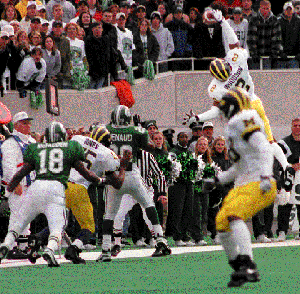
\includegraphics[height=4in]{images/woodson.png}
\caption{Woodson is a Super Human}
\label{fig:woodson}
\rule{4in}{1pt}
\end{figure}

Figures are usually horizontly centered on the page with horizontal lines at the top and botton separting it from the main text. All figures have a figure number and a caption attached to them. All figures are referred in the List of Figures by their figure number, caption text and the page number where they appear. 

This book has been formatted to show page numbers in the bottom center of the page, chapter number and name on the top header of even pages and section number and name on the top header of odd pages. Default font size for this book is 11 points. Contact the author if you would like to get a copy of the PDF version of the book with a larger font size. The original \LaTeX\ files are available upon request as well.

If you would like to know more about \LaTeX\ then I would recommend taking a look through \citet{latexcompanion}. A great, free, online resource to start learning about \LaTeX\ is https://en.wikibooks.org/wiki/LaTeX \citep{LaTeXWik0:online}.

\section*{Is This Book Suitable For You?}

Well - you wouldn't know until you spend some time with it. However, to give you a quick flavor of what you can expect from this book, I have included a sample basic data analysis example in Appendix B. If the material in Appendix B catches your fancy, looks interesting - then you are in the right place. Dig in. 

A quick word of caution though before you get too deep: this book (and the associated courses) are very hands-on. There is no point in reading this book like a sequence of text. This book should be seen more as an illustrated text - illustrated with relevant R commands and material. You should read this book alongside an RStudio session - trying all the commands there as you read along. You will need to get comfortable with a lot of command line typing, keyboard shortcuts and figuring workarounds to inevitable problems that will arise. We will often get into situations where there will be no tested/optimized/prescribed solution and we will need to figure our way out - often with some trial and error. You should be comfortable with such ambiguity.

\chapterendsymbol


\mainmatter
\pagestyle{myruled}


\part{Getting Started}



% !Rnw root = AABase.Rnw

\chapter{Advanced Big Data Analytics}

\begin{flushright}
\texttt{In God We Trust; All Others Must Bring Data}

\emph{-- Willian Edwards Deming}
\end{flushright}

\vspace{12pt}

We live in a world awash in data. All this data can be incredibly useful - it can tell us a lot - help us be better. Consider the case of WalMart in Figure: \ref{fig:frances} \citep{WhatT45:online}. WalMart collects every bit of customer data it can find - and used this data to figure out what do people buy when a hurricane is about to hit an area. I often ask this question to my students - and you can guess the usual answers - water, canned food, board games. Good guesses - but wrong. These are anticipated needs and most people purchase these items days and weeks in advance. WalMart's analysis told them that the items people buy the most just before a hurricane hits are  pop-tarts and beer. This insight has tremendous implications for the bottomline. However, extracting clear insights like this from mountains of raw data is not easy - its quite difficult in fact. We need Advanced Data Analytics techniques to do so.  

\begin{figure}
\rule{4in}{1pt}
\centering
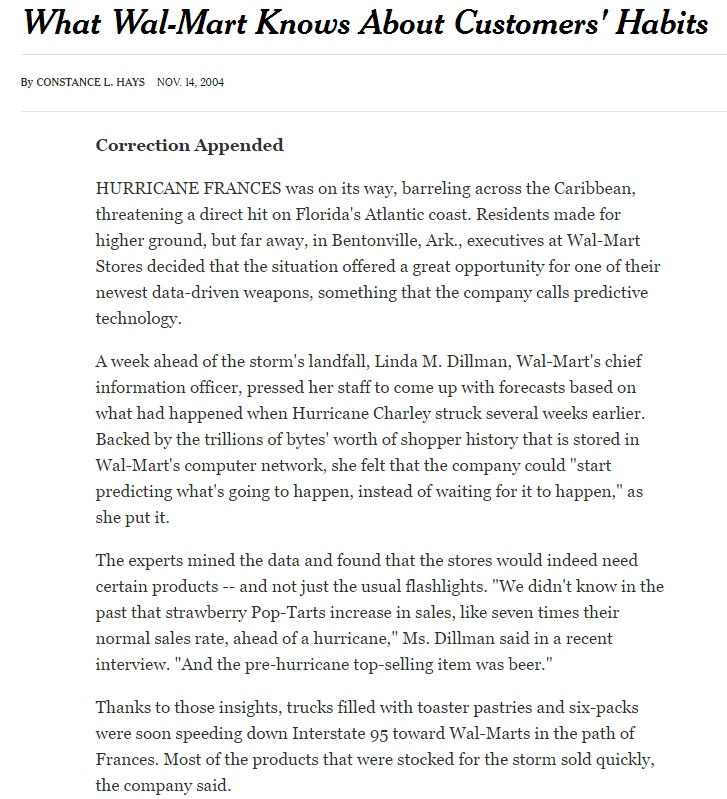
\includegraphics[height=5in]{images/NYTFrances.jpg}
\caption{WalMart Figures What to Sell in a Hurricane}
\label{fig:frances}
\rule{4in}{1pt}
\end{figure}

Success of WalMart in extracting insights from data is being replicated by different companies in different industries. NetFlix is able to predict what movies you will like. Sprint is able to predict when a customer might start considering switching services to a competitor. In a now famous incident,\mnote{The popular notion that Target knew that the girl was pregnant before even \emph{she} did; is not accurate. Sadly.} Target even managed to deduce that a teenage girl was pregnant before the girl's family knew \citep{HowTarge71:online}.  In each of these cases, companies are using specific methodologies, that we refer in this book as \rconcept{Advanced Analytics}, to transform data into insights for making better decisions.\mnote{The terms Advanced Analytics, Data Analytics and Business Analytics are often used interchangeably. We will consider them synonymous in this book.}

Our networked, connected, technology enabled world generates a lot of data that can be used for Analytics. Each time we use our credit cards, click on a web link, send a text message, even talk when your mobile phone is nearby with the Facebook app running - data is generated and stored \citep{Facebook45:online}. As you can imagine, all this data adds up. It adds up to so much that we can not hope to manage, process or analyze this much data with commonly available software in a reasonable amount of time - also known as \rconcept{Big Data}. So we need Advanced Analytics techniques that can handle Big Data.

\section{What is the Big Deal with Big Data?}

Big Data is obviously big - but size is only one aspect of Big Data that makes analyzing it difficult. Before we aanalyze Big Data, we need to first get familiar these roadblocks. They are usually referred to as the Four Vs: Volume, Velocity, Variety and Veracity \citep{Infograp69:online}.

\subsection{Volume}

The size of Big data is a constantly moving target\index{Key Concepts!Big Data!Volume} - this section will likely be obsolete by the time you get to reading it. Sure Big Data is Big - but most people do not understand just \emph{how} big it is. It is estiated that 90\% of all data that exists has been created in last two years \citep{IBMWhati26:online}. It is estimated that WalMart has collected more than 2.5  petabytes of customer data. A petabyte is $10 ^ {12}$ or one quadrillion bytes, or the equivalent of about 20 million filing cabinets' worth of text \citep{mcafee2012big}!

This incredible size of Big Data means that such data is usually stored in muliple, distributed machines. It also means that commonly available software like MS-Excel are horribly inadequate to deal with Big Data. The volume issue is actually not fully resolved in R - our tool of choice in the book. How much data we can handle in a single installation of R is usually limited by the size of RAM memory of the machine. In later chapters, we will explore various approaches to enable R to handle larger volume of data.

\subsection{Velocity}

Velocity refers to the speed with which Big Data is growing.\index{Key Concepts!Big Data!Velocity} It is the classic drinking from the firehose situation. Our data analytics tools have been fast enough to accommodate this size of incoming traffic to analyze them in real time. Our models have to be robust enough to not get quickly outdated by the new data. However, high velocity also presents a tremendous opportunity as new incoming data provides potential for continuous learning and refinement of our models.

As much of human interaction moves to social media and much of machine to machine interaction moves to Internet of Things (IoT), the velocity of Big Data will only keep growing. Again, our tool of choice - R, faces some problems in managing this deluge of data as R can comparatively slow. In later chapters, we will explore how to make R models faster to be able to handle the high velocity of Big Data.

\subsection{Variety}

Traditional statistical analysis works mainly with quantitative data; typically in the well recognized table format - columns for fields and rows for records. We do have large quantity of such data still - think WalMart transaction data or Nasdaq trading data. However, a large and growing part of today's Big Data is not in neat table format and often not even quantitative.\index{Key Concepts!Big Data!Variety} Such data may include text data (blog posts, tweets), rich media data (YouTube videos, Flickr images), sensor data (FitBit, Google Glass), location data (Google Maps, GPS data) etc. Our data analytics methodologies have to be able to make sense of all these different kinds of data.

\subsection{Veracity}

With the staggering volume, supersonic velocity and increasing variety of data come the issues of data veracity - uncertainity regarding the accuracy and trustworthiness of the data. All our data analytic models are not worth anything if they are based on suspect data. Hence, we must ensure data integrity and veracity before building data analytic models to analyze the data.

\section{Business Data Analytics}

Business analytics is the process of transforming data into insights for making better business decisions. Essentially, we want managers to no longer depend on the good old intuition, gut feel or rule of thumb. Instead we want managers to make decisions based on analyzing the available data - the so called Data Driven Decision Making.\mnote{The movie Moneyball is a good example of transitioning from an intuition/gut-feel based decision making to a data driven decision making.} Following are the three broad types of analytics that are performed as part of business data analytics. 


\subsection{Descriptive Analytics}

As the name suggests, Descriptive Analytics attempts to describe what has happened. This can take the form of descriptive statistics, data visualization or data dashboards. The focus is on explanation of an extant fact. We will cover a good part of Descriptive Analytics. Our approach will be focused on R though and will not cover specialized tools like Tableau.

\subsection{Predictive Analytics}

Predictive analytics uses models constructed from past data to predict the future or discover relationships between variables. Examples of such analytical techniques include regression, time series analytics and data mining. This is the major focus of this book - especially Regression and Data Mining.

\subsection{Prescriptive Anaytics}

Predictive analytics is concerned with finding the best course of action - including techniques such as optimization and simulation. This is NOT the main focus of this course

\section{Data Scientist}

Data Scientist is one of the fastest growing job descriptions today - the sexiest of job of 21st century according to \citet{patil2012data}.  However, being a good data scientist is a demanding job. Successful data scientists are knowledgable in statistics, programming, machine learning, data visualization and even the relevant industry domains \citep{8SkillsY88:online}.

See the Figure: \ref{fig:datascientist} for typical requirements from a data scientist position. You would note that the requirements span multiple disciplines - math and statistics, programming and databases, and communication and visualization. We will cover a good portion of these requirements in this book and associated courses. I believe that this book is a pretty good start to your journey of becoming a successful data scientist.

\begin{figure}
\rule{4in}{1pt}
\centering
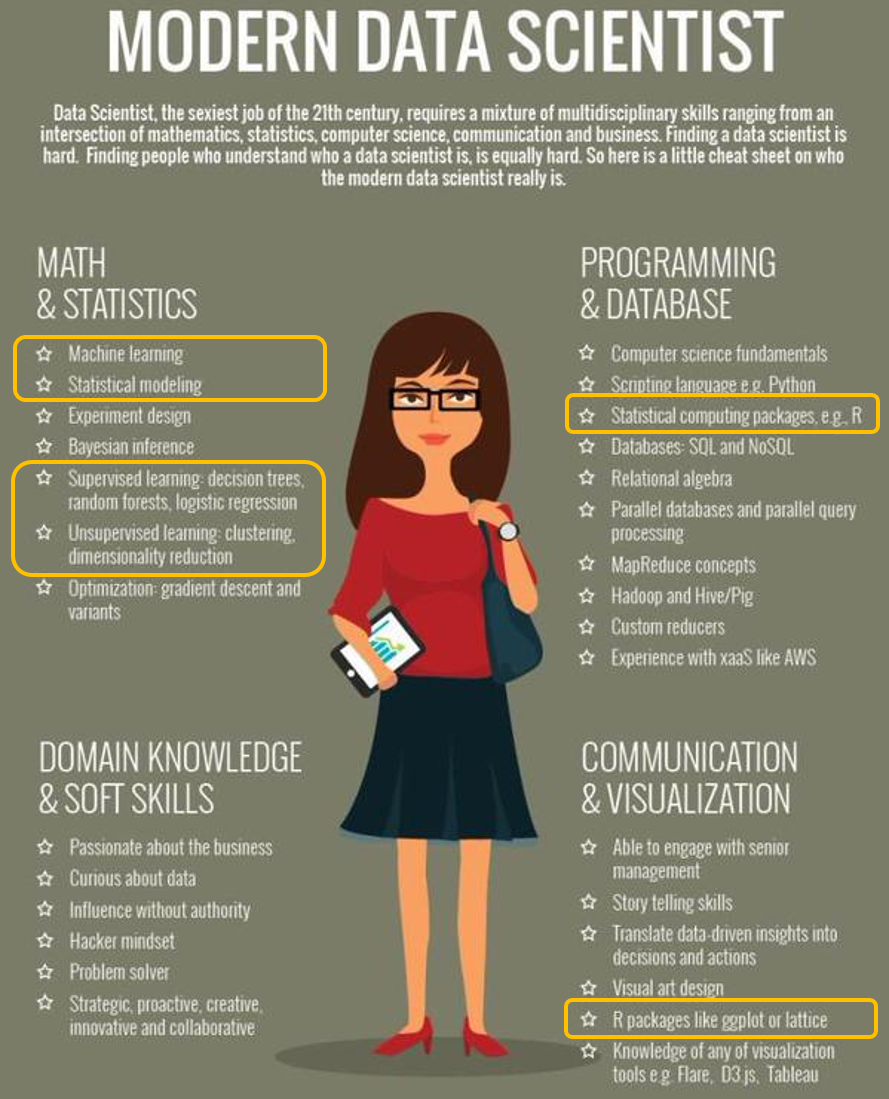
\includegraphics[height=5in]{images/datascientist.png}
\caption{Modern Data Scientist}
\label{fig:datascientist}
\rule{4in}{1pt}
\end{figure}

\chapterendsymbol




% !Rnw root = AABase.Rnw

\chapter{Our Tools: R and RStudio}

\begin{flushright}
\textbf{\texttt{In God We Trust; All Others Must Bring Data}}

\emph{-- Willian Edwards Deming}
\end{flushright}

\vspace{12pt}

R is awesome. R is also considered pretty difficult to learn. In my opinion, that's not true. In this chapter, we will quickly get out feet wet in the shallow end of the R pool - ready to jump off the deep end in the succeeding chapters.

\section{Introduction to R and RStudio}

For the purpose of this course, R is a Statistical Computing Environment. \mnote{R is a pretty awful name for anything - try googling "R" and see how relevant the search results are! It is called R after the first name of the two authors of R: Robert and Ross. The name kinda makes sense when you consider that R is based on another programming language named S.} It provides us with an underlying computer language, analysis tools and software platform for us to work with data. While R is pretty powerful, it is built by geeks for geeks. As a result, it lacks the user-friendliness needed by beginners and casual users. To help mitigate this problem, we do not directly interface with R and instead use the user friendly RStudio software as a wrapper around R. RStudio is often considered an IDE (Integrated Development Environment) for R.

\subsection{Download and Install R and RStudio} \label{sec:rinstall}

R can be downloaded from any of the mirror sites maintained by the Comprehensive R Archive Network ("CRAN"). I recommend the CRAN Mirror maintained by RStudio: \verb|https://cran.rstudio.com/|. Here you will find links to download R for Windows, Mac-OS and Linux. The current version of R available for Windows is R 3.3.1 and measures at around 70MB. Follow the directions to install the starting packages for R - often called "Base R".

Even though we will not use a bare R installtion - lets take a look at it anyway. Launch R once the installation finishes. It will look similar to Figure: \ref{fig:rbase}. This window is called the R Console. As you would note - it looks a little scary - no icons, nothing clickable, no menu even. While it is possible for us to do everything we wish to do with R just with the R Console, it really would be nice to make our experience with R a little more user friendly. Lucky for us, we have RStudio to pick up the slack here.

\begin{figure}
\rule{4in}{1pt}
\centering
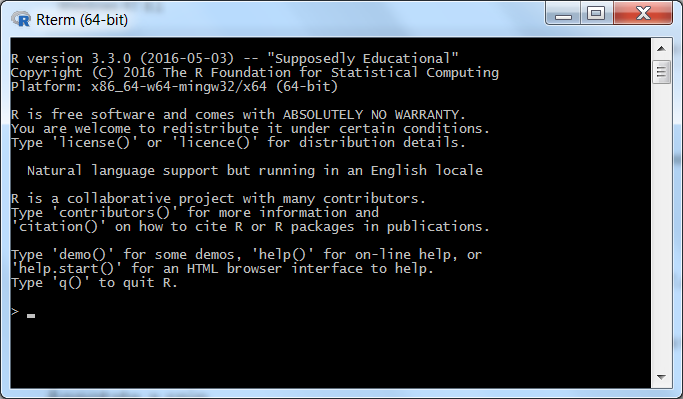
\includegraphics[height=2in]{images/rbase.png}
\caption{Staring Window of Base R Installation}
\label{fig:rbase}
\rule{4in}{1pt}
\end{figure}

Once you have finished installing R, you can download and install RStudio from: \\ 
\verb|https://www.rstudio.com/products/rstudio/download/|. There again are installers available for Windows, Mac-OS and Linux. After you are done installing RStudio, you should launch RStudio to check that everything is installed and connected properly. When you launch RStudio for the first time, you will see something similar to the Figure: \ref{fig:rstudio}.

\begin{figure}
\rule{4in}{1pt}
\centering
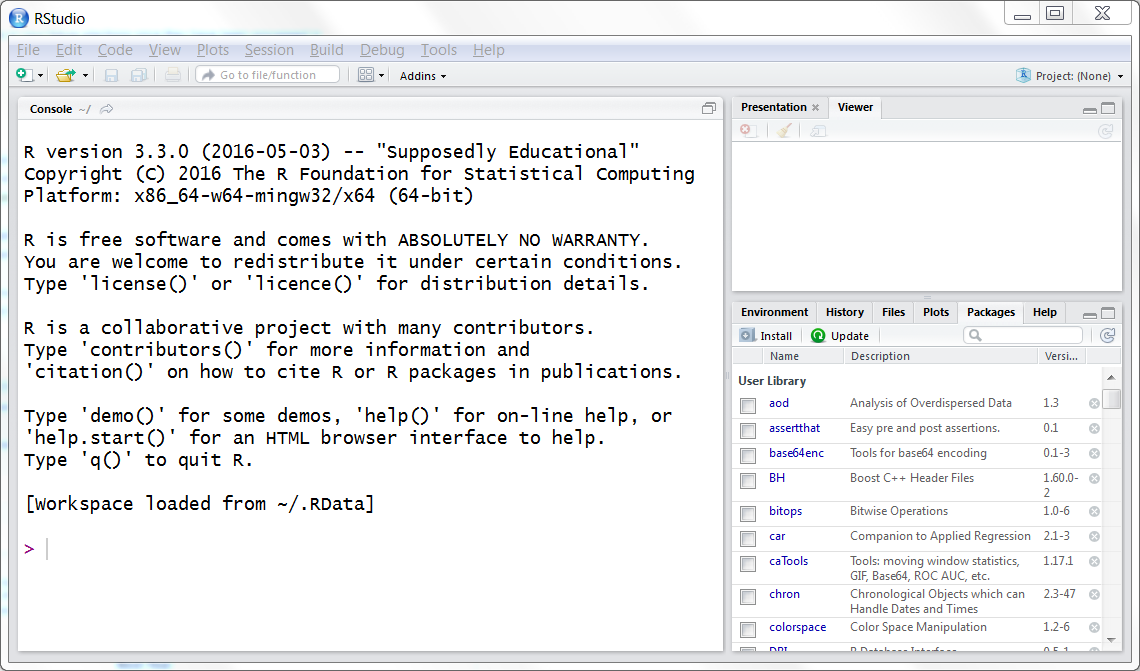
\includegraphics[height=2in]{images/rstudio.png}
\caption{Staring Window of RStudio}
\label{fig:rstudio}
\rule{4in}{1pt}
\end{figure}

The larger part of the RStudio window is same as the R Console and this is in-fact R running inside RStudio. When we launched R independently, this is the prompt that you we got. RStudio combines this direct access to R with other useful elements. In the bottom right, you have access to the file system, you can manage R packages (more about them later), read Help documentation and see various plots and charts that you will soon be building. In the top right, RStudio provides you with details of current R environment and a history of your recent R commands. If you are using Git repository for your files then you will see Git tab here.

Now that we have both R and RStudio set up, it is time for us to get started in making some use of it. Note that the R environment is used primarily by typing commands on the Console prompt. While RStudio provides GUI elements for many common tasks, we will emphasize corresponding command line versions which usually provide better control and flexibility compared to their GUI counterparts. 

\section{Useful Features of RStudio}

\subsection{Console}

The console is where you can interact directly with the R system. You can write one line at a time and immediately execute it there by pressing enter. If you wish to write more than one command in one line then you can separate the commands using the semi-colon character. The console is essentially an R session running inside RStudio. The console shows a command prompt (usually the \texttt{>}) character to indicate that you can type there. You can change the prompt by changing the options setting.\mnote{I once thought it was very clever to have this as my prompt "Sanjeev Says: ". I no longer think so.}

\begin{knitrout}
\definecolor{shadecolor}{rgb}{0.969, 0.969, 0.969}\color{fgcolor}\begin{kframe}
\begin{alltt}
\hlkwd{options}\hlstd{(}\hlkwc{prompt} \hlstd{=} \hlstr{"R> "}\hlstd{)}
\end{alltt}
\end{kframe}
\end{knitrout}

\subsection{Editor}

The editor is where you can work on and edit all of your files. This is a pure text editor - so no formatting of any kind. You will mostly be working with RMD files here. The tab panel at the top of the editor allows you to work on multiple files at once. The editor window is hidden when you start RStudio as you usually don't have a file to edit when you begin. Once you create/open a new file then they will open in the editor window and you can edit them. The editor window helpfully shows you the line numbers in left column and the cursor positioning in the line at the bottom left corner. The bottom right corner shows you the file type that you are working on. There are usual icons for saving a file, finding, spell check etc on the top bar. See Figure: \ref{fig:editor} for an example.

\begin{figure}
\rule{4in}{1pt}
\centering
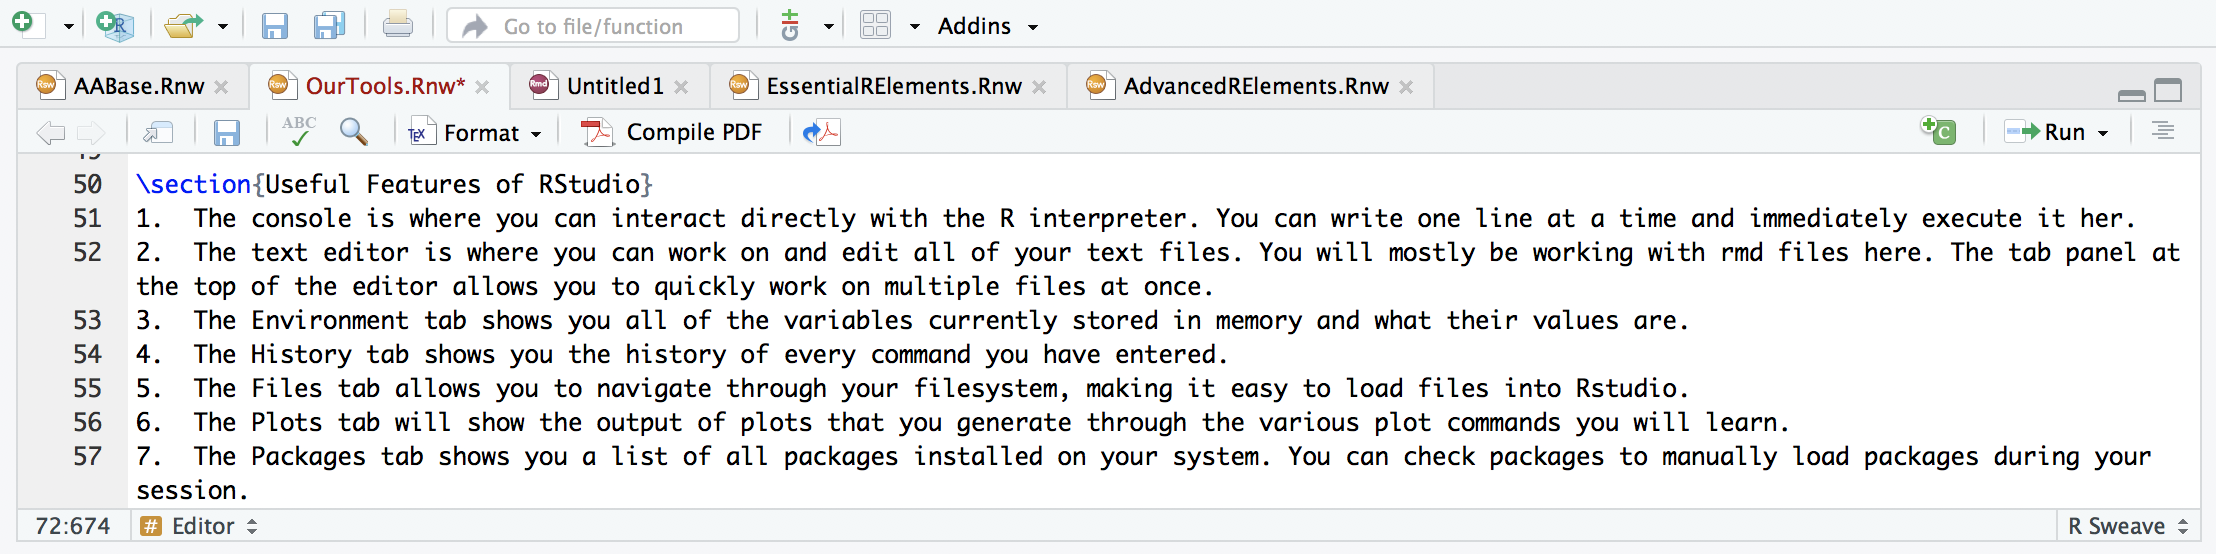
\includegraphics[width=5in]{images/editor.png}
\caption{Editor Window}
\label{fig:editor}
\rule{4in}{1pt}
\end{figure}

\subsection{Environment}

The Environment tab shows you all of the variables currently stored in memory and what their values are.\mnote{We haven't said what variables are as yet. Hold on - its coming in the next chapter.} The tab in fact shows all the objects that currently exist in your R session.\mnote{Objects will be discussed very soon, later in this chapter} Environment tab is a very useful place to have a quick look at the state of your current R session. The environment tab has a handy broom icon for deleting all the objects that exist and clearning your environment. You can, of course, do that using a command as well - \rcommand{rm} for remove or delete. The command \rcommand{ls} generates a list of all the objects in the environment.

\begin{knitrout}
\definecolor{shadecolor}{rgb}{0.969, 0.969, 0.969}\color{fgcolor}\begin{kframe}
\begin{alltt}
\hlkwd{rm}\hlstd{(}\hlkwc{list} \hlstd{=} \hlkwd{ls}\hlstd{())}  \hlcom{#Delete every object in the environment}
\end{alltt}
\end{kframe}
\end{knitrout}

\subsection{History}

The History tab shows you the history of all the commands you have entered in the Console window. You can use available icons on top to search through the history or delete items from the history. Two very useful icons are for transferring commands to the console and to the source. See details in Figure: \ref{fig:history}. The \texttt{To Console} allows you to select one or more commands from the history and transfers them to the Console window where you can run them by pressing Enter. The \texttt{To Source} sends the selected commands to the Editor window, to the currently open and active file.

\begin{figure}
\rule{4in}{1pt}
\centering
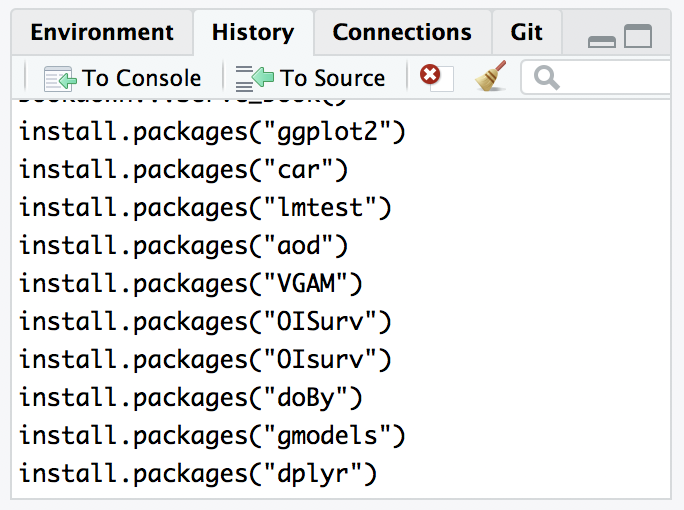
\includegraphics[height=1.5in]{images/history.png}
\caption{History Window}
\label{fig:history}
\rule{4in}{1pt}
\end{figure}

\subsection{Files}

The Files tab allows you to navigate through your filesystem, making it easy to load files into Rstudio. It shows the content of the current working directory when RStudio starts. You can navigate through the file system of your machine using the available options. The top icons provide ability to create a new folder, delete selected files, rename selected files and refresh file listings. The \texttt{More} option reveals further functionalities including two useful ones: the ability to set the currently displayed directory as the working directory and the ability to get the Files tab to display the contents of the current working directory. Figure: \ref{fig:files} shows the options.

\begin{figure}
\rule{4in}{1pt}
\centering
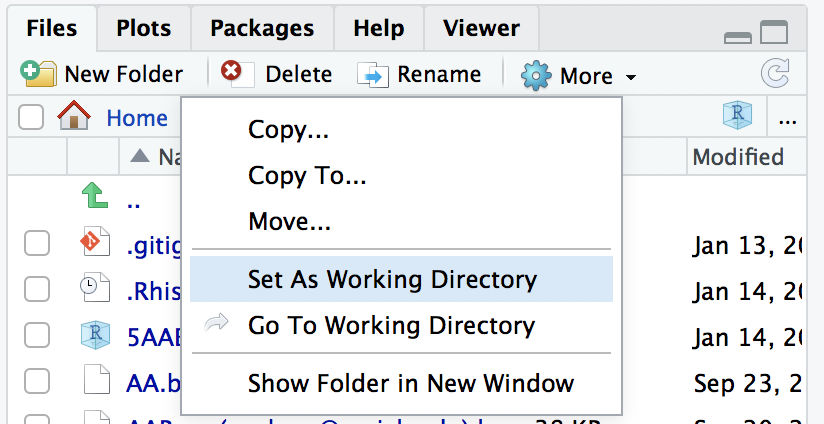
\includegraphics[height=1.5in]{images/files.png}
\caption{Files Window}
\label{fig:files}
\rule{4in}{1pt}
\end{figure}

\subsection{Plots}

the Plots tab shows the plots generated by the commands typed in the Console. Figure: \ref{fig:plots} show the plot generated by the command \texttt{plot(cars)} command in the Plots tab. As you can see, you can use options to zoom in/out and export the plot image as an image file or a PDF document.\mnote{Plots made by R are Vector graphics and hence should be saved in vector formats like PNG and not bitmap formats like JPG}

\begin{figure}
\rule{4in}{1pt}
\centering
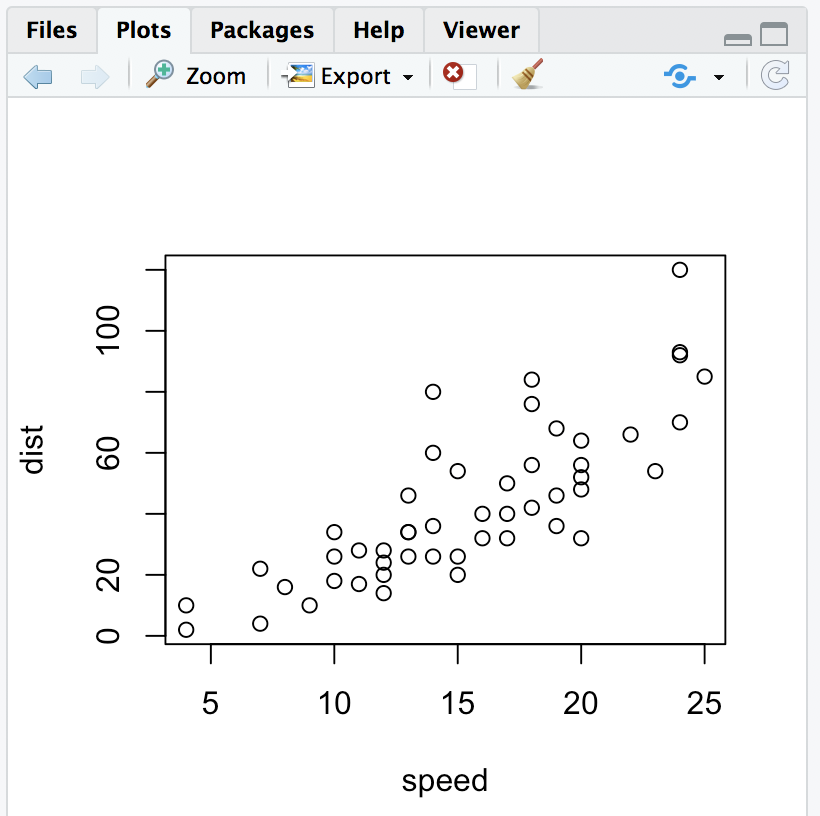
\includegraphics[height=2in]{images/plots.png}
\caption{Plots Window with a Demo Plot}
\label{fig:plots}
\rule{4in}{1pt}
\end{figure}

\subsection{Packages}

The Packages tab shows you a list of all the packages installed on your system and their version number. You can check the checkbox next to the package name to manually load packages during your R session. You will also find icons for installing and updating packages. A search icon allows for searching among installed packages. 

\subsection{Help}

As the name suggests, the Help tab can be used to find Help documentation on specific keywords. You can search for a keyword in the search field for looking at corresponding help documentation. If you write a help command in the console, then the output of that will also show in the Help tab. For example, if you type the command below (looking for help on "help"), you will get the help documentation as shown in Figure: \ref{fig:help}.

\begin{knitrout}
\definecolor{shadecolor}{rgb}{0.969, 0.969, 0.969}\color{fgcolor}\begin{kframe}
\begin{alltt}
\hlkwd{help}\hlstd{(}\hlstr{"help"}\hlstd{)}
\end{alltt}
\end{kframe}
\end{knitrout}

\begin{figure}
\rule{4in}{1pt}
\centering
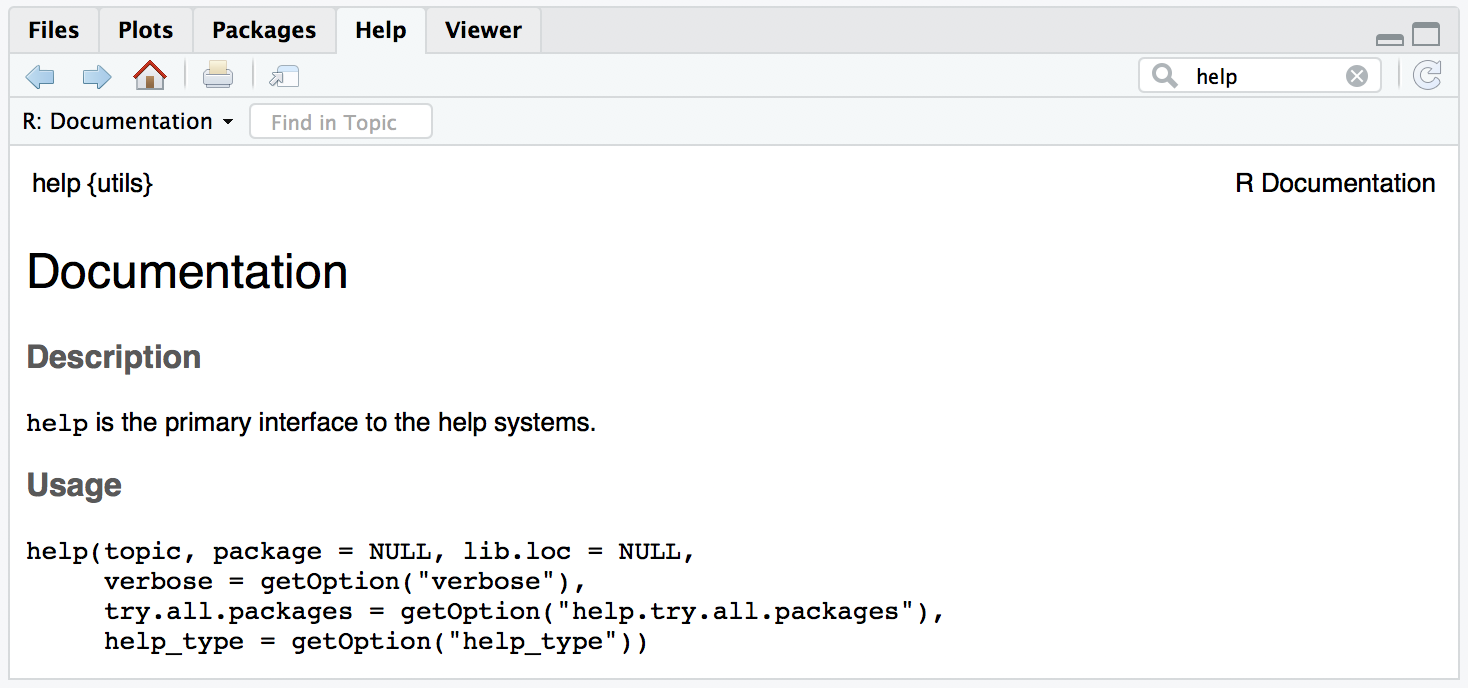
\includegraphics[height=2in]{images/help.png}
\caption{Help Windown when looking for help on "help"}
\label{fig:help}
\rule{4in}{1pt}
\end{figure}

\section{Helpful Menu Items and Keyboard Shortcuts}

\section{Essential R Tips \& Tricks}

\subsection{R is Case Specific and Space Neutral}

Everything in R is case specific. In R, upper case letters are considered completely different than their lower case counterparts. R will show no mercy if you mistype something in a difference case. However, R is pretty flexible about spaces and will usually accept multiple (or none) spaces where the default expectation is one space. 

\subsection{Comments and Line Continuation}

You can add your comments/remarks in your R code by inserting the \verb|#| character. Any text after the \verb|#| character will be ignored by R during execution. It is essential that sufficient comments are added to your R code so that the code remains understandable and if you share your code with somebody else then they have a way of figuring out what you are trying to do, why and how.

R is smart enough to figure when the command is not finished and allows you to continue typing on the next line. This usually works well when there are un-finished parentheses or operators at the end. R indicates that it is expecting further inputs by showing the character \texttt{+} at the beginning of the next line. See Figure: \ref{fig:incomplete} for an example.

\begin{figure}
\rule{4in}{1pt}
\centering
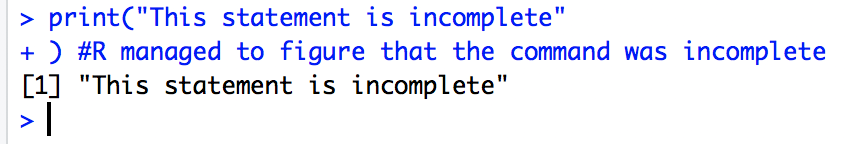
\includegraphics[height=0.5in]{images/incomplete.png}
\caption{Line Continuation for Incomplete Commands}
\label{fig:incomplete}
\rule{4in}{1pt}
\end{figure}

\subsection{Naming Conventions}

Object names in R can consist of any combination of alphanumeric characters (\texttt{a-z}, \texttt{A-Z}, \texttt{0-9}) as well as underscore \texttt{-} and period \texttt{.} characters. Object names should not include special characters such as \texttt{?} or space. Object names must start with a letter or a period. Special care should be taken to not include one of the reserved keywords (like $function$ or $help$) as object names.


\section{RMarkdown (RMD) Files}

We will use extensive ise of RMarkdown files in the class. Markdown is a simple formatting syntax for authoring documents. RMarkdown allows you to create Markdown documents with embedded R code in them. RMarkdown documents can then be rendered in variety of output formats such as HTML, PDF, and MS Word documents. 

RStudio streamlines the process of creating an RMarkdown file. Getting started is easy - in RStudio, go File -> New File -> R Markdown (or Alt-F-F-M). This will start a new RMD file for you. It needs some startup information to proceed first, as shown in the image below:

%![Figure: RMD Startup Dialog](RMDStart.png)

Title and Author are self explanatory. As the dialog suggests, you can choose HTML, PDF of Word as default output formats. PDF and Word require you to have a local installed version of TeX or MS-Word. For our class, I recommend that you use HTML as the default output - it is device and platform independent - and capable of handling variety of rich media. We will see later how to include dynamic content like animation and user interaction in these HTML files as well.

Once you say OK, you will be taken to the default start page. This page has some content already to help you started. You should be able to see the preamble right on top that will generate your document headers and also control various options:

\begin{verbatim}
```
title: "Untitled"
author: "Dr. Sanjeev Kumar"
date: "May 5, 2018"
output: html_document
```
\end{verbatim}

You can make changes by either hand-editng the information above or by clicking the Edit Option icon (which looks like a gear) and choosign your options. For example, the preamble for one of my document looks like the following:

\begin{verbatim}
```
title: "How To Write RMarkdown Files"
author: "Dr. Sanjeev Kumar"
date: "May 5, 2016"
output:
  html_document: 
    highlight: tango
    number_sections: yes
```
\end{verbatim}

Now you can go ahead and add content to your document. When you want to create the output,  click the \emph{Knit} button and a document will be generated that includes both content as well as the output of any embedded R code chunks within the document. We will see later in the document how to embed R code in RMD files.

It is easy to format RMarkdown files and embed R code in them. For more details on using R Markdown see http://rmarkdown.rstudio.com.

\section{Embedding R Code Blocks in RMD Files}

\subsection{Embedding Options}

\begin{description}
  \item[echo]
  \item[eval]
  \item[cache]
  \item[label]
  \item[fig.height/width]
\end{description}

\subsection{Embedding Code Blocks of Other Languages }


\subsection{Embedding in-line R Code}


\subsection{Reproducibility of Data Analysis}

A key advantage of using an RMD file is that the output contains both the R code and the output. That allows for a precise matching of what steps were performed to reach a specific output. Consider the example of a complex chart made in MS-Excel - you would be hard pressed to figure out what exactly was done to create that chart. Whether the chart has some data manipulation in it, whether the chart inadvertently includes a mistake - there is no transparency - and hence you are likely to not have much trust in the chart. In the case of RMD files on the other hand, the entire process of creating the chart is right there in the form of R commands. Anybody else with the same data and the same commands will reach exactly the same output. Your analysis can be reproduced by anybody else - imporving the reliability and trustworthiness of your analysis.

We discussed "veracity" as one of the four Vs of Big Data. Doing data analytics in a way that is reproducible (e.g through an RMD file) goes a long way towards establishing confidence in the results of the analysis.

\section{Key Features of R/RStudio Ecosystem}

\subsection{Open Source Software}

Open Source Software is a broad term for software that is developed by a community of volunteers and is available free of charge for you and I to use. R is open source with a strong and dedicated community that takes the stewardship of R very very seriously. 
As R is open source, the underlying computer code (the source code) is available for anyone to view and modify. All these extra eyes looking at the code usually means a more reliable, error free and malware resistant software. 

Open source nature of R has both positive and negative impacts. On the positive side, the community helps extend R rapidly by building new packages with new capabilities very quickly. On the negative side, the R platform is built by experts for experts - the focus is on capability and precision - not on ease of use. This makes R a swiss army knife of that is capable of doing almost everything possible in data domain but a knife that can be difficult to learn how to use.

\subsection{Extensability of R}

R is desiged to be easily extended. You, me and everyone else can write new functionalities for R and have it available for everyone in the world to download and use. The R community has been writing extensions for decades now and the result is a library of thousands of packages. If there is anything data analysis related that you want to do, chances are that somebody else wanted to do it too, has already built a package for it that you can download and use. 

Easy extensability of R is one of the main reasons why R remained the most capable, cutting edge data analytical platform for decades now. R community has written packages to allow you write SQL commands, C++ commands, build geo-maps, build predictive models - all within the R platform. New developments tend to get incorporated in R much faster than in competing statistical software such as Stata, SAS or SPSS.     

\subsection{Usability of R}

R is not graphical. Much of R's capabilities are accessed through typing R commands rather than clicking buttons or accessing menus. R commands allow a level of precision and flexibility that is typically now achievable through a graphical interface. Doing complex tasks successfully in R involves writing a sequence of R commands that are closer to coding in a programming language than using a point and click software.

While R can be considered to have a steep learning curve, it should be noted that once you get through the learning curve and get used to R's syntax, you can slice through complex data analysis with much greater speed and capability than competing alternatives. In my opinion, the learning curves for R and competing graphical alternatives look like Figure: \ref{fig:lcurve}. R starts slower and has a difficult jumpstart but if you stay with it for a little bit then R handily outperforms the graphical alternatives.

\begin{figure}
\centering
\rule{4in}{1pt}
\begin{knitrout}
\definecolor{shadecolor}{rgb}{0.969, 0.969, 0.969}\color{fgcolor}
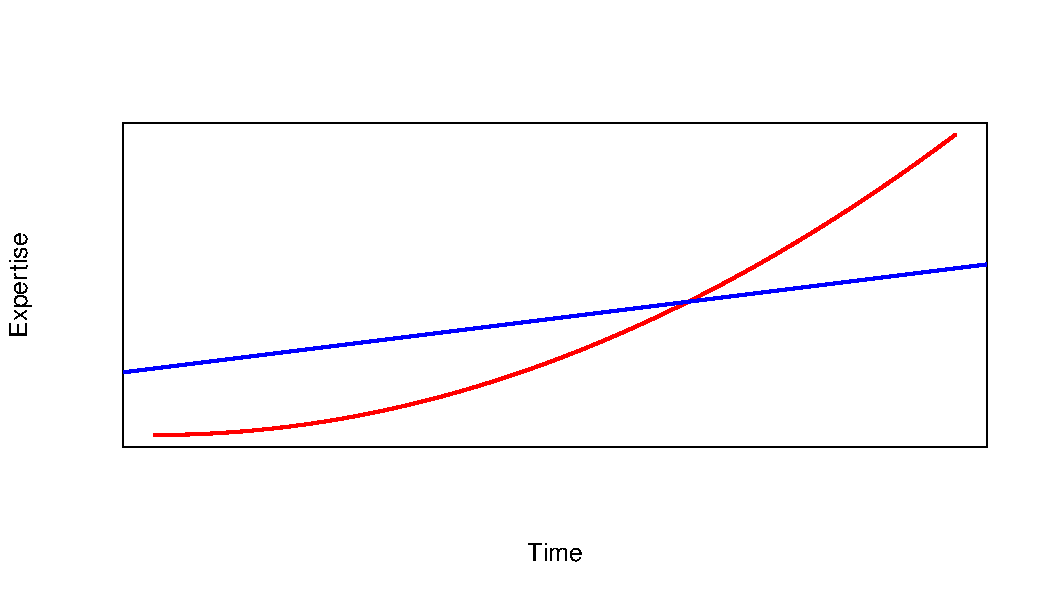
\includegraphics[width=\maxwidth]{figure/unnamed-chunk-8-1} 

\end{knitrout}
\caption{Learning Curves for R (red) and alternatives (blue)}
\label{fig:lcurve}
\rule{4in}{1pt}
\end{figure}

BTW - the plot in Figure: \ref{fig:lcurve} was generated using R. Here is the code for it:
\begin{knitrout}
\definecolor{shadecolor}{rgb}{0.969, 0.969, 0.969}\color{fgcolor}\begin{kframe}
\begin{alltt}
\hlcom{# Code to generate the Learning Curve Plot}
\hlkwd{curve}\hlstd{(x}\hlopt{^}\hlnum{2}\hlstd{,} \hlkwc{from} \hlstd{=} \hlnum{0}\hlstd{,} \hlkwc{to} \hlstd{=} \hlnum{3}\hlstd{,} \hlkwc{xlab} \hlstd{=} \hlstr{"Time"}\hlstd{,} \hlkwc{ylab} \hlstd{=} \hlstr{"Expertise"}\hlstd{,} \hlkwc{col} \hlstd{=} \hlstr{"red"}\hlstd{,}
    \hlkwc{lwd} \hlstd{=} \hlnum{2}\hlstd{,} \hlkwc{xaxt} \hlstd{=} \hlstr{"n"}\hlstd{,} \hlkwc{yaxt} \hlstd{=} \hlstr{"n"}\hlstd{)}
\hlkwd{abline}\hlstd{(}\hlkwc{a} \hlstd{=} \hlnum{2}\hlstd{,} \hlkwc{b} \hlstd{=} \hlnum{1}\hlstd{,} \hlkwc{col} \hlstd{=} \hlstr{"blue"}\hlstd{,} \hlkwc{lwd} \hlstd{=} \hlnum{2}\hlstd{)}
\end{alltt}
\end{kframe}
\end{knitrout}

\subsection{R is NOT Verbose}

In fact R is very very concise. It will not give you an output until you ask for it. This is very different than most statistical software that tend to overwhelm the user with every possible output possible. R allows you the flexibility to specifically request the levek of detail you need. By default, R will provide only the minimal amount of output.

\subsection{Object Oriented Programming}

\subsection{R Community's Sense of Humor}

R community is a hard working one - they are continuously building new and latest packages - making the R ecosystem even better. R community is also a fun one - a clever one at the very least. For example - look at the nickname for the current version:
\begin{knitrout}
\definecolor{shadecolor}{rgb}{0.969, 0.969, 0.969}\color{fgcolor}\begin{kframe}
\begin{alltt}
\hlstd{version}\hlopt{$}\hlstd{nickname}
\end{alltt}
\begin{verbatim}
## [1] "Kite-Eating Tree"
\end{verbatim}
\end{kframe}
\end{knitrout}

The R community is very helpful and will answer your questions if you post on relevant forums like StackExchange.com. However, they don't suffer fools and xpect people who ask questions to have done their homework. Over the years, the R community has developed an extensive knowledgebase that is only a google search away for you. As you go further in your exploration of R, attempt to learn from the community and hopefully one day be a bonafide member of the community.

\section{Common Issues, Pitfalls, Bugs, Obstacles and Their Solutions}

This section is my master list of common issues that students encounter when they start working with R. You may want to not read this in full right now - treat this as a reference section. When you run into an issue, come by here and see if I have a solution for you.

\subsubsection*{I have an older R installtion. How do I upgrade it?}

You might have an old, not updated version of R in your machine. You can check the current version of your R by running the \rcommand{version} command. If you have an older version and if you are in a Windows machine, then upgrading your R installation is easy with the \rpackage{installr} package. The \texttt{installr} package has the handy \rcommand{updateR} command that will automatically update your R installation to the latest one. A sample code to accomplish this is below:

\begin{knitrout}
\definecolor{shadecolor}{rgb}{0.969, 0.969, 0.969}\color{fgcolor}\begin{kframe}
\begin{alltt}
\hlcom{# Sample code, not being evaluated here}
\hlkwd{install.packages}\hlstd{(}\hlstr{"installr"}\hlstd{)}  \hlcom{# install the installr package }
\hlkwd{library}\hlstd{(installr)}
\hlkwd{updateR}\hlstd{()}  \hlcom{# updating your R version}
\hlstd{version}  \hlcom{# command for checking your current R version}
\end{alltt}
\end{kframe}
\end{knitrout}

If you happen to be in a Mac or Linux machine, then you would want to download the current version of R and install. This process is similar to installing a fresh new installation of R as discussion in Section: \ref{sec:rinstall}.

\subsubsection*{Help - I am not being able to install any packages!}

If you are unable to install R packages, there are a few things we can try.\mnote{I am not going to insult your intelligence by asking you to make sure that you have a live Internet connection!} First thing to check would be your anti-virus software. Several anti-virus software balk at allowing R to perform tasks that may be interpreted as a security risk (for example - downloading anf installing packages from the Internet). You can try to work around this by disabling/uninstalling your anti-virus or adding R to the exceptions list in the anti-virus.

You may also want to check whether you have administrator access in the machine you are working on. Several essential tasks in R require the user to have administrator access.

Lastly, R may be attempting to install packages into a directory that it does not have write permissions on. This can sometimes happen if you are on a computer on a network with mapped drives. You can work around this problem by asking R to install your packages in a safe, editable directory where you have write access. R installs all packages in a library directory - you can find out the current location of the library directory with the \rcommand{.libPaths} command. You can use the \texttt{.libPaths} command to then add a directory location as your personal library location so that R can then install packages in that directory. A sample code to accomplish this is shown below:

\mnote{Last command commented as C:/Whatever does not exist obviously - so would have resulted in an error.}
\begin{knitrout}
\definecolor{shadecolor}{rgb}{0.969, 0.969, 0.969}\color{fgcolor}\begin{kframe}
\begin{alltt}
\hlkwd{.libPaths}\hlstd{()}  \hlcom{#Shows the current library path}
\end{alltt}
\begin{verbatim}
## [1] "/Library/Frameworks/R.framework/Versions/3.4/Resources/library"
\end{verbatim}
\begin{alltt}
\hlcom{# I have two folders in my library path currently You can add your own}
\hlcom{# library folder to the path libPaths( c( .libPaths(),}
\hlcom{# 'C:/Whatever/Whatever...') )}
\end{alltt}
\end{kframe}
\end{knitrout}

\subsubsection*{Why is the edit command not working for me?}

One of the first R commands that gives trouble is the \rcommand{edit} command. As the name suggests, \texttt{edit} is used for editing data - typically it shows the data to be edited in a table format with editable cells. This specific command (and its cousin, the \rcommand{fix} command) seems to be very sensitive to the keyboard layouts, especially on Apple machines. This problem is hardware oriented and may prove difficult to solve. I usually recommend to ignore these two commands and take care of your data editing needs using alternative methods. If you were using \texttt{edit} for only viewing the data, then \rcommand{View} is a good alternative for that.


\chapterendsymbol




% !Rnw root = AABase.Rnw

\chapter{Essential R Language Elements}

\begin{flushright}
\textbf{\texttt{In God We Trust; All Others Must Bring Data}}

\emph{-- Willian Edwards Deming}
\end{flushright}

\vspace{12pt}

In this chapter we will start playing with some basic R functionalities and start getting comfortable with typing commands in the R console. All code examples you see in the chapter are opportunities for you to type them in R Console yourself and see whether you get the same output. There is no better way to find your way around R than to get your hands dirty - and no better time than now. So lets get started.

\section{Arithmatic Operators}

You can use R as a glorified calculator. All arithmatic calculations can be easily performed using \rconcept{Arithmatic Operators} like + (addition), - (subtraction), * (multiplication), / (division) and \verb|^| (exponent).
\begin{knitrout}
\definecolor{shadecolor}{rgb}{0.969, 0.969, 0.969}\color{fgcolor}\begin{kframe}
\begin{alltt}
\hlnum{10} \hlopt{+} \hlnum{20}  \hlcom{#As you can see - spaces don't matter, mostly.}
\end{alltt}
\begin{verbatim}
## [1] 30
\end{verbatim}
\begin{alltt}
\hlnum{20}\hlopt{/}\hlnum{5}
\end{alltt}
\begin{verbatim}
## [1] 4
\end{verbatim}
\begin{alltt}
\hlnum{16}\hlopt{^}\hlnum{0.5}  \hlcom{# Usual Arithmatic Operators: +, -, * , /, ^}
\end{alltt}
\begin{verbatim}
## [1] 4
\end{verbatim}
\end{kframe}
\end{knitrout}

You would note that the outputs to the commands have this \verb|[1]| before them. The number indicates how many values there are in the output. Since the commands above lead to a single output value - you see the \verb|[1]| there.

When you have complicated Arithmatic Expressions, R follows usual \rconcept{Arithmatic Operator Precedance}: Brackets, Exponent, Division and Multiplication, Addition and Subtraction - in that order. Go Left to Right for the same precedance. Of course it is preferable to put in enough paratheses so that you are not relying on R's operator precedance for accurate execution of your commands. 
\begin{knitrout}
\definecolor{shadecolor}{rgb}{0.969, 0.969, 0.969}\color{fgcolor}\begin{kframe}
\begin{alltt}
\hlnum{5} \hlopt{+} \hlnum{8}\hlopt{/}\hlnum{2} \hlopt{*} \hlnum{4} \hlopt{-} \hlnum{3}  \hlcom{# First * then / then + then - }
\end{alltt}
\begin{verbatim}
## [1] 18
\end{verbatim}
\begin{alltt}
\hlcom{# You should include enough parantheses}
\hlstd{(}\hlnum{5} \hlopt{+} \hlnum{8}\hlstd{)}\hlopt{/}\hlstd{((}\hlnum{2} \hlopt{*} \hlnum{4}\hlstd{)} \hlopt{-} \hlnum{3}\hlstd{)}
\end{alltt}
\begin{verbatim}
## [1] 2.6
\end{verbatim}
\end{kframe}
\end{knitrout}

Two arithmatic operators that many are not familiar with are: \rconcept{Integer Division} and \rconcept{Remainder} operators. The \texttt{Integer Division} operator: \verb|%/%|, provides just the quotient for a division operation while the \texttt{remainder operator}: \verb|%%|, provides just the remainder for a division operation.

\begin{knitrout}
\definecolor{shadecolor}{rgb}{0.969, 0.969, 0.969}\color{fgcolor}\begin{kframe}
\begin{alltt}
\hlnum{10}\hlopt\hlnum{3}  \hlcom{# Integer division - only gives the quotient as the output}
\end{alltt}
\begin{verbatim}
## [1] 3
\end{verbatim}
\begin{alltt}
\hlnum{10}\hlopt\hlnum{3}  \hlcom{# The counterpart to %/%, gives remainder as the output}
\end{alltt}
\begin{verbatim}
## [1] 1
\end{verbatim}
\end{kframe}
\end{knitrout}

\section{Logical Operators}

Just as arithmatic expressions evaluate to a numerical result, logical expressions evaluate to a logical result - either \texttt{TRUE} or \texttt{FALSE}. \mnote{Note the upper case format for the two keywords. The letters T and F are also acceptable values as shorthand for TRUE and FALSE} Logical expressions can be created using \rconcept{Logical Operators}: equal to (==), greate than (>), less than (<), greater than or equal to (>=), less than or equal to (<=) and finally, not equal to (!=).

\begin{knitrout}
\definecolor{shadecolor}{rgb}{0.969, 0.969, 0.969}\color{fgcolor}\begin{kframe}
\begin{alltt}
\hlnum{10} \hlopt{>} \hlnum{20}  \hlcom{#Should evaluate to FALSE}
\end{alltt}
\begin{verbatim}
## [1] FALSE
\end{verbatim}
\begin{alltt}
\hlnum{12.37} \hlopt{<=} \hlnum{23.66}  \hlcom{#Should evaluate to TRUE}
\end{alltt}
\begin{verbatim}
## [1] TRUE
\end{verbatim}
\begin{alltt}
\hlstd{(}\hlnum{10}\hlopt{/}\hlnum{3}\hlstd{)} \hlopt{==} \hlstd{(}\hlnum{30}\hlopt{/}\hlnum{9}\hlstd{)}  \hlcom{#Should evaluate to TRUE}
\end{alltt}
\begin{verbatim}
## [1] TRUE
\end{verbatim}
\end{kframe}
\end{knitrout}

Logical values can be combined using \rconcept{AND} and \rconcept{OR} constructs. When combining two logical values using \texttt{OR}, the resulting value is \texttt{TRUE} if any of the two values are \texttt{TRUE}. When combining two logical values using \texttt{AND}, the resulting value is \texttt{TRUE} only of both the values are \texttt{TRUE}. The command for \texttt{AND} is \rcommand{\&} while the command for \texttt{OR} is the \texttt{|} character.

\begin{knitrout}
\definecolor{shadecolor}{rgb}{0.969, 0.969, 0.969}\color{fgcolor}\begin{kframe}
\begin{alltt}
\hlstd{(}\hlnum{10} \hlopt{>} \hlnum{20}\hlstd{)} \hlopt{|} \hlstd{(}\hlnum{12.37} \hlopt{<=} \hlnum{23.66}\hlstd{)}  \hlcom{#Should evaluate to TRUE}
\end{alltt}
\begin{verbatim}
## [1] TRUE
\end{verbatim}
\begin{alltt}
\hlstd{(}\hlnum{10} \hlopt{>} \hlnum{20}\hlstd{)} \hlopt{&} \hlstd{(}\hlnum{12.37} \hlopt{<=} \hlnum{23.66}\hlstd{)}  \hlcom{#Should evaluate to FALSE}
\end{alltt}
\begin{verbatim}
## [1] FALSE
\end{verbatim}
\end{kframe}
\end{knitrout}

You can use \rconcept{NOT} operator to convert a \texttt{TRUE} value to \texttt{FALSE} and vice versa - the corresponding command is \texttt{!} character. You can use logical operators to compare non-numeric values as well.

\begin{knitrout}
\definecolor{shadecolor}{rgb}{0.969, 0.969, 0.969}\color{fgcolor}\begin{kframe}
\begin{alltt}
\hlopt{!}\hlnum{TRUE}  \hlcom{#Should evaluate to FALSE}
\end{alltt}
\begin{verbatim}
## [1] FALSE
\end{verbatim}
\begin{alltt}
\hlstr{"Dog"} \hlopt{>} \hlstr{"Cat"}  \hlcom{#As everybody know, this is TRUE}
\end{alltt}
\begin{verbatim}
## [1] TRUE
\end{verbatim}
\end{kframe}
\end{knitrout}

As the example above shows, comparing non-numeric values \mnote{We have not discussed different data types yet. Values enclosed in quote marks are text values, typically called Strings} can result in interesting results. When two strings are compared, they are essentially compared one character at a time. In the example above, the character C is compared with character D. The comparison is based on the Unicode number associated with the characters. As D has a higher Unicode number than C, "Dog" is considered higher than "Cat". \mnote{Interesting thought experiment: \\ 1000 > 50: True or False? \\ "1000" > "50": True or False?}

\section{Variables}

R keeps all data in \rconcept{Variables}. Variables can be thought of as a space in computer's memory where R can store data. Once we have created a variable, we can then use the variable name to access, manipulate and work with the data kept in the variable. Variables are created using the \rconcept{Assignment Operator} written as \rcommand{<-}. The arrow indicates the direction of assignment. Operators also exist to do assignment in the opposite direction (\texttt{->}) and do the same operation as assignment operator. R also supports the assignment operator command used by many other programming languages (\texttt{=}) but it is customary to use the right-to-left version of assignment operator. \mnote{I find the R version of assignment operator to be much more intuitive as the direction of value assignment is clearly specified. The = charater usually confuses beginners into thinking that we are "equating" values instead of the correct interpretation of "assigning" value from one side to the other.}

\begin{knitrout}
\definecolor{shadecolor}{rgb}{0.969, 0.969, 0.969}\color{fgcolor}\begin{kframe}
\begin{alltt}
\hlstd{revenue} \hlkwb{<-} \hlnum{100}  \hlcom{#Typical way of creating a variable and assigning value}
\hlcom{# Above is the recommended approach}
\hlstd{revenue} \hlkwb{=} \hlnum{100}  \hlcom{#Alternate way of doing same as above}
\hlcom{# 100 -> revenue #Reverse direction assignment}
\hlstd{revenue} \hlkwb{<-} \hlstd{revenue} \hlopt{+} \hlnum{300}  \hlcom{#Performing calculations}
\hlkwd{print}\hlstd{(revenue)}  \hlcom{#Printing/showing the value inside the variable}
\end{alltt}
\begin{verbatim}
## [1] 400
\end{verbatim}
\end{kframe}
\end{knitrout}

The first three line of the code above should be read as the value 100 is assigned to the variable \emph{revenue}. In the fourth line, we add 300 to the current value of variable \emph{revenue} and the resulting value (in this case 400) is then assigned to the variable \emph{revenue}. So the value in the variable \emph{revenue} is now 400, which is shown as output in the last line.

A numeric variable like \emph{revenue} above can be used just like a number to perform all usual arithmetic operations.

\section{Variable Data Types}

Variables can store  different types of data. We saw integer numerical data in the examples above. Other common data types include floating point numbers (fractional numbers), characters data (i.e. a single character), text data (called strings - as in string of characters) and logical data (true or false). We can find the data type of a variable by using the \rcommand{class} command.

\begin{knitrout}
\definecolor{shadecolor}{rgb}{0.969, 0.969, 0.969}\color{fgcolor}\begin{kframe}
\begin{alltt}
\hlstd{numvalue} \hlkwb{<-} \hlnum{20.56}  \hlcom{#Creating a numeric variable}
\hlkwd{class}\hlstd{(numvalue)}  \hlcom{#Finding data type of numvalue variable}
\end{alltt}
\begin{verbatim}
## [1] "numeric"
\end{verbatim}
\end{kframe}
\end{knitrout}

\subsection{Numeric Data}

Variables of numeric data type can store both integers and floating point values. Unlike many programming languages, R does not have various different kinds of integers and floating point numbers defined to optimize memory usage. 

\subsection{String Data}

\rconcept{String} or text data \mnote{Text is nothing but a string of characters, hence the name String} is written within quote marks (\texttt{" "}) to differentiate them from text that represent things like object names. An empty string (a text data with no characters) is usually represented by two quote marks with nothing within - like \texttt{""}.

\begin{knitrout}
\definecolor{shadecolor}{rgb}{0.969, 0.969, 0.969}\color{fgcolor}\begin{kframe}
\begin{alltt}
\hlstd{day.name} \hlkwb{<-} \hlstr{"Sunday"}  \hlcom{#Assigns the string Sunday to variable day.name}
\hlstd{someday} \hlkwb{<-} \hlstr{""}  \hlcom{#Empty string assigned to variable someday}
\end{alltt}
\end{kframe}
\end{knitrout}

String is a very useful data type as all other types of data can be saved as a string. For example - we can save numeric data ("23.37"), date data ("12/27/1976"), logical data ("TRUE") etc. all as string. R has several useful commands for working with string data. You can connect two strings together using the \rconcept{String Concatenation} function \rcommand{paste}. You can calculate the number of characters in a string using the \rcommand{nchar} function.\mnote{Many other strings related commands are discussed later} 

\begin{knitrout}
\definecolor{shadecolor}{rgb}{0.969, 0.969, 0.969}\color{fgcolor}\begin{kframe}
\begin{alltt}
\hlkwd{nchar}\hlstd{(day.name)}
\end{alltt}
\begin{verbatim}
## [1] 6
\end{verbatim}
\begin{alltt}
\hlkwd{nchar}\hlstd{(someday)}
\end{alltt}
\begin{verbatim}
## [1] 0
\end{verbatim}
\begin{alltt}
\hlstd{message} \hlkwb{<-} \hlkwd{paste}\hlstd{(day.name,} \hlstr{" is a great day!"}\hlstd{)}
\hlstd{message}
\end{alltt}
\begin{verbatim}
## [1] "Sunday  is a great day!"
\end{verbatim}
\end{kframe}
\end{knitrout}

\subsection{Logical Data}

Variables can hold logical values using the two keywords \texttt{TRUE} and \texttt{FALSE}.  Logical values typically result from the use of logical operators such as the equality operator \texttt{==}. Note the two = signs there which differetiates it from the version of assignment operator we saw before.

\begin{knitrout}
\definecolor{shadecolor}{rgb}{0.969, 0.969, 0.969}\color{fgcolor}\begin{kframe}
\begin{alltt}
\hlnum{4} \hlopt{==} \hlnum{6}  \hlcom{#Is 4 equal to 6, result FALSE}
\end{alltt}
\begin{verbatim}
## [1] FALSE
\end{verbatim}
\begin{alltt}
\hlstd{someday} \hlopt{==} \hlstr{"Tuesday"}  \hlcom{#Again result shoukd be FALSE}
\end{alltt}
\begin{verbatim}
## [1] FALSE
\end{verbatim}
\end{kframe}
\end{knitrout}

\subsection{Converting Between Data Types}

Its easy to convert variables from one data type to another. Conversion functions usually take the form of \texttt{as.xxx} where \texttt{xxx} is the desired datatype. For example: \rcommand{as.string} converts to a String, \rcommand{as.numeric} converts to a numeric data type and so on.

\begin{knitrout}
\definecolor{shadecolor}{rgb}{0.969, 0.969, 0.969}\color{fgcolor}\begin{kframe}
\begin{alltt}
\hlstd{x} \hlkwb{<-} \hlstr{"12.36"}  \hlcom{#Creating a String variable}
\hlstd{y} \hlkwb{<-} \hlkwd{as.numeric}\hlstd{(x)}
\hlstd{y}  \hlcom{#Converting to a numeric value and displaying}
\end{alltt}
\begin{verbatim}
## [1] 12.36
\end{verbatim}
\end{kframe}
\end{knitrout}

\section{Vectors}

Variables store a single value. If you need to store multiple values then you need a \rconcept{Vector}. Vectors can be created in the same was a variables are created, except that we need to assign multiple values to a vector. A handy function for combining multiple values in one vector is the \texttt{combine} function written as \rcommand{c}.

\begin{knitrout}
\definecolor{shadecolor}{rgb}{0.969, 0.969, 0.969}\color{fgcolor}\begin{kframe}
\begin{alltt}
\hlstd{grades} \hlkwb{<-} \hlkwd{c}\hlstd{(}\hlnum{3.2}\hlstd{,} \hlnum{3}\hlstd{,} \hlnum{1}\hlstd{,} \hlnum{2.7}\hlstd{,} \hlnum{3.9}\hlstd{,} \hlnum{4}\hlstd{)}  \hlcom{#Grades of five students}
\hlkwd{class}\hlstd{(grades)}  \hlcom{#A vector with numeric values}
\end{alltt}
\begin{verbatim}
## [1] "numeric"
\end{verbatim}
\end{kframe}
\end{knitrout}

The code above created a vector named \texttt{grades} that has 5 \texttt{elements}. Vectors are very useful because R provides several easy ways to interact with different elements of a vector. We can access individual elements of a vector using the \texttt{[ ]} notation - called \rconcept{Logical Indexing}. We can use the \rcommand{length} function to find out how many elements there are in the vector.

\begin{knitrout}
\definecolor{shadecolor}{rgb}{0.969, 0.969, 0.969}\color{fgcolor}\begin{kframe}
\begin{alltt}
\hlstd{grades[}\hlnum{2}\hlstd{]}  \hlcom{#Gets the second element of the vector}
\end{alltt}
\begin{verbatim}
## [1] 3
\end{verbatim}
\begin{alltt}
\hlstd{grades[}\hlnum{4}\hlstd{]} \hlkwb{<-} \hlnum{3}  \hlcom{#Changes 4th element of the vector to 3}
\hlkwd{length}\hlstd{(grades)}  \hlcom{#Gets the length (number of elements) of the vector}
\end{alltt}
\begin{verbatim}
## [1] 6
\end{verbatim}
\begin{alltt}
\hlstd{grades} \hlopt{-} \hlnum{0.1}  \hlcom{#Adds 2 to *each* element of the vector }
\end{alltt}
\begin{verbatim}
## [1] 3.1 2.9 0.9 2.9 3.8 3.9
\end{verbatim}
\begin{alltt}
\hlstd{grades}  \hlcom{#Displays current elements of the vector}
\end{alltt}
\begin{verbatim}
## [1] 3.2 3.0 1.0 3.0 3.9 4.0
\end{verbatim}
\end{kframe}
\end{knitrout}

Vectors are also useful for doing element-by-element calculations. For example, if we have another vector for number of hours of work for the week, we can calculate number of hours used for work and sleep as follows:

\begin{knitrout}
\definecolor{shadecolor}{rgb}{0.969, 0.969, 0.969}\color{fgcolor}\begin{kframe}
\begin{alltt}
\hlstd{work.per.day} \hlkwb{<-} \hlkwd{c}\hlstd{(}\hlnum{9}\hlstd{,} \hlnum{11}\hlstd{,} \hlnum{10}\hlstd{,} \hlnum{8}\hlstd{,} \hlnum{6}\hlstd{,} \hlnum{3}\hlstd{,} \hlnum{2}\hlstd{)}  \hlcom{#Create new vector}
\hlcom{# work.and.sleep <- sleep.per.day + work.per.day Added two vectors element}
\hlcom{# by element print(work.and.sleep) #Show added values}
\end{alltt}
\end{kframe}
\end{knitrout}

It is easy to access data elements inside a vector. All elements are assigned an index number - unlike many programming languages, R starts counting with 1 rather than 0. 

\begin{knitrout}
\definecolor{shadecolor}{rgb}{0.969, 0.969, 0.969}\color{fgcolor}\begin{kframe}
\begin{alltt}
\hlcom{# wed.hours <- work.per.day[3] #Extracts third element work.per.day[7] <- 6}
\hlcom{# #Changes 7th element of the vector}
\end{alltt}
\end{kframe}
\end{knitrout}

Functions \texttt{edit()}\index{R Commands!edit} and \texttt{fix}\index{R Commands!fix} can be used to edit existing vectors. Number of elements in a vector can be calculated using the \texttt{length()}\index{R Commands!length} function.
\begin{knitrout}
\definecolor{shadecolor}{rgb}{0.969, 0.969, 0.969}\color{fgcolor}\begin{kframe}
\begin{alltt}
\hlcom{# length(work.per.day)}
\end{alltt}
\end{kframe}
\end{knitrout}

\section{Factors}

\section{Using Built-In Functions}

R includes many \texttt{functions}. \index{Key Concepts!Functions} Functions take some values as inputs (often called \texttt{arguments}), perform some calculation and return the result. For example $sqrt()$,\index{R Commands!sqrt} the \texttt{square root function} takes a value and returns its square root.

\begin{knitrout}
\definecolor{shadecolor}{rgb}{0.969, 0.969, 0.969}\color{fgcolor}\begin{kframe}
\begin{alltt}
\hlkwd{sqrt}\hlstd{(}\hlnum{100}\hlstd{)}  \hlcom{#Calculate square root of 100}
\end{alltt}
\begin{verbatim}
## [1] 10
\end{verbatim}
\end{kframe}
\end{knitrout}

R includes perhaps thousands of functions for different tasks. Some functions can take several arguments with many of them being optional. Such optional arguments typically have a default value that is used in case a value is not provided for that argument. When supplying several  arguments, it is a good practice to used \texttt{named arguments} as shown below.

\begin{knitrout}
\definecolor{shadecolor}{rgb}{0.969, 0.969, 0.969}\color{fgcolor}\begin{kframe}
\begin{alltt}
\hlcom{# Calling functions with name arguments}
\hlkwd{round}\hlstd{(}\hlkwc{x} \hlstd{=} \hlnum{1.23456789}\hlstd{,} \hlkwc{digits} \hlstd{=} \hlnum{4}\hlstd{)}
\end{alltt}
\begin{verbatim}
## [1] 1.2346
\end{verbatim}
\begin{alltt}
\hlcom{# Arguments passed in order, withour names}
\hlkwd{round}\hlstd{(}\hlnum{1.23456789}\hlstd{,} \hlnum{4}\hlstd{)}
\end{alltt}
\begin{verbatim}
## [1] 1.2346
\end{verbatim}
\begin{alltt}
\hlcom{# Using default values for optional arguments}
\hlkwd{round}\hlstd{(}\hlnum{1.23456789}\hlstd{)}
\end{alltt}
\begin{verbatim}
## [1] 1
\end{verbatim}
\end{kframe}
\end{knitrout}

The first line above shows running (or \texttt{calling}) the function $round$ \index{R Commands!round} with explicitly named arguments. $x$ represents the number to be rounded and $digits$ represents how many digits after the decimal point should the rounding be done for. We could have called the function without named arguments (like in the second line above) but then we would need to provide all the arguments in the exact order needed. As it is easy to mix-up the order, it is recommended that named arguments are used when multiple arguments are passed to a function.

The third line in the code above shows what happens when an optional argument is not provided to a function. As we have not specified the number of digits, the function uses the default value of the argument (which happens to be $0$ in this case). As a result, the functions rounds the number to an integer.

Your R is only as good as your R Packages - so lets figure that first how to install a package - you can do through RStudio GUI - or use the command below. Note the quote marks around the package name - which, like most other things in R, are case sensitive.
\begin{knitrout}
\definecolor{shadecolor}{rgb}{0.969, 0.969, 0.969}\color{fgcolor}\begin{kframe}
\begin{alltt}
\hlkwd{install.packages}\hlstd{(}\hlstr{"ggplot2"}\hlstd{)}
\end{alltt}
\end{kframe}
\end{knitrout}

Installing is only the first step - that brings the package to your local machine but does not load it into the current R session. To do so, you can use the \texttt{library} command. You can use the \texttt{detach} commans to unload a package from the current R session. There are several thousand packages in R - waiting for us to explore
\begin{knitrout}
\definecolor{shadecolor}{rgb}{0.969, 0.969, 0.969}\color{fgcolor}\begin{kframe}
\begin{alltt}
\hlkwd{library}\hlstd{(ggplot2)}
\hlkwd{detach}\hlstd{(package}\hlopt{:}\hlstd{ggplot2)}
\end{alltt}
\end{kframe}
\end{knitrout}

You typically work in a directory during a R session. You can find current current working directory or set working directory to a directory of your choice. 
When setting working directory to the desired location, in Windows use \verb|/| or \verb|\\| instead of \verb|\| character as the separator character. 
\begin{knitrout}
\definecolor{shadecolor}{rgb}{0.969, 0.969, 0.969}\color{fgcolor}\begin{kframe}
\begin{alltt}
\hlkwd{getwd}\hlstd{()}
\end{alltt}
\begin{verbatim}
## [1] "/Users/sankum/Documents/5AABook"
\end{verbatim}
\end{kframe}
\end{knitrout}
\begin{knitrout}
\definecolor{shadecolor}{rgb}{0.969, 0.969, 0.969}\color{fgcolor}\begin{kframe}
\begin{alltt}
\hlkwd{setwd}\hlstd{(}\hlstr{"Enter Directory Addess Here"}\hlstd{)}
\end{alltt}
\end{kframe}
\end{knitrout}

You usually have a \textbf{home directory} defined for your R installation. When you start R, your R session will usually start in this home directory. Home directory is usually referred using the \verb|~| character. You can find out the directory assigned the \texttt{Home} status using the command \texttt{path.expand}
\begin{knitrout}
\definecolor{shadecolor}{rgb}{0.969, 0.969, 0.969}\color{fgcolor}\begin{kframe}
\begin{alltt}
\hlkwd{path.expand}\hlstd{(}\hlstr{"~"}\hlstd{)}
\end{alltt}
\begin{verbatim}
## [1] "/Users/sankum"
\end{verbatim}
\end{kframe}
\end{knitrout}

First thing - how to get help when you need it. For example: What the hell is a Vector?
\begin{knitrout}
\definecolor{shadecolor}{rgb}{0.969, 0.969, 0.969}\color{fgcolor}\begin{kframe}
\begin{alltt}
\hlcom{# Output supressed for brevity}
\hlkwd{help}\hlstd{(}\hlstr{"vector"}\hlstd{)}  \hlcom{#default approach, note the quote marks}
\hlkwd{`?`}\hlstd{(}\hlstr{"vector"}  \hlcom{#or this simple command works too}
\hlstd{)}
\hlkwd{example}\hlstd{(}\hlstr{"barplot"}\hlstd{)}  \hlcom{#You can also look up examples}
\end{alltt}
\end{kframe}
\end{knitrout}

As you work with R, you will create Objects. You can get a list of current objects using the \texttt{objects} command. You can delete objects using the \texttt{rm} command (rm is short for remove). BTW - Check of Environment Tab in RStudio - you can see that R/RStudio is keeping track of your objects and their values

\begin{knitrout}
\definecolor{shadecolor}{rgb}{0.969, 0.969, 0.969}\color{fgcolor}\begin{kframe}
\begin{alltt}
\hlkwd{objects}\hlstd{()}
\end{alltt}
\begin{verbatim}
## [1] "day.name"     "grades"       "message"      "numvalue"    
## [5] "revenue"      "someday"      "work.per.day" "x"           
## [9] "y"
\end{verbatim}
\begin{alltt}
\hlcom{# Don't like a cluttered workspace, delete all objects by}
\hlkwd{rm}\hlstd{(}\hlkwc{list} \hlstd{=} \hlkwd{ls}\hlstd{())}  \hlcom{#ls() gives a list of all the objects}
\end{alltt}
\end{kframe}
\end{knitrout}


When you are done with your current R session, you can quit using the \texttt{q} command. You should save your current session first though.
\begin{knitrout}
\definecolor{shadecolor}{rgb}{0.969, 0.969, 0.969}\color{fgcolor}\begin{kframe}
\begin{alltt}
\hlcom{# Commands only for demo, not evaluated.}
\hlkwd{save.image}\hlstd{(}\hlkwc{file} \hlstd{=} \hlstr{"FileName.RData"}\hlstd{)}
\hlkwd{q}\hlstd{()}
\end{alltt}
\end{kframe}
\end{knitrout}



\chapterendsymbol




% !Rnw root = AABase.Rnw

\chapter{Advanced R Language Elements}

\begin{flushright}

\textbf{\texttt{In God We Trust; All Others Must Bring Data}}

\emph{-- Willian Edwards Deming}

\end{flushright}

\vspace{12pt}

\section{apply functions}

\section{If Statements}

\section{Loops}

\section{R Utilities}

In this section, I am collecting all the random R stuff that is useful but not easily categorizable.

\subsection{Calculating Execution Time}

You would often want to calculate how much it takes for R to do something. You can do so by using the command \rcommand{system.time}, which returns the time takesn by R to execute the argument to the function.
\begin{knitrout}
\definecolor{shadecolor}{rgb}{0.969, 0.969, 0.969}\color{fgcolor}\begin{kframe}
\begin{alltt}
\hlcom{# Time taken to delete all objects in memory}
\hlkwd{system.time}\hlstd{(}\hlkwd{rm}\hlstd{(}\hlkwc{list} \hlstd{=} \hlkwd{ls}\hlstd{()))}
\end{alltt}
\begin{verbatim}
##    user  system elapsed 
##       0       0       0
\end{verbatim}
\end{kframe}
\end{knitrout}


\chapterendsymbol


\part{Data Exploration and Visualization}



% !Rnw root = AABase.Rnw

\chapter{Essential Data Management}

\begin{flushright}

\textbf{\texttt{In God We Trust; All Others Must Bring Data}}

\emph{-- Willian Edwards Deming}

\end{flushright}

\vspace{12pt}

In this chapter we will look at how to store and work with diffrent types of data.


\section{Importing Data into R}


\section{Exporting Data from R}

\section{Cleaning and Manipulating Data}


\section{Using Random Numbers and Sampling}


\section{plyr and dplyr Packages}

\chapterendsymbol




% !Rnw root = AABase.Rnw

\chapter{Descriptive Statistics}

\begin{flushright}

\textbf{\texttt{The average human has one breast and one testicle.}}

\emph{-- Des MacHale}

\end{flushright}

\vspace{12pt}


\section{Summary Statistics}


\chapterendsymbol




% !Rnw root = AABase.Rnw

\chapter{Data Visualization in R}

\begin{flushright}

\textbf{\texttt{If you can't explain it simply, you don't understand it well enough.}}

\emph{-- Albert Einstein}

\end{flushright}

\vspace{12pt}


\section{R Graphics}

\section{ggplot2 Package}

\section{Data Dashboards - RShiny}

\section{Interactive Graphics}


\chapterendsymbol



\part{Traditional Statistical Modeling}



% !Rnw root = AABase.Rnw

\chapter{Linear Regression}

\begin{flushright}

\textbf{\texttt{In God We Trust; All Others Must Bring Data}}

\emph{-- Willian Edwards Deming}

\end{flushright}

\vspace{12pt}


Now we get down to the business of actually establishing relationships between variables. As the chapter name suggests, we will first explore linear relationships between variables. 

\section{Simple Linear Regression}

Lets start with a simple case of two variables - the departure delay and arrival delay variables from the NYC flights data we have seen before.

\begin{knitrout}
\definecolor{shadecolor}{rgb}{0.969, 0.969, 0.969}\color{fgcolor}\begin{kframe}
\begin{alltt}
\hlstd{nyc} \hlkwb{<-} \hlkwd{read.csv}\hlstd{(}\hlstr{"nycflightsjan13.csv"}\hlstd{)}
\end{alltt}
\end{kframe}
\end{knitrout}

\begin{knitrout}
\definecolor{shadecolor}{rgb}{0.969, 0.969, 0.969}\color{fgcolor}\begin{kframe}
\begin{alltt}
\hlkwd{attach}\hlstd{(nyc)}
\end{alltt}
\end{kframe}
\end{knitrout}

\begin{knitrout}
\definecolor{shadecolor}{rgb}{0.969, 0.969, 0.969}\color{fgcolor}\begin{kframe}
\begin{alltt}
\hlkwd{cor}\hlstd{(arr_delay, dep_delay,} \hlkwc{use} \hlstd{=} \hlstr{"complete.obs"}\hlstd{)}
\end{alltt}
\begin{verbatim}
## [1] 0.9163321
\end{verbatim}
\end{kframe}
\end{knitrout}

\index{R Commands!cor} \index{R Commands!attach} Clearly the two variables are heavily correlated with each other. We can confirm this understanding by taking a quick graphical look at these variables. Figure \ref{Fig:scatter} \index{R Commands!plot} shows the plot of Arrival Delay vs Departure Delay. 

\begin{figure}
\centering
\rule{4in}{1pt}
\begin{knitrout}
\definecolor{shadecolor}{rgb}{0.969, 0.969, 0.969}\color{fgcolor}\begin{kframe}
\begin{alltt}
\hlkwd{plot}\hlstd{(}\hlkwc{x} \hlstd{= dep_delay[dep_delay} \hlopt{<} \hlnum{400}\hlstd{],} \hlkwc{y} \hlstd{= arr_delay[dep_delay} \hlopt{<} \hlnum{400}\hlstd{],} \hlkwc{xlab} \hlstd{=} \hlstr{"Departure Delay"}\hlstd{,}
    \hlkwc{ylab} \hlstd{=} \hlstr{"Arrival Delay"}\hlstd{)}
\end{alltt}
\end{kframe}
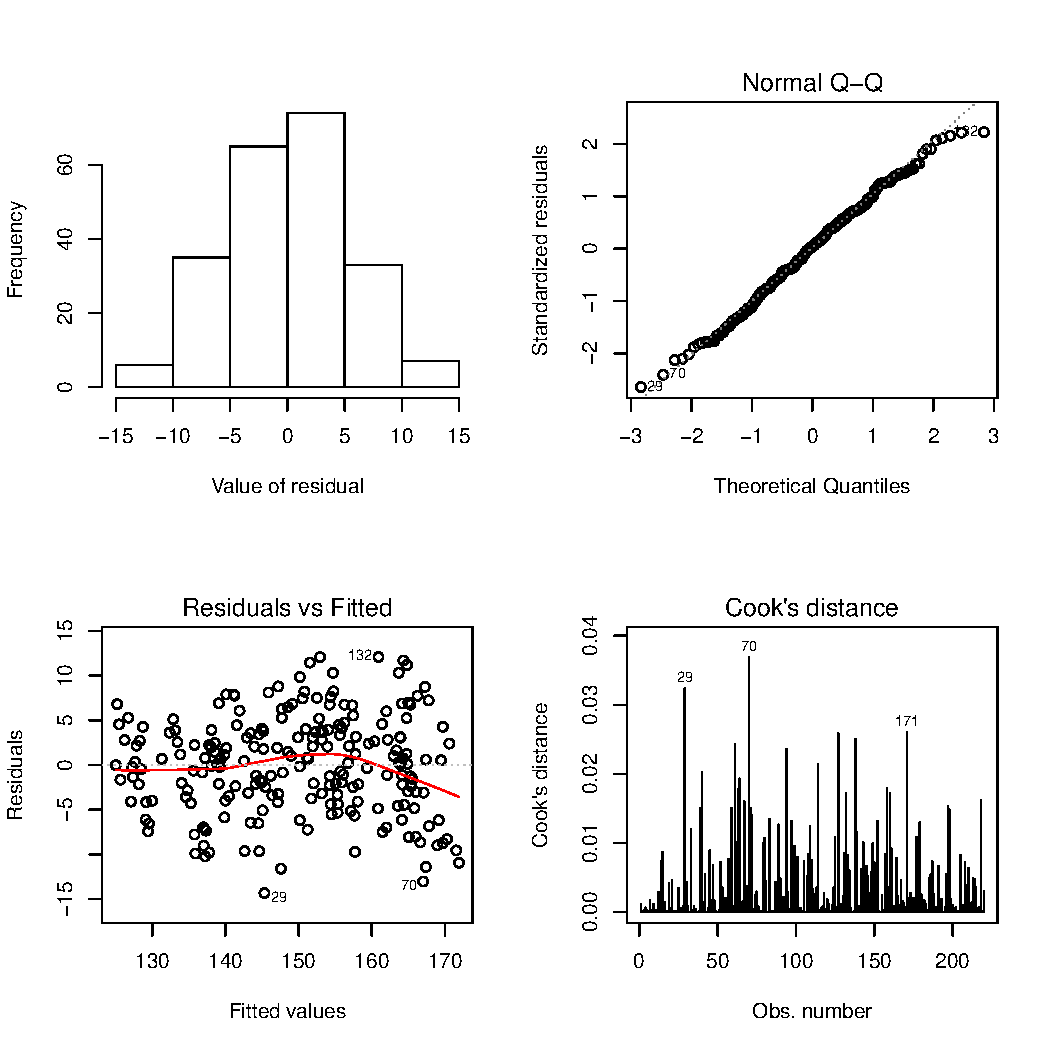
\includegraphics[width=\maxwidth]{figure/unnamed-chunk-44-1} 
\begin{kframe}\begin{alltt}
\hlcom{# Focusing only on departure delay < 400 mins for more readable plot}
\end{alltt}
\end{kframe}
\end{knitrout}
\caption{Scatter plot of Arrival Delay vs Departure Delay}
\label{Fig:scatter}
\rule{4in}{1pt}
\end{figure}

What we essentially want to do is to draw a line through the Figure: \ref{Fig:scatter} such that the line represents all the scatter points well. There are several ways of drawing this line. The most popular method is called OLS (Ordinary Least Square) that draws a line such that the sum of the square of distances (called \textbf{residuals} \index{Key Concepts!Residuals} between the line and all the points is minimized. This method is commonly known as linear regression. 

We can now formalize the relationship between the two variables by running a \textbf{Linear Regression}. Recall that a linear regression essentially involves modeling the relationship between a predictor variable ($x$) and a response variable ($y$) as follows: $y_i = \beta_0 + \beta_1 x_i + \epsilon_i$. This is similar to plotting a line with a $y$ intercept of $\beta_0$ and the $\beta_1$ as the slope of the line. Through OLS Linear Regression we are trying to estimate the values of $\beta$s. Further, to ensure that the analysis is robust and applicable, we are also looking to check whether a) the model itself is statistically significant and b) the coefficients are statistically significant. 

The term \textbf{Statistically Significant} \index{Key Concepts!Statistical Significance} has a specific meaning here. It means that we can reject the null hypothesis of no effect with more than 95\% (or any other level you choose, the default is 95\%) confidence. That means that the probability that what we are observing is because of pure chance and randomness is less than 5\%. Note that the probability of the analysis being flat out wrong is non-zero. That's why we need to be careful in interpreting the results of a regression analysis.

We can run the linear regression using the \texttt{lm()} \index{R Commands!lm} command.
\begin{knitrout}
\definecolor{shadecolor}{rgb}{0.969, 0.969, 0.969}\color{fgcolor}\begin{kframe}
\begin{alltt}
\hlstd{m} \hlkwb{<-} \hlkwd{lm}\hlstd{(arr_delay} \hlopt{~} \hlstd{dep_delay)}
\end{alltt}
\end{kframe}
\end{knitrout}

We have saved the result of the model in the object \texttt{m}. We can now extract relevant information from this object. \index{R Commands!coef}\index{R Commands!confint}
\begin{knitrout}
\definecolor{shadecolor}{rgb}{0.969, 0.969, 0.969}\color{fgcolor}\begin{kframe}
\begin{alltt}
\hlkwd{coef}\hlstd{(m)}  \hlcom{#provides coefficients}
\end{alltt}
\begin{verbatim}
## (Intercept)   dep_delay 
##   -4.057010    1.020178
\end{verbatim}
\begin{alltt}
\hlkwd{confint}\hlstd{(m)}  \hlcom{#provides confidence interval for the coefficients}
\end{alltt}
\begin{verbatim}
##                 2.5 %    97.5 %
## (Intercept) -4.259533 -3.854486
## dep_delay    1.014800  1.025556
\end{verbatim}
\end{kframe}
\end{knitrout}

Now that we know the coefficients, we can now draw the fitted line that models the relationship between Arrival Delay and Departure Delay \index{R Commands!abline} as shown in Figure \ref{fig:fitted}. This is the same line we described in our earlier discussion of OLS - this line minimizes the sum of the squares of the distance between all the points and this line. 

\begin{figure}
\centering
\rule{4in}{1pt}
\begin{knitrout}
\definecolor{shadecolor}{rgb}{0.969, 0.969, 0.969}\color{fgcolor}\begin{kframe}
\begin{alltt}
\hlkwd{plot}\hlstd{(}\hlkwc{x} \hlstd{= dep_delay[dep_delay} \hlopt{<} \hlnum{400}\hlstd{],} \hlkwc{y} \hlstd{= arr_delay[dep_delay} \hlopt{<} \hlnum{400}\hlstd{],} \hlkwc{xlab} \hlstd{=} \hlstr{"Departure Delay"}\hlstd{,}
    \hlkwc{ylab} \hlstd{=} \hlstr{"Arrival Delay"}\hlstd{)}
\hlkwd{abline}\hlstd{(}\hlkwd{coef}\hlstd{(m),} \hlkwc{lwd} \hlstd{=} \hlnum{2}\hlstd{,} \hlkwc{col} \hlstd{=} \hlstr{"red"}\hlstd{)}
\end{alltt}
\end{kframe}
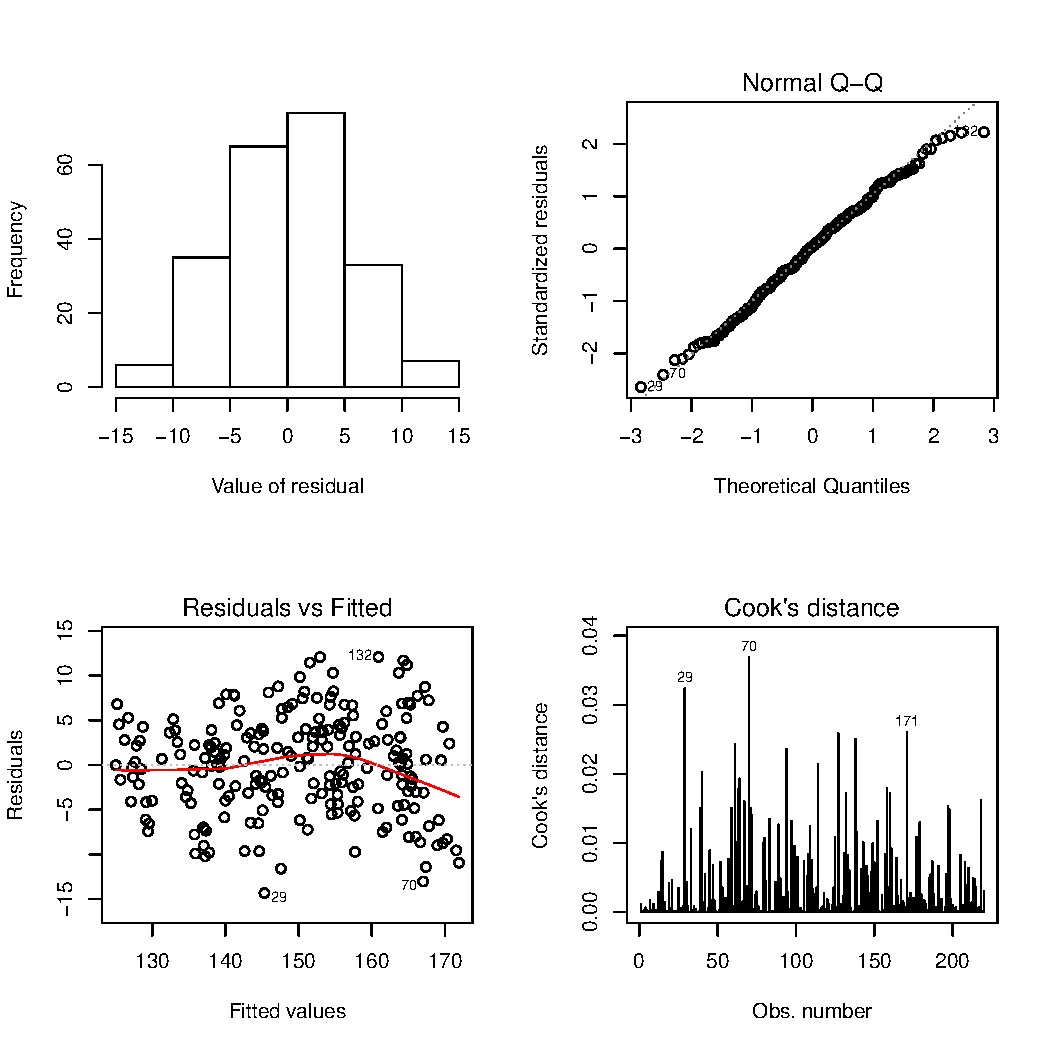
\includegraphics[width=\maxwidth]{figure/unnamed-chunk-47-1} 

\end{knitrout}
\caption{Plotting Fitted Values of Regression Model}
\label{fig:fitted}
\rule{4in}{1pt}
\end{figure}

As you can see that the line is not a perfect fit for all the points. The model provides a handy statistics called the Coefficient of Determination or the R-Square \index{Key Concepts!R-Square} to check just how good of a fit the line actually is. To get R-Square and other useful information, we can use the command \textbf(summary) \index{R Commands!summary} provides a good balanced amount of details.

\begin{knitrout}
\definecolor{shadecolor}{rgb}{0.969, 0.969, 0.969}\color{fgcolor}\begin{kframe}
\begin{alltt}
\hlkwd{summary}\hlstd{(m)}
\end{alltt}
\begin{verbatim}
## 
## Call:
## lm(formula = arr_delay ~ dep_delay)
## 
## Residuals:
##     Min      1Q  Median      3Q     Max 
## -65.185  -9.903  -1.024   9.057 132.371 
## 
## Coefficients:
##              Estimate Std. Error t value Pr(>|t|)    
## (Intercept) -4.057010   0.103326  -39.26   <2e-16 ***
## dep_delay    1.020178   0.002744  371.80   <2e-16 ***
## ---
## Signif. codes:  0 '***' 0.001 '**' 0.01 '*' 0.05 '.' 0.1 ' ' 1
## 
## Residual standard error: 16.19 on 26396 degrees of freedom
##   (606 observations deleted due to missingness)
## Multiple R-squared:  0.8397,	Adjusted R-squared:  0.8397 
## F-statistic: 1.382e+05 on 1 and 26396 DF,  p-value: < 2.2e-16
\end{verbatim}
\end{kframe}
\end{knitrout}

Important things to note here is that the model itself has a \textbf{p-value} \index{Key Concepts!p-value} of close to zero. p-value can be interpreted as the probability of something happening by chance, by randomness. So first thing we see is that the probability of us getting this result by chance is virtually nil. So that's a good start. 

Now we see that the p-value for the coefficient of Departure Delay (or $\beta_1$) in our model is again close to zero. This means that the probability that the predictor (in this case Departure Delay) has no impact (in other words $\beta_1 = 0$) on the response (in this case Arrival Delay) is close to zero as well. So we can conclude that Departure Delay has a statistically significant relationship with Arrival Delay. As the value of the coefficient is 1.02, we can conclude that, on an average, each minute of Departure Delay increases the Arrival Delay by 1.02 minutes.

Finally, the model has an R-Square of 0.8397. This can be interpreted as a goodness-of-fit indicator. We can say that the model explains 83.97\% of the variance in the response variable. The R-Square value is susceptible to number of predictor variables - adding more predictor variables, even if they are not significant, increases the R-Square value. To correct for this over-estimation, the Adjusted R-Square \index{Key Concepts!Adjusted R-Square} can be used instead. As the model summary shows, the Adjusted R-Square value is same as R-Square value as we have only one predictor variable right now.

\subsection{Multiple Regression}

The basic concept of OLS Linear Regression can be easily extended to more than one predictor variables. For illustration, lets look at the following dataset that has measurement of Systolic Blood Pressure, Age (in years) and Weight (in lbs) for patients.

\begin{knitrout}
\definecolor{shadecolor}{rgb}{0.969, 0.969, 0.969}\color{fgcolor}\begin{kframe}
\begin{alltt}
\hlstd{bp} \hlkwb{<-} \hlkwd{read.csv}\hlstd{(}\hlstr{"bp.csv"}\hlstd{)}
\end{alltt}
\end{kframe}
\end{knitrout}

We can consider that Blood Pressure of a patient is a function of Age of patient and Weight of patient. So we can specify the following linear regression model.

\begin{knitrout}
\definecolor{shadecolor}{rgb}{0.969, 0.969, 0.969}\color{fgcolor}\begin{kframe}
\begin{alltt}
\hlstd{bpmodel} \hlkwb{<-} \hlkwd{lm}\hlstd{(bp} \hlopt{~} \hlstd{age} \hlopt{+} \hlstd{weight,} \hlkwc{data} \hlstd{= bp)}
\hlkwd{summary}\hlstd{(bpmodel)}
\end{alltt}
\begin{verbatim}
## 
## Call:
## lm(formula = bp ~ age + weight, data = bp)
## 
## Residuals:
##      Min       1Q   Median       3Q      Max 
## -14.3233  -3.6146   0.1924   3.8740  12.0820 
## 
## Coefficients:
##             Estimate Std. Error t value Pr(>|t|)    
## (Intercept) 42.27980    4.75515   8.891 2.38e-16 ***
## age          0.94348    0.08792  10.731  < 2e-16 ***
## weight       0.25135    0.04526   5.553 8.16e-08 ***
## ---
## Signif. codes:  0 '***' 0.001 '**' 0.01 '*' 0.05 '.' 0.1 ' ' 1
## 
## Residual standard error: 5.457 on 217 degrees of freedom
## Multiple R-squared:  0.8394,	Adjusted R-squared:  0.8379 
## F-statistic: 567.1 on 2 and 217 DF,  p-value: < 2.2e-16
\end{verbatim}
\end{kframe}
\end{knitrout}

We can see in the model summary results that the model itself - our argument that a patient's age and weight have a significant relationship with patient's blood pressure - is indeed statistically significant (model p-value < 0.05). The coefficients of our two predictor variables are statistically significant as well with p-value for both coefficients < 0.05. We can interpret that for each year's increase in age, blood pressure rises by 0.94 points. Further, for each lbs increase in weight, blood pressure increases by 0.25. These two predictor variables explain about 84\% of the variance in blood pressure as shown by the R-Square value.

\subsection{Prediction Based on Regression Model}

Once we have a model, we can use the model to predict new values. If, for example, a person is of 60 years age and 140 lb weight, we can predict corresponding blood pressure. We can get either a point prediction or an interval prediction corresponding to a confidence interval.

\begin{knitrout}
\definecolor{shadecolor}{rgb}{0.969, 0.969, 0.969}\color{fgcolor}\begin{kframe}
\begin{alltt}
\hlstd{newvalue} \hlkwb{<-} \hlkwd{data.frame}\hlstd{(}\hlkwc{age} \hlstd{=} \hlnum{50}\hlstd{,} \hlkwc{weight} \hlstd{=} \hlnum{150}\hlstd{)}
\hlcom{# A Point Prediction}
\hlkwd{predict}\hlstd{(bpmodel,} \hlkwc{newdata} \hlstd{= newvalue)}
\end{alltt}
\begin{verbatim}
##        1 
## 127.1567
\end{verbatim}
\begin{alltt}
\hlcom{# Confidence Interval}
\hlkwd{predict}\hlstd{(bpmodel,} \hlkwc{newdata} \hlstd{= newvalue,} \hlkwc{interval} \hlstd{=} \hlstr{"confidence"}\hlstd{)}
\end{alltt}
\begin{verbatim}
##        fit      lwr      upr
## 1 127.1567 124.7148 129.5985
\end{verbatim}
\begin{alltt}
\hlcom{# Prediction Interval}
\hlkwd{predict}\hlstd{(bpmodel,} \hlkwc{newdata} \hlstd{= newvalue,} \hlkwc{interval} \hlstd{=} \hlstr{"prediction"}\hlstd{)}
\end{alltt}
\begin{verbatim}
##        fit      lwr      upr
## 1 127.1567 116.1275 138.1858
\end{verbatim}
\end{kframe}
\end{knitrout}

As the results show, a person with age 50 years and weight 150 years is predicted to have a blood pressure value of 127.16. This is the point estimate. The 95\% confidence interval for the mean blood pressure value is 124.71 - 129.60. The 95\% prediction interval for the point estimate is 116.13 - 138.19. 

\section{Regression Diagnostics}

OLS Regression depends on the underlying data following several assumptions. If these conditions are not met then regression results need to be further investigated as they may not be accurate. Following are the key requirements:

\subsection{Normality}

Like much of Statistics, OLS works best with data that follows Normal Distribution. Specifically, linear regression assumes that the residuals are normally distributed. The residuals are assumed to be independent and with a mean of zero.

We can plot residuals to check their normality. See Figure: \ref{Fig:residuals} for four such plots. First plot is a histogram of residuals - looks pretty well distributed for our case. Second plot is a Q-Q Plot of residuals - again we see that residuals stick to the normal line very well. Plot 3 shows residuals against fitted values while Plot 4 shows Cook's Distance. Visual inspection of these charts does not show specific patterns that may violate normality of residuals. We will use Cook's Distance plot in our discussion of outliers in coming sections.

\begin{figure}
\centering
\rule{4in}{1pt}
\begin{knitrout}
\definecolor{shadecolor}{rgb}{0.969, 0.969, 0.969}\color{fgcolor}\begin{kframe}
\begin{alltt}
\hlkwd{par}\hlstd{(}\hlkwc{mfrow} \hlstd{=} \hlkwd{c}\hlstd{(}\hlnum{2}\hlstd{,} \hlnum{2}\hlstd{))}
\hlkwd{hist}\hlstd{(}\hlkwc{x} \hlstd{=} \hlkwd{residuals}\hlstd{(bpmodel),} \hlkwc{xlab} \hlstd{=} \hlstr{"Value of residual"}\hlstd{,} \hlkwc{main} \hlstd{=} \hlstr{""}\hlstd{)}
\hlkwd{plot}\hlstd{(}\hlkwc{x} \hlstd{= bpmodel,} \hlkwc{which} \hlstd{=} \hlnum{2}\hlstd{)}  \hlcom{#QQ Plot}
\hlkwd{plot}\hlstd{(}\hlkwc{x} \hlstd{= bpmodel,} \hlkwc{which} \hlstd{=} \hlnum{1}\hlstd{)}  \hlcom{#Residuals vs Fitted}
\hlkwd{plot}\hlstd{(}\hlkwc{x} \hlstd{= bpmodel,} \hlkwc{which} \hlstd{=} \hlnum{4}\hlstd{)}  \hlcom{#Cook's Distance}
\end{alltt}
\end{kframe}
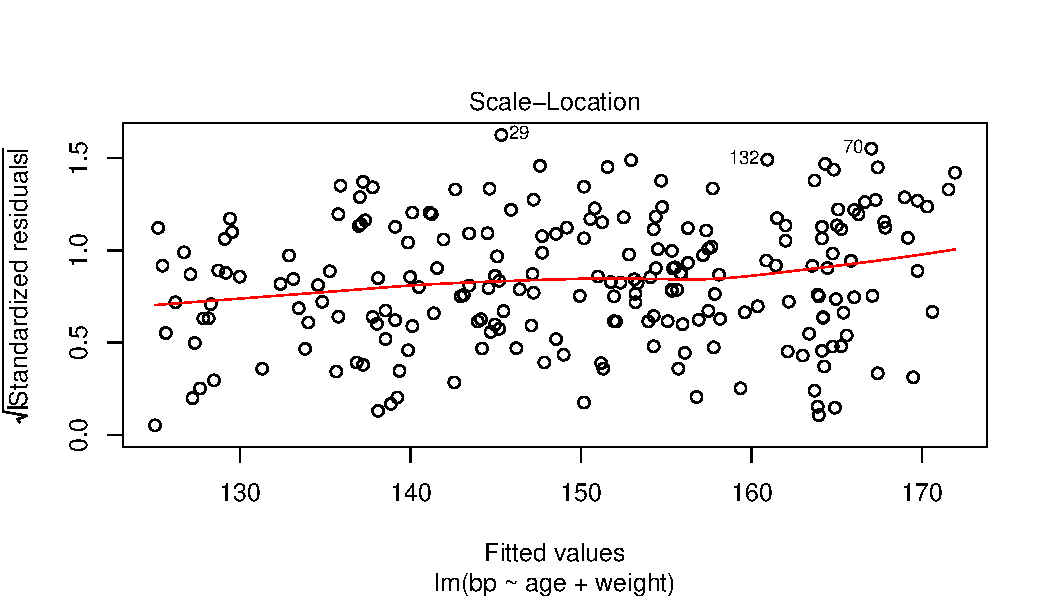
\includegraphics[width=\maxwidth]{figure/unnamed-chunk-52-1} 

\end{knitrout}
\caption{Histogram of Residuals}
\label{Fig:residuals}
\rule{4in}{1pt}
\end{figure}

We can also use the Shapiro-Wilk Normality test \index{R Commands!shapiro.test} as shown below:

\begin{knitrout}
\definecolor{shadecolor}{rgb}{0.969, 0.969, 0.969}\color{fgcolor}\begin{kframe}
\begin{alltt}
\hlkwd{shapiro.test}\hlstd{(}\hlkwd{residuals}\hlstd{(bpmodel))}
\end{alltt}
\begin{verbatim}
## 
## 	Shapiro-Wilk normality test
## 
## data:  residuals(bpmodel)
## W = 0.9934, p-value = 0.4379
\end{verbatim}
\end{kframe}
\end{knitrout}

We can see that the null hypothesis of normality was not rejected as the p-value > 0.05. So we can conclude that the assumption of normality is satisfied in our model. 

\subsection{Linearity}

As the name suggests, we are only exploring linear relationships between predictors and the response variable. A good graphical way to explore linearity is to check the plots created by the \texttt{residualPlots()} \index{R Commands!residualPlots} function in the \texttt{car} \index{Packages!car} package. As Figure: \ref{Fig:linear} suggests, weight seems to have a straight linear relationship with. Age, however, shows some curvature that can be further explored.



\begin{figure}
\centering
\rule{4in}{1pt}
\begin{knitrout}
\definecolor{shadecolor}{rgb}{0.969, 0.969, 0.969}\color{fgcolor}\begin{kframe}
\begin{alltt}
\hlkwd{residualPlots}\hlstd{(bpmodel)}
\end{alltt}
\end{kframe}
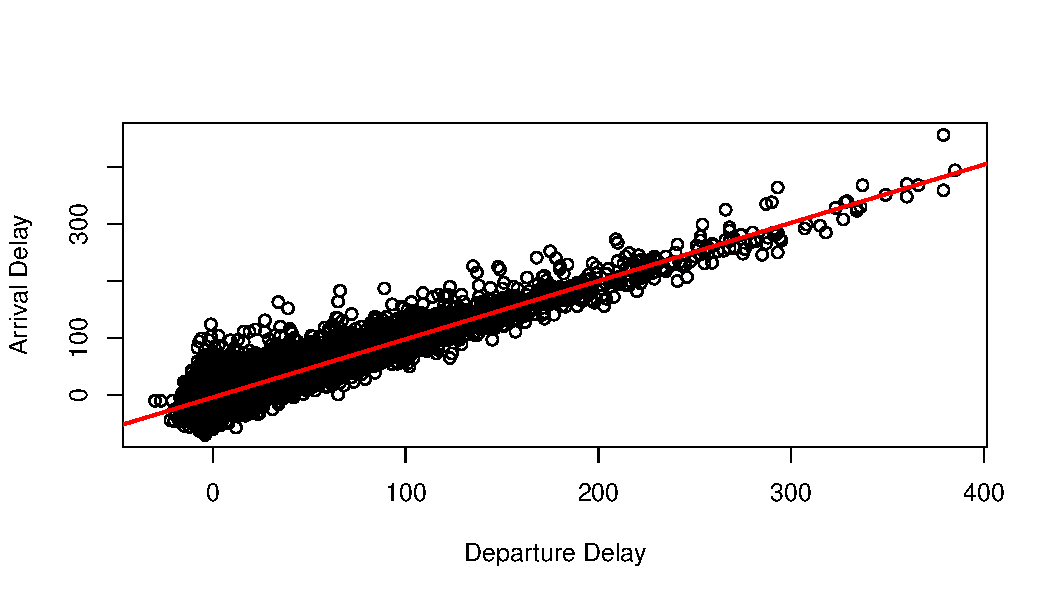
\includegraphics[width=\maxwidth]{figure/unnamed-chunk-55-1} 
\begin{kframe}\begin{verbatim}
##            Test stat Pr(>|t|)
## age           -3.251    0.001
## weight        -0.262    0.794
## Tukey test    -2.359    0.018
\end{verbatim}
\end{kframe}
\end{knitrout}
\caption{Plots to Check Linearity}
\label{Fig:linear}
\rule{4in}{1pt}
\end{figure}

It is important to note that OLS only needs residuals to be normal. Predictor variables need not be distributed normally. This allows us to do nearly limitless data transformation (taking square, cube, square-root, log etc.) and still meet the linearity assumption. For example, we could very well have run a regression analysis with log transformed values of age and weight as predictor variables.

\begin{knitrout}
\definecolor{shadecolor}{rgb}{0.969, 0.969, 0.969}\color{fgcolor}\begin{kframe}
\begin{alltt}
\hlstd{newbp} \hlkwb{<-} \hlkwd{lm}\hlstd{(bp} \hlopt{~} \hlkwd{log}\hlstd{(age)} \hlopt{+} \hlkwd{log}\hlstd{(weight),} \hlkwc{data} \hlstd{= bp)}
\hlkwd{summary}\hlstd{(newbp)}
\end{alltt}
\begin{verbatim}
## 
## Call:
## lm(formula = bp ~ log(age) + log(weight), data = bp)
## 
## Residuals:
##      Min       1Q   Median       3Q      Max 
## -15.0462  -3.8825   0.4448   3.5703  12.0816 
## 
## Coefficients:
##             Estimate Std. Error t value Pr(>|t|)    
## (Intercept) -338.664     28.593 -11.844  < 2e-16 ***
## log(age)      57.062      5.272  10.823  < 2e-16 ***
## log(weight)   48.124      8.727   5.515 9.89e-08 ***
## ---
## Signif. codes:  0 '***' 0.001 '**' 0.01 '*' 0.05 '.' 0.1 ' ' 1
## 
## Residual standard error: 5.393 on 217 degrees of freedom
## Multiple R-squared:  0.8432,	Adjusted R-squared:  0.8417 
## F-statistic: 583.3 on 2 and 217 DF,  p-value: < 2.2e-16
\end{verbatim}
\end{kframe}
\end{knitrout}

Key here is to build a model that is theoretically consistent. Running a regression analysis and getting a bunch of coefficients is the easy part - the hard part is to design a model in the first place that makes sense. As they say - Correlation is not Causation. Just because a model is statistically significant, it does not mean that the model is also correct.

\subsection{Homegeniety of Variance}

The OLS model assumes that all the residuals have a constant variance. It is conventional to look at the plot in Figure: \ref{Fig:variance} to check for potential heterogeneity in the model, also called heteroscedasticity. As the plot show, there is small trend in the residuals but it may not be significant.

\begin{figure}
\centering
\rule{4in}{1pt}
\begin{knitrout}
\definecolor{shadecolor}{rgb}{0.969, 0.969, 0.969}\color{fgcolor}\begin{kframe}
\begin{alltt}
\hlkwd{plot}\hlstd{(}\hlkwc{x} \hlstd{= bpmodel,} \hlkwc{which} \hlstd{=} \hlnum{3}\hlstd{)}
\end{alltt}
\end{kframe}
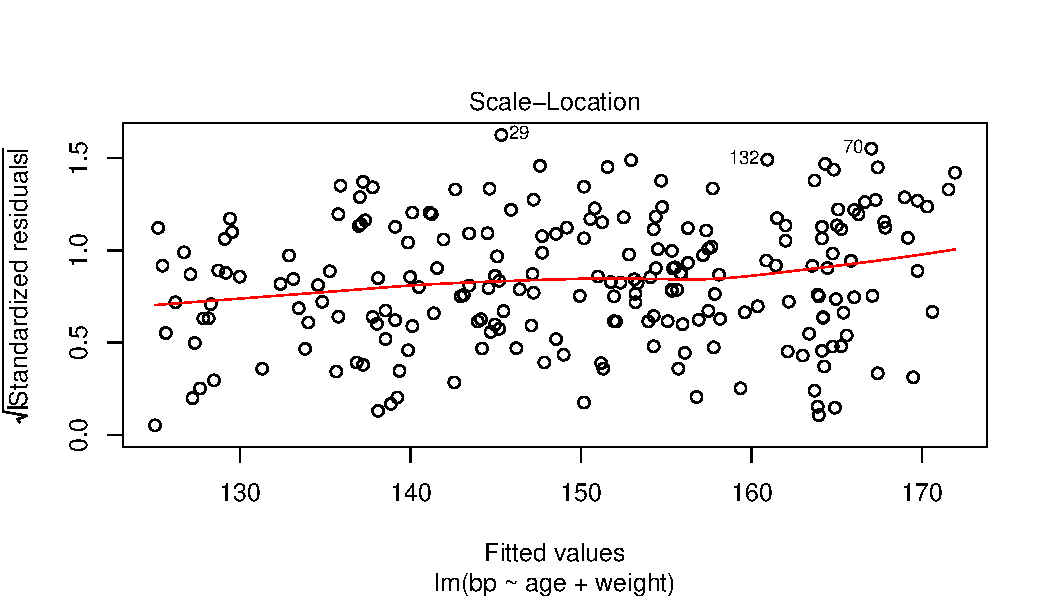
\includegraphics[width=\maxwidth]{figure/unnamed-chunk-57-1} 

\end{knitrout}
\caption{Plot to Check for Heteroscedasticity}
\label{Fig:variance}
\rule{4in}{1pt}
\end{figure}

We can further explore the possibility of heteroscedasticity by using the Breuch Pagan test available as the \texttt{bptest()} \index{R Commands!bptest} function in the \texttt{lmtest} \index{Packages!lmtest} package. 



\begin{knitrout}
\definecolor{shadecolor}{rgb}{0.969, 0.969, 0.969}\color{fgcolor}\begin{kframe}
\begin{alltt}
\hlkwd{bptest}\hlstd{(bpmodel)}
\end{alltt}
\begin{verbatim}
## 
## 	studentized Breusch-Pagan test
## 
## data:  bpmodel
## BP = 7.83, df = 2, p-value = 0.01994
\end{verbatim}
\end{kframe}
\end{knitrout}

The Breuch Pagan test tests the null hypothesis of no heteroscedasticity. As can be seen from the results, the null hypothesis is rejected at 95\% confidence interval and we do \textbf{not} have constant variance of residuals in our model.

\subsection{Uncorrelated Predictors}

The OLS model assumes that the predictor variables are independent and not related to each other. Any significant correlation between predictor variables would make the model results less reliable. Correlation between predictor variables, called MultiCollinearity \index{Key Concepts!Multicollinearity} can be estimated using Variance Inflation Factors. Variance Inflation Factors can be calculated using the \texttt{vif()} \index{R Commands!vif} function. A VIF value less than 10 is considered acceptable.

\begin{knitrout}
\definecolor{shadecolor}{rgb}{0.969, 0.969, 0.969}\color{fgcolor}\begin{kframe}
\begin{alltt}
\hlkwd{vif}\hlstd{(bpmodel)}
\end{alltt}
\begin{verbatim}
##     age  weight 
## 4.51628 4.51628
\end{verbatim}
\end{kframe}
\end{knitrout}

We can see from the output above that correlations between predictor variables is not a concern in our model.

\subsection{Independent Residuals}

We can if residuals are correlated with each other using the Durbin-Watson test. This test is available as function \texttt{dwtest} as part of the \texttt{lmtest} package. Like the Breuch Pagan test, this test looks at null hypothesis of no autocorrelation and tries to reject it. A p-value > 0.05 shows that the null hypothesis could not be rejected and we do not have statistically significant evidence of autocorrelation.

\begin{knitrout}
\definecolor{shadecolor}{rgb}{0.969, 0.969, 0.969}\color{fgcolor}\begin{kframe}
\begin{alltt}
\hlkwd{dwtest}\hlstd{(bpmodel)}
\end{alltt}
\begin{verbatim}
## 
## 	Durbin-Watson test
## 
## data:  bpmodel
## DW = 2.1197, p-value = 0.8192
## alternative hypothesis: true autocorrelation is greater than 0
\end{verbatim}
\end{kframe}
\end{knitrout}

\subsection{Outliers}

Outlier values are those that differ greatly from other values of predictors or the response variables. Outliers can skew the regression line and can have significant influence on the regression results. Outliers can be visually detected in various diagnostic plots we have done so far. Formal detection of outliers usually considers two approaches: Leverage and Influence. Leverage statistics are designed to identify observations which have predictor values that are far away from the rest of the data. Influence statistics look at which values play too large a role in the regression model.

We can measure the change in the regression results as a result of deleting an observation. This value is called \texttt{DFBETAs}. It can be calculated using the \texttt{dfbetas} \index{R Commands!dfbetas} function.

\begin{knitrout}
\definecolor{shadecolor}{rgb}{0.969, 0.969, 0.969}\color{fgcolor}\begin{kframe}
\begin{alltt}
\hlstd{dfb} \hlkwb{<-} \hlkwd{dfbetas}\hlstd{(bpmodel)}
\hlkwd{head}\hlstd{(dfb)}
\end{alltt}
\begin{verbatim}
##    (Intercept)           age       weight
## 1 -0.039521410  0.0040605801  0.017320382
## 2 -0.011804765 -0.0053884549  0.009100589
## 3 -0.010800476 -0.0186179048  0.016753416
## 4  0.010021037 -0.0212482412  0.006672112
## 5  0.003553237  0.0065673756 -0.004930005
## 6 -0.008912326  0.0003038909  0.004934012
\end{verbatim}
\end{kframe}
\end{knitrout}

Output above shows that the first data point, if removed, will change the intercept by $-0.039$. Similarly We can measure the influence that an observation has on its fitted value with the function \texttt{dffits}. \index{R Commands!dffits} DFFITS can be interpreted in the same way as DFBETAS.

\begin{knitrout}
\definecolor{shadecolor}{rgb}{0.969, 0.969, 0.969}\color{fgcolor}\begin{kframe}
\begin{alltt}
\hlstd{dff} \hlkwb{<-} \hlkwd{dffits}\hlstd{(bpmodel)}
\hlkwd{head}\hlstd{(dff)}
\end{alltt}
\begin{verbatim}
##           1           2           3           4           5           6 
## -0.05685922 -0.01827616 -0.02433017 -0.04307776  0.02656855  0.01340052
\end{verbatim}
\end{kframe}
\end{knitrout}

While the DFFITS are good for measuring the influence on a single fitted value, Cook's Distance measures the influence an observation on all of the fitted values simultaneously. We saw a plot of Cook's Distance in \ref{Fig:residuals}. We can also generate Cook's Distance values using the \texttt{cooks.distance} function. \index{R Commands!cooks.distance}
\begin{knitrout}
\definecolor{shadecolor}{rgb}{0.969, 0.969, 0.969}\color{fgcolor}\begin{kframe}
\begin{alltt}
\hlstd{cooksd} \hlkwb{<-} \hlkwd{cooks.distance}\hlstd{(bpmodel)}
\hlkwd{head}\hlstd{(cooksd)}
\end{alltt}
\begin{verbatim}
##            1            2            3            4            5 
## 1.081293e-03 1.118300e-04 1.981837e-04 6.209621e-04 2.362273e-04 
##            6 
## 6.013163e-05
\end{verbatim}
\end{kframe}
\end{knitrout}

We can also formally test for outliers using the \texttt{outlierTest()} \index{R Commands!outlierTest} function in the \texttt{car} package.

\begin{knitrout}
\definecolor{shadecolor}{rgb}{0.969, 0.969, 0.969}\color{fgcolor}\begin{kframe}
\begin{alltt}
\hlkwd{outlierTest}\hlstd{(bpmodel)}
\end{alltt}
\begin{verbatim}
## 
## No Studentized residuals with Bonferonni p < 0.05
## Largest |rstudent|:
##    rstudent unadjusted p-value Bonferonni p
## 29 -2.68033          0.0079222           NA
\end{verbatim}
\end{kframe}
\end{knitrout}

This function identifies significant outliers. As we can see, our current dataset does not have any significant outliers. However, there still would be observations that will have more influence on the model than other. These influential observations can be identified using the \texttt{influence.measure()} \index{R Commands!influence.measure} function.

\begin{knitrout}
\definecolor{shadecolor}{rgb}{0.969, 0.969, 0.969}\color{fgcolor}\begin{kframe}
\begin{alltt}
\hlkwd{influence.measures}\hlstd{(bpmodel)}  \hlcom{#Output removed to save space}
\end{alltt}
\end{kframe}
\end{knitrout}

\section{Improving Regression Model}

In this section we will explore various techniques for building the most appropriate regression model. We will start by checking how we can specify our model to have higher order variables like square of values.

\subsection{Polynomial Regression}

We will consider a new dataset called $trees$ for this portion. The dataset has the following columns: $Volume$, $Girth$ and $Height$. Here $Volume$ is the response variable and $Girth$ and $Height$ are the predictor variables. We can quickly explore this data by building a scatterplot shown in Figure: \ref{Fig:trees}.

\begin{figure}
\centering
\rule{4in}{1pt}
\begin{knitrout}
\definecolor{shadecolor}{rgb}{0.969, 0.969, 0.969}\color{fgcolor}\begin{kframe}
\begin{alltt}
\hlkwd{attach}\hlstd{(trees)}
\hlkwd{plot}\hlstd{(Girth, Volume)}
\end{alltt}
\end{kframe}
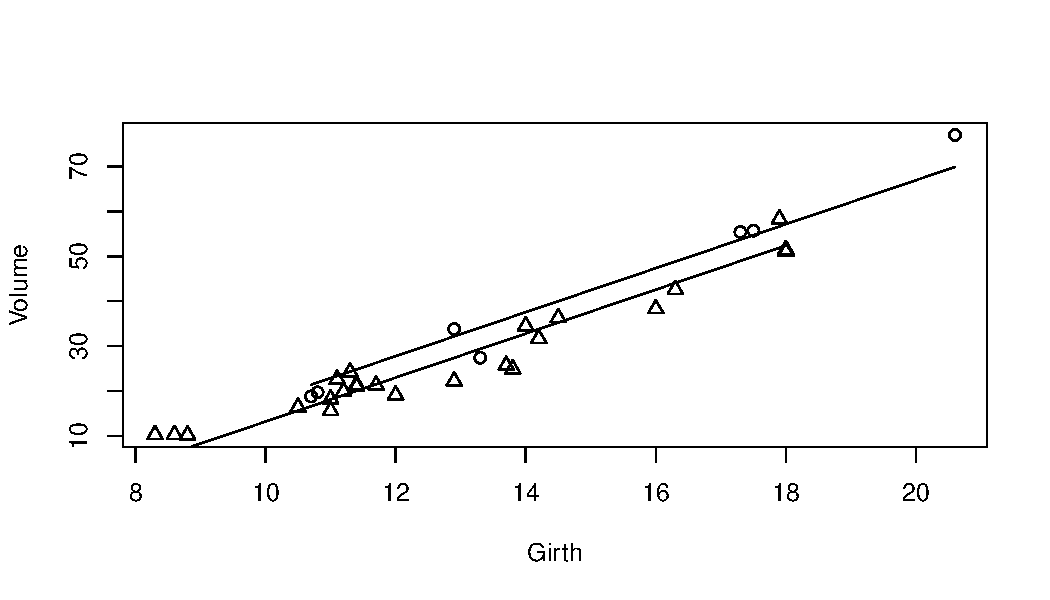
\includegraphics[width=\maxwidth]{figure/unnamed-chunk-67-1} 

\end{knitrout}
\caption{Volume vs Girth of Tree Trunks}
\label{Fig:trees}
\rule{4in}{1pt}
\end{figure}

As we can see, the data does not seem linear. Values towards the right are curving upwards. We can try to capture this non-linear effect by specifying a square term in the model as follows: $ y = \beta_0 + \beta_1 x_1 + \beta_1 x_1^2 + \epsilon $. However, including a square term usually adds a large dose of multicollinearity (correlation between predictor variables) to the model. To reduce the negative impact of multicollinearity, it is suggested that data should be standardized - rescaled to have a mean = 0. We can do this in R as follows:
\begin{knitrout}
\definecolor{shadecolor}{rgb}{0.969, 0.969, 0.969}\color{fgcolor}\begin{kframe}
\begin{alltt}
\hlstd{treemodel} \hlkwb{<-} \hlkwd{lm}\hlstd{(Volume} \hlopt{~} \hlkwd{scale}\hlstd{(Girth)} \hlopt{+} \hlkwd{I}\hlstd{(}\hlkwd{scale}\hlstd{(Girth)}\hlopt{^}\hlnum{2}\hlstd{))}
\hlkwd{summary}\hlstd{(treemodel)}
\end{alltt}
\begin{verbatim}
## 
## Call:
## lm(formula = Volume ~ scale(Girth) + I(scale(Girth)^2))
## 
## Residuals:
##     Min      1Q  Median      3Q     Max 
## -5.4889 -2.4293 -0.3718  2.0764  7.6447 
## 
## Coefficients:
##                   Estimate Std. Error t value Pr(>|t|)    
## (Intercept)        27.7452     0.8161  33.996  < 2e-16 ***
## scale(Girth)       14.5995     0.6773  21.557  < 2e-16 ***
## I(scale(Girth)^2)   2.5067     0.5729   4.376 0.000152 ***
## ---
## Signif. codes:  0 '***' 0.001 '**' 0.01 '*' 0.05 '.' 0.1 ' ' 1
## 
## Residual standard error: 3.335 on 28 degrees of freedom
## Multiple R-squared:  0.9616,	Adjusted R-squared:  0.9588 
## F-statistic: 350.5 on 2 and 28 DF,  p-value: < 2.2e-16
\end{verbatim}
\end{kframe}
\end{knitrout}

Results show that both $Girth$ and $Girth^2$ have significant coefficients. The model is strongly significant as well and has a very high R-Square value. We can graphically see the how model fits in Figure: \ref{Fig:quadtrees}. As we can see, the model fits the data very well.

\begin{figure}
\centering
\rule{4in}{1pt}
\begin{knitrout}
\definecolor{shadecolor}{rgb}{0.969, 0.969, 0.969}\color{fgcolor}\begin{kframe}
\begin{alltt}
\hlkwd{plot}\hlstd{(}\hlkwd{scale}\hlstd{(Girth), Volume)}
\hlkwd{lines}\hlstd{(}\hlkwd{fitted}\hlstd{(treemodel)} \hlopt{~} \hlkwd{scale}\hlstd{(Girth))}
\end{alltt}
\end{kframe}
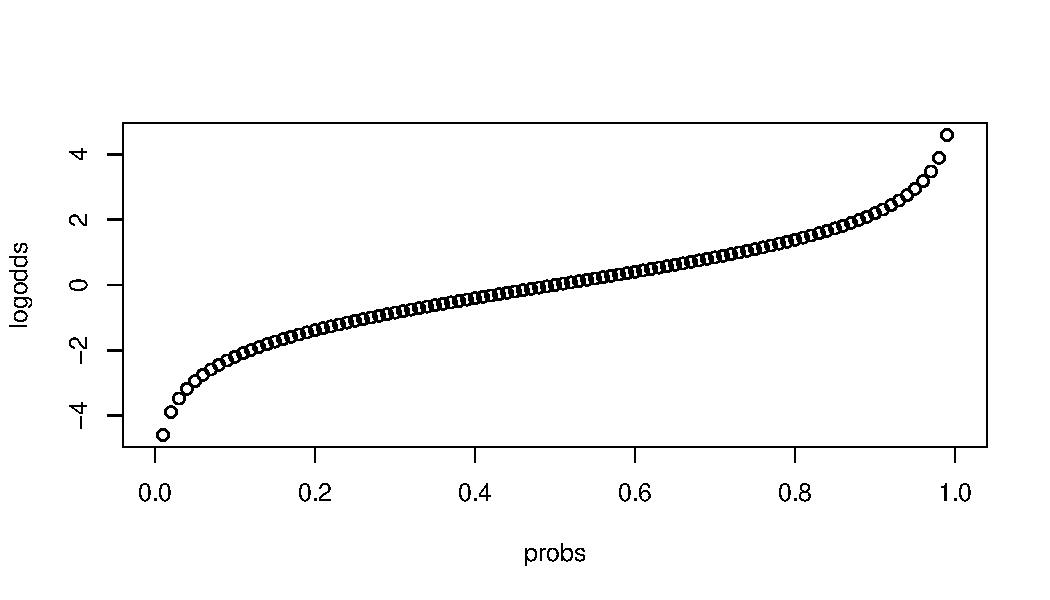
\includegraphics[width=\maxwidth]{figure/unnamed-chunk-69-1} 

\end{knitrout}
\caption{Quadratic Model of Volume vs Girth of Tree Trunks}
\label{Fig:quadtrees}
\rule{4in}{1pt}
\end{figure}

When including higher order variables, we should be mindful of the principle of \texttt{parsimony} \index{Key Concepts!Parsimony} which states that if a higher order term $x^m$ is part of the model then all lower order terms $x$, $x^2$ through $x^{m-1}$ should be part of the model as well.

\subsection{Interaction Between Predictors}

Even though predictor variables are assumed to be independent of each other, they may interact in their influence on the response variable. That is - the impact of one predictor variable in the response variable may depend on the value of a different predictor variable.  We can capture such interaction effects by including an additional term in our model. Such interaction terms are usually formed by multiplying one predictor variable by another. This results in model specifications like: $y = \beta_0 + \beta_1 x_1 + \beta_2 x_2 + \beta_{1:2} x_1 x_2 + \epsilon$ where $\beta_{1:2}$ indicate a coefficient of an interaction term. We can do this in R as follows:

\begin{knitrout}
\definecolor{shadecolor}{rgb}{0.969, 0.969, 0.969}\color{fgcolor}\begin{kframe}
\begin{alltt}
\hlstd{treeint} \hlkwb{<-} \hlkwd{lm}\hlstd{(Volume} \hlopt{~} \hlstd{Girth} \hlopt{+} \hlstd{Height} \hlopt{+} \hlstd{Girth}\hlopt{:}\hlstd{Height)}
\hlkwd{summary}\hlstd{(treeint)}
\end{alltt}
\begin{verbatim}
## 
## Call:
## lm(formula = Volume ~ Girth + Height + Girth:Height)
## 
## Residuals:
##     Min      1Q  Median      3Q     Max 
## -6.5821 -1.0673  0.3026  1.5641  4.6649 
## 
## Coefficients:
##              Estimate Std. Error t value Pr(>|t|)    
## (Intercept)  69.39632   23.83575   2.911  0.00713 ** 
## Girth        -5.85585    1.92134  -3.048  0.00511 ** 
## Height       -1.29708    0.30984  -4.186  0.00027 ***
## Girth:Height  0.13465    0.02438   5.524 7.48e-06 ***
## ---
## Signif. codes:  0 '***' 0.001 '**' 0.01 '*' 0.05 '.' 0.1 ' ' 1
## 
## Residual standard error: 2.709 on 27 degrees of freedom
## Multiple R-squared:  0.9756,	Adjusted R-squared:  0.9728 
## F-statistic: 359.3 on 3 and 27 DF,  p-value: < 2.2e-16
\end{verbatim}
\end{kframe}
\end{knitrout}

We can see that the interaction term has a significant and positive coefficients. This means that the impact of $Girth$ on $Volume$ is higher for higher values of $Height$. Note that we can also interpret the results the other way around - that the impact of $Height$ on $Volume$ is higher for higher values of $Girth$. Continuing with the principle of parsimony discussed earlier, it is recommended to include all the constituents of the interaction effect (called main effects) be included in the model as well.

\subsection{Categorical Predictor Variables}

So far all our predictor variables have been numeric and continuous. However, often we get data that is Qualitative or Categorical in nature. In R vocabulary - a $factor$ with many $levels$. These $levels$ may be unordered (nominal values) or ordered (ordinal values).

Our $trees$ dataset does not have any categorical variables - but we can create one. We will recode the $Height$ variable into a categorical variable $is.tall$ which will take the value $yes$ for $Height > 80$ and the value $no$ for $Height <= 80$.
\begin{knitrout}
\definecolor{shadecolor}{rgb}{0.969, 0.969, 0.969}\color{fgcolor}\begin{kframe}
\begin{alltt}
\hlstd{trees}\hlopt{$}\hlstd{is.tall} \hlkwb{<-} \hlkwd{cut}\hlstd{(trees}\hlopt{$}\hlstd{Height,} \hlkwc{breaks} \hlstd{=} \hlkwd{c}\hlstd{(}\hlopt{-}\hlnum{Inf}\hlstd{,} \hlnum{80}\hlstd{,} \hlnum{Inf}\hlstd{),} \hlkwc{labels} \hlstd{=} \hlkwd{c}\hlstd{(}\hlstr{"no"}\hlstd{,}
    \hlstr{"yes"}\hlstd{))}
\hlkwd{class}\hlstd{(trees}\hlopt{$}\hlstd{is.tall)}
\end{alltt}
\begin{verbatim}
## [1] "factor"
\end{verbatim}
\end{kframe}
\end{knitrout}

Now we want to include $is.tall$ variable in our regression model. R handles such categorical variables by converting them to a binary, 0/1 variable called a \texttt{dummy variable}. \index{Key Concepts!Dummy Variable} We can think of this as an $indicator$ variable - it indicates whether the tree is tall or not. Essentially, we have a model $y = \beta_0 + \beta_1 x_1 + \beta_2 x_2 + \epsilon$ where $x_2$ will take values 0 or 1. Note that when the value is 0, the model reduces to $y = \beta_0 + \beta_1 x_1 + \epsilon$. OTOH, when the value is 1, the model becomes $y = (\beta_0 + \beta_2) + \beta_1 x_1 + \epsilon$. The net effect is of just changing the $y$-intercept by the amount of $\beta_2$. We can run this model in R:
\begin{knitrout}
\definecolor{shadecolor}{rgb}{0.969, 0.969, 0.969}\color{fgcolor}\begin{kframe}
\begin{alltt}
\hlstd{treesdummy} \hlkwb{<-} \hlkwd{lm}\hlstd{(Volume} \hlopt{~} \hlstd{Girth} \hlopt{+} \hlstd{is.tall,} \hlkwc{data} \hlstd{= trees)}
\hlkwd{summary}\hlstd{(treesdummy)}
\end{alltt}
\begin{verbatim}
## 
## Call:
## lm(formula = Volume ~ Girth + is.tall, data = trees)
## 
## Residuals:
##     Min      1Q  Median      3Q     Max 
## -6.8961 -2.3250  0.7692  1.7068  7.1240 
## 
## Coefficients:
##             Estimate Std. Error t value Pr(>|t|)    
## (Intercept) -35.8044     3.0530 -11.728 2.56e-12 ***
## Girth         4.8986     0.2303  21.271  < 2e-16 ***
## is.tallyes    4.7695     1.7003   2.805  0.00904 ** 
## ---
## Signif. codes:  0 '***' 0.001 '**' 0.01 '*' 0.05 '.' 0.1 ' ' 1
## 
## Residual standard error: 3.823 on 28 degrees of freedom
## Multiple R-squared:  0.9495,	Adjusted R-squared:  0.9459 
## F-statistic: 263.3 on 2 and 28 DF,  p-value: < 2.2e-16
\end{verbatim}
\end{kframe}
\end{knitrout}

Regression results show that the model is significant and all coefficient estimates are statistically significant as well. We can conclude that the response variable differs for  trees with $is.tall$ = yes and trees with $is.tall$ = no. The mean amount of difference is 4.7695. We can explore the result graphically as shown in Figure: \ref{Fig:dummy}.

\begin{figure}
\centering
\rule{4in}{1pt}
\begin{knitrout}
\definecolor{shadecolor}{rgb}{0.969, 0.969, 0.969}\color{fgcolor}\begin{kframe}
\begin{alltt}
\hlstd{treestall} \hlkwb{<-} \hlkwd{split}\hlstd{(trees, trees}\hlopt{$}\hlstd{is.tall)}
\hlstd{treestall[[}\hlstr{"yes"}\hlstd{]]}\hlopt{$}\hlstd{fit} \hlkwb{<-} \hlkwd{predict}\hlstd{(treesdummy, treestall[[}\hlstr{"yes"}\hlstd{]])}
\hlstd{treestall[[}\hlstr{"no"}\hlstd{]]}\hlopt{$}\hlstd{fit} \hlkwb{<-} \hlkwd{predict}\hlstd{(treesdummy, treestall[[}\hlstr{"no"}\hlstd{]])}
\hlkwd{plot}\hlstd{(Volume} \hlopt{~} \hlstd{Girth,} \hlkwc{data} \hlstd{= trees,} \hlkwc{type} \hlstd{=} \hlstr{"n"}\hlstd{)}
\hlkwd{points}\hlstd{(Volume} \hlopt{~} \hlstd{Girth,} \hlkwc{data} \hlstd{= treestall[[}\hlstr{"yes"}\hlstd{]],} \hlkwc{pch} \hlstd{=} \hlnum{1}\hlstd{)}
\hlkwd{points}\hlstd{(Volume} \hlopt{~} \hlstd{Girth,} \hlkwc{data} \hlstd{= treestall[[}\hlstr{"no"}\hlstd{]],} \hlkwc{pch} \hlstd{=} \hlnum{2}\hlstd{)}
\hlkwd{lines}\hlstd{(fit} \hlopt{~} \hlstd{Girth,} \hlkwc{data} \hlstd{= treestall[[}\hlstr{"yes"}\hlstd{]])}
\hlkwd{lines}\hlstd{(fit} \hlopt{~} \hlstd{Girth,} \hlkwc{data} \hlstd{= treestall[[}\hlstr{"no"}\hlstd{]])}
\end{alltt}
\end{kframe}
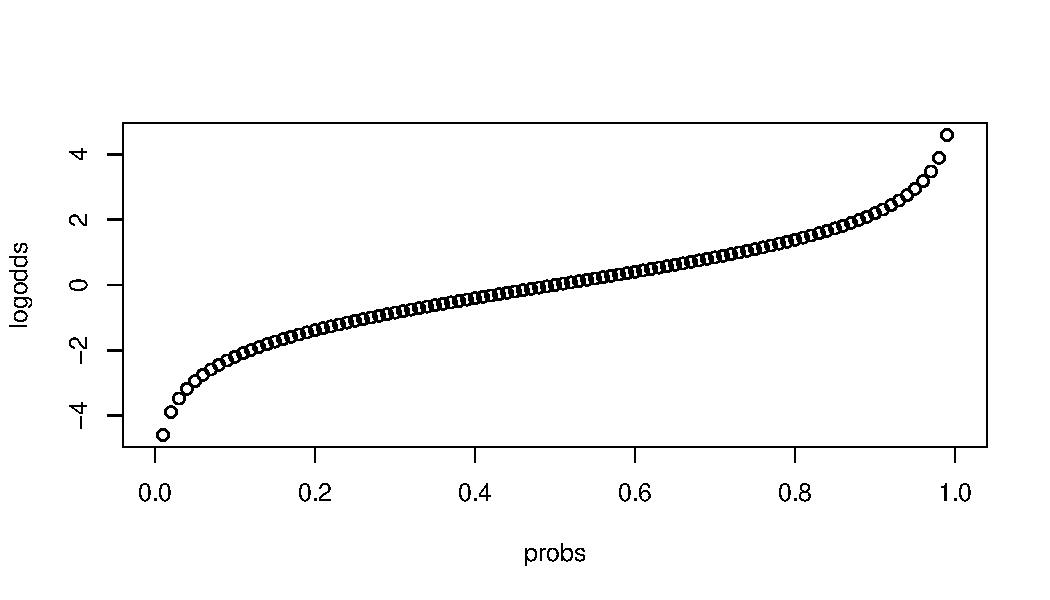
\includegraphics[width=\maxwidth]{figure/unnamed-chunk-73-1} 

\end{knitrout}
\caption{Impact of Dummy Variable}
\label{Fig:dummy}
\rule{4in}{1pt}
\end{figure}

\subsection{Non-Linear Regression}

We have really been sidestepping the fact that we really know how tree's trunk volume is related to its girth and height. Volume of a cylinder of radius $r$ and height $h$ is simply $\pi r^2 h$. So ideally we would want a regression model where $Girth$ and $Height$ are multiplied together - $y = \beta_0 x_1^{\beta_1} x_2^{\beta_2}$. This form of course does not meet the linearity assumption. However, we can transform the model into a linear one by taking log of both sides. This will give us the following model: $log y = Ln \beta_0 + \beta_1 log x_1 + \beta_2 log x_2$. Lets see how this looks in R.

\begin{knitrout}
\definecolor{shadecolor}{rgb}{0.969, 0.969, 0.969}\color{fgcolor}\begin{kframe}
\begin{alltt}
\hlstd{treeslog} \hlkwb{<-} \hlkwd{lm}\hlstd{(}\hlkwd{log}\hlstd{(Volume)} \hlopt{~} \hlkwd{log}\hlstd{(Girth)} \hlopt{+} \hlkwd{log}\hlstd{(Height),} \hlkwc{data} \hlstd{= trees)}
\hlkwd{summary}\hlstd{(treeslog)}
\end{alltt}
\begin{verbatim}
## 
## Call:
## lm(formula = log(Volume) ~ log(Girth) + log(Height), data = trees)
## 
## Residuals:
##       Min        1Q    Median        3Q       Max 
## -0.168561 -0.048488  0.002431  0.063637  0.129223 
## 
## Coefficients:
##             Estimate Std. Error t value Pr(>|t|)    
## (Intercept) -6.63162    0.79979  -8.292 5.06e-09 ***
## log(Girth)   1.98265    0.07501  26.432  < 2e-16 ***
## log(Height)  1.11712    0.20444   5.464 7.81e-06 ***
## ---
## Signif. codes:  0 '***' 0.001 '**' 0.01 '*' 0.05 '.' 0.1 ' ' 1
## 
## Residual standard error: 0.08139 on 28 degrees of freedom
## Multiple R-squared:  0.9777,	Adjusted R-squared:  0.9761 
## F-statistic: 613.2 on 2 and 28 DF,  p-value: < 2.2e-16
\end{verbatim}
\end{kframe}
\end{knitrout}

As we can see, this is our best model yet!

\section{Model Selection}

When we have several predictor variables available, the important question arises of which of those predictors to include in the regression model. Ideally, variable section should be done based on theoretical criteria and not analytical convenience. However, some times it may be necessary to choose variables to build the best model possible in absence of theoretical considerations. In this section we will look at stepwise regression using the command \texttt{step()}\index{R Commands!step}\marginpar{\small{\textbf{step}: stepwise method for variable selection}} as a method for selecting predictor variables. Then we will consider how to compare two different models using the function \texttt{anova()}\index{R Commands!anova}. \marginpar{\small{\textbf{anova}: used for comparing two models}}

The mathematical criterion for deciding whether to include or remove predictor variables is called \texttt{AIC}\index{Key Concepts!AIC} - Akaike Information Criterion - which is defined for a linear regression with $K$ predictor variables as: \( AIC = (SS_{res} / \sigma^2) + 2K \). For best model performance, we want the smallest AIC value. As number of predictors grow, without a corresponding significant decline in magnitude of residuals, the AIC goes up. Hence, minimizing AIC ensures that only predictors with significant impact on residuals are included in the model.

\subsection{Stepwise Regression}

We will explore our last model of trees' volume using Stepwise Regression (saved as model $treeslog$. The default stepwise mode is \texttt{backward elimination} where we start with a full model (all predictors included) and test removing a predictor variable in each step. The combination with lowest AIC is selected as the preferred model.  
\begin{knitrout}
\definecolor{shadecolor}{rgb}{0.969, 0.969, 0.969}\color{fgcolor}\begin{kframe}
\begin{alltt}
\hlkwd{step}\hlstd{(}\hlkwc{object} \hlstd{= treeslog,} \hlkwc{direction} \hlstd{=} \hlstr{"backward"}\hlstd{)}
\end{alltt}
\begin{verbatim}
## Start:  AIC=-152.69
## log(Volume) ~ log(Girth) + log(Height)
## 
##               Df Sum of Sq    RSS      AIC
## <none>                     0.1855 -152.685
## - log(Height)  1    0.1978 0.3832 -132.185
## - log(Girth)   1    4.6275 4.8130  -53.743
## 
## Call:
## lm(formula = log(Volume) ~ log(Girth) + log(Height), data = trees)
## 
## Coefficients:
## (Intercept)   log(Girth)  log(Height)  
##      -6.632        1.983        1.117
\end{verbatim}
\end{kframe}
\end{knitrout}

We can see in the output that when all predictors are included, the model has an AIC of $-152.69$. The output table shows that if any of the predictors are removed, the AIC value increases. Hence, we conclude that the full model is the best mode and we do not need to remove any predictors from our model.

We can also run the stepwise regression using \texttt{forward selection}. In this case we start with an empty model (only the intercept) and then additional predictors are added in each step until minimum AIC value is reached.

\begin{knitrout}
\definecolor{shadecolor}{rgb}{0.969, 0.969, 0.969}\color{fgcolor}\begin{kframe}
\begin{alltt}
\hlstd{emptymodel} \hlkwb{<-} \hlkwd{lm}\hlstd{(}\hlkwd{log}\hlstd{(Volume)} \hlopt{~} \hlnum{1}\hlstd{,} \hlkwc{data} \hlstd{= trees)}  \hlcom{#Start with an empty model}
\hlkwd{step}\hlstd{(}\hlkwc{object} \hlstd{= emptymodel,} \hlkwc{direction} \hlstd{=} \hlstr{"forward"}\hlstd{,} \hlkwc{scope} \hlstd{=} \hlkwd{log}\hlstd{(Volume)} \hlopt{~} \hlkwd{log}\hlstd{(Girth)} \hlopt{+}
    \hlkwd{log}\hlstd{(Height))}
\end{alltt}
\begin{verbatim}
## Start:  AIC=-38.82
## log(Volume) ~ 1
## 
##               Df Sum of Sq    RSS      AIC
## + log(Girth)   1    7.9254 0.3832 -132.185
## + log(Height)  1    3.4957 4.8130  -53.743
## <none>                     8.3087  -38.817
## 
## Step:  AIC=-132.19
## log(Volume) ~ log(Girth)
## 
##               Df Sum of Sq     RSS     AIC
## + log(Height)  1   0.19778 0.18546 -152.69
## <none>                     0.38324 -132.19
## 
## Step:  AIC=-152.69
## log(Volume) ~ log(Girth) + log(Height)
## 
## Call:
## lm(formula = log(Volume) ~ log(Girth) + log(Height), data = trees)
## 
## Coefficients:
## (Intercept)   log(Girth)  log(Height)  
##      -6.632        1.983        1.117
\end{verbatim}
\end{kframe}
\end{knitrout}

Output shows that the empty model (only an intercept) has an AIC of $-38.82$. In the first step one predictor is added and AIC reaches $-132.19$; then in the second step second predictor is added and AIC reaches the minimum value of $-152.69$. We reach the same optimal solution as in the backward elimination process before.

\subsection{Model Comparison}

We can directly compare two models as well. We will create a new model first for comparison purposes.

\begin{knitrout}
\definecolor{shadecolor}{rgb}{0.969, 0.969, 0.969}\color{fgcolor}\begin{kframe}
\begin{alltt}
\hlstd{trees}\hlopt{$}\hlstd{random} \hlkwb{<-} \hlkwd{rnorm}\hlstd{(}\hlkwd{nrow}\hlstd{(trees))}  \hlcom{#Random variable}
\hlstd{model.A} \hlkwb{<-} \hlkwd{lm}\hlstd{(}\hlkwd{log}\hlstd{(Volume)} \hlopt{~} \hlkwd{log}\hlstd{(Girth)} \hlopt{+} \hlkwd{log}\hlstd{(Height),} \hlkwc{data} \hlstd{= trees)}
\hlstd{model.B} \hlkwb{<-} \hlkwd{lm}\hlstd{(}\hlkwd{log}\hlstd{(Volume)} \hlopt{~} \hlkwd{log}\hlstd{(Girth)} \hlopt{+} \hlkwd{log}\hlstd{(Height)} \hlopt{+} \hlstd{trees}\hlopt{$}\hlstd{random,} \hlkwc{data} \hlstd{= trees)}
\end{alltt}
\end{kframe}
\end{knitrout}

Clearly model.B should not be better than model.A as the only difference is a random variable. However, how do we test the relative effectiveness of the two models. First, we can just calculate AIC values using the function \texttt{AIC()}\index{R Commands!AIC}. We can see in the output below that model.A has lower AIC values than model.B.

\begin{knitrout}
\definecolor{shadecolor}{rgb}{0.969, 0.969, 0.969}\color{fgcolor}\begin{kframe}
\begin{alltt}
\hlkwd{AIC}\hlstd{(model.A)}
\end{alltt}
\begin{verbatim}
## [1] -62.71125
\end{verbatim}
\begin{alltt}
\hlkwd{AIC}\hlstd{(model.B)}
\end{alltt}
\begin{verbatim}
## [1] -60.74817
\end{verbatim}
\end{kframe}
\end{knitrout}

We can also consider the subset model (model.A) as the null hypothesis, the superset model (model.B) as the alternate hypothesis and then use the function \texttt{anova()}\index{R Commands!anova} to check if we can reject the null hypothesis in the favor of the alternate hypothesis.

\begin{knitrout}
\definecolor{shadecolor}{rgb}{0.969, 0.969, 0.969}\color{fgcolor}\begin{kframe}
\begin{alltt}
\hlcom{# Null hypothesis first, then alternate hypothesis}
\hlkwd{anova}\hlstd{(model.A, model.B)}
\end{alltt}
\begin{verbatim}
## Analysis of Variance Table
## 
## Model 1: log(Volume) ~ log(Girth) + log(Height)
## Model 2: log(Volume) ~ log(Girth) + log(Height) + trees$random
##   Res.Df     RSS Df  Sum of Sq      F Pr(>F)
## 1     28 0.18546                            
## 2     27 0.18524  1 0.00022076 0.0322  0.859
\end{verbatim}
\end{kframe}
\end{knitrout}

As the output shows, with a p-value of higher than 0.05, we can not reject the null hypothesis. Thus the analysis shows that model.A is the preferred model.


\section{Conclusion and Word of Caution}

In this chapter, we introduced the idea of linear regression using OLS. We saw how to run linear regression model in R including extracting valuable information from the model. We then looked at various assumptions inherent in  OLS and how to test whether those assumptions hold in our model. Finally, we looked at model selection issues including stepwise regression and comparing different models.

\subsection{Linear Regression is NOT a Silver Bullet}

Linear regression is extremely popular. Modern statistical software has made building a linear regression model so easy that we are tempted to use it everywhere. Rarely do regression diagnostics - including testing of linear regression model assumptions, are carried out in a robust and reliable matter. Further, incorrect interpretation of regression model results is endemic. 

Linear regression is a specific tool valid only for specific contexts that meet its requirement. The regression analysis is going to be only as useful as the model it tries to estimate. Hence, utmost case must be taken in first designing a theoretically consistent model before the model is evaluated using regression analysis.

\chapterendsymbol





% !Rnw root = AABase.Rnw

\chapter{Generalized Linear Models}

\begin{flushright}

\textbf{\texttt{In God We Trust; All Others Must Bring Data}}

\emph{-- Willian Edwards Deming}

\end{flushright}

\vspace{12pt}


The Multiple Regression model we explored in the last chapter assumed that the error terms were independently and identically distributed as Normal. Generalized linear models ("GLM") extend the traditional multiple regression model to include error terms following different distributions. R provides the function \texttt{glm()}\index{R Commands!glm} to estimate generalized linear models in similar ways as the previously studied \texttt{lm()} function. The only additional information required by the \texttt{glm()} command is the $family$ argument that specifies the distribution of the error term.

We will begin our exploration of GLMs with most popular one - Logit Model or Logistic Regression for a binary response variable.

\section{Logistic Regression}

Logistic regression is used to model dichotomous outcome variables - variables that take binary values - True/False, Yes/No, 1/0 etc. Before we run a regression, the binary response variable needs to be transformed to a continuous variable of wide range. The standard approach is to calculate log odds - log of odds ratio. In the logit model the log odds of the outcome variable is modeled as the response to the linear combination of the predictor variables. Log-odds have the recognizable curve as shown in the Figure \ref{Fig:logodds}.

\begin{figure}
\centering
\rule{4in}{1pt}
\begin{knitrout}
\definecolor{shadecolor}{rgb}{0.969, 0.969, 0.969}\color{fgcolor}\begin{kframe}
\begin{alltt}
\hlstd{probs} \hlkwb{<-} \hlkwd{seq}\hlstd{(}\hlnum{0}\hlstd{,} \hlnum{1}\hlstd{,} \hlnum{0.01}\hlstd{)}
\hlstd{odds} \hlkwb{=} \hlstd{probs}\hlopt{/}\hlstd{(}\hlnum{1} \hlopt{-} \hlstd{probs)}
\hlstd{logodds} \hlkwb{=} \hlkwd{log}\hlstd{(odds)}
\hlkwd{plot}\hlstd{(logodds, probs)}
\end{alltt}
\end{kframe}
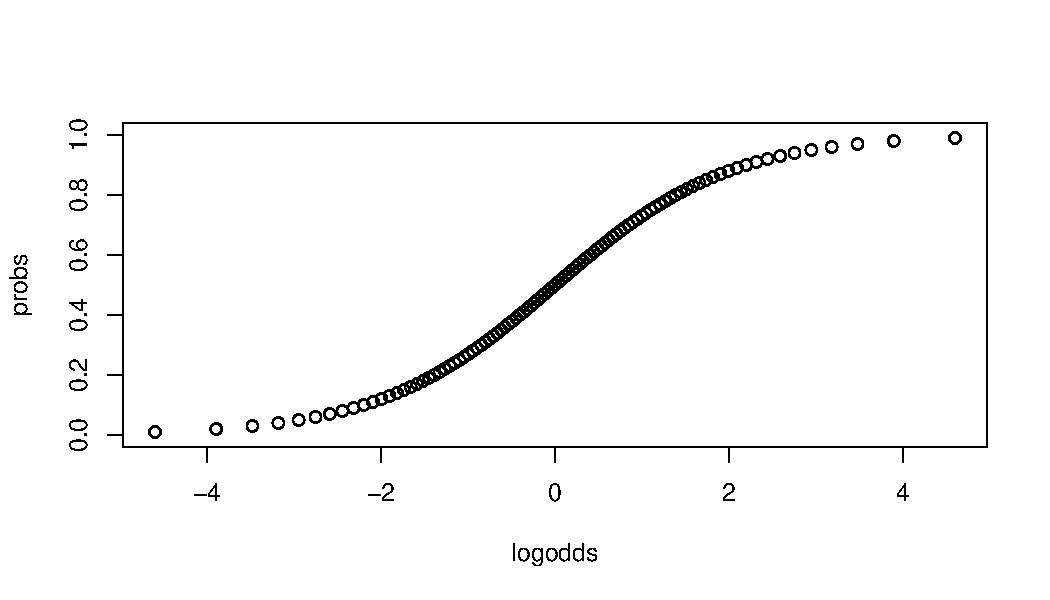
\includegraphics[width=\maxwidth]{figure/unnamed-chunk-80-1} 

\end{knitrout}
\caption{Plot of Log of Odds Ratio}
\label{Fig:logodds}
\rule{4in}{1pt}
\end{figure}

For illustrating logistic regression, we will use a dataset of 400 graduate school applications.
\begin{knitrout}
\definecolor{shadecolor}{rgb}{0.969, 0.969, 0.969}\color{fgcolor}\begin{kframe}
\begin{alltt}
\hlstd{admit.data} \hlkwb{<-} \hlkwd{read.csv}\hlstd{(}\hlstr{"binary.csv"}\hlstd{)}
\hlkwd{names}\hlstd{(admit.data)}
\end{alltt}
\begin{verbatim}
## [1] "admit" "gre"   "gpa"   "rank"
\end{verbatim}
\end{kframe}
\end{knitrout}

The dataset consists four columns - the outcome variable $admit$ is a binary variable. The predictor variables are $gre$ (the GRE score), $gpa$ (the undergrad GPA)  and $rank$ (a categorical variable from 1 to 4 indicating the status or prestige of the institution, with 1 denoting the highest prestige). 

We will first convert $rank$ as a factor and then run a logistic regression.
\begin{knitrout}
\definecolor{shadecolor}{rgb}{0.969, 0.969, 0.969}\color{fgcolor}\begin{kframe}
\begin{alltt}
\hlstd{admit.data}\hlopt{$}\hlstd{rank} \hlkwb{<-} \hlkwd{factor}\hlstd{(admit.data}\hlopt{$}\hlstd{rank)}
\hlstd{logit.model} \hlkwb{<-} \hlkwd{glm}\hlstd{(admit} \hlopt{~} \hlstd{gre} \hlopt{+} \hlstd{gpa} \hlopt{+} \hlstd{rank,} \hlkwc{data} \hlstd{= admit.data,} \hlkwc{family} \hlstd{=} \hlstr{"binomial"}\hlstd{)}
\hlkwd{summary}\hlstd{(logit.model)}
\end{alltt}
\begin{verbatim}
## 
## Call:
## glm(formula = admit ~ gre + gpa + rank, family = "binomial", 
##     data = admit.data)
## 
## Deviance Residuals: 
##     Min       1Q   Median       3Q      Max  
## -1.6268  -0.8662  -0.6388   1.1490   2.0790  
## 
## Coefficients:
##              Estimate Std. Error z value Pr(>|z|)    
## (Intercept) -3.989979   1.139951  -3.500 0.000465 ***
## gre          0.002264   0.001094   2.070 0.038465 *  
## gpa          0.804038   0.331819   2.423 0.015388 *  
## rank2       -0.675443   0.316490  -2.134 0.032829 *  
## rank3       -1.340204   0.345306  -3.881 0.000104 ***
## rank4       -1.551464   0.417832  -3.713 0.000205 ***
## ---
## Signif. codes:  0 '***' 0.001 '**' 0.01 '*' 0.05 '.' 0.1 ' ' 1
## 
## (Dispersion parameter for binomial family taken to be 1)
## 
##     Null deviance: 499.98  on 399  degrees of freedom
## Residual deviance: 458.52  on 394  degrees of freedom
## AIC: 470.52
## 
## Number of Fisher Scoring iterations: 4
\end{verbatim}
\end{kframe}
\end{knitrout}

While interpreting the output, keep in mind that the response variable modeled here is not the variable $admit$ but the log-odds of $admit$. The output of the model is similar to linear regression - we see residuals, coefficients and p-value - all with similar interpretations as before. We see that both $gre$ and $gpa$ are statistically significant (p-value < 0.05). The $rank$ factor has been converted into three dummy variables - all statistically significant. 

Looking at the coefficients, we can see that for 1 unit change in GRE score, log odds of admission increases by 0.002. Similarly, for 1 unit change in GPA, log odds of admission increases by 0.804. Attending an institution of rank 2 vs an institution of rank 1 reduces the log odds of admission by 0.6754.

Given a logistic regression model, we can conduct further significance tests using the \texttt{wald test} in the package \texttt{aod}. For example, we can test whether the $rank$ factors taken together are statistically significant or not. As the output below shows, the three factors taken together have a statistically significant impact. 
\begin{knitrout}
\definecolor{shadecolor}{rgb}{0.969, 0.969, 0.969}\color{fgcolor}\begin{kframe}
\begin{alltt}
\hlkwd{library}\hlstd{(aod)}
\hlkwd{wald.test}\hlstd{(}\hlkwc{b} \hlstd{=} \hlkwd{coef}\hlstd{(logit.model),} \hlkwc{Sigma} \hlstd{=} \hlkwd{vcov}\hlstd{(logit.model),} \hlkwc{Terms} \hlstd{=} \hlnum{4}\hlopt{:}\hlnum{6}\hlstd{)}
\end{alltt}
\begin{verbatim}
## Wald test:
## ----------
## 
## Chi-squared test:
## X2 = 20.9, df = 3, P(> X2) = 0.00011
\end{verbatim}
\end{kframe}
\end{knitrout}

Similarly, we can test whether it makes a difference whether the students comes from an institution of rank 3 of rank 4. While both these ranks had a statistically significant coefficients in the logit model, the magnitude of the coefficients show little difference - so its a relevant question to ask. As we can see from the output below, the effects of rank 3 and rank4 are in fact not statistically distinguishable as far as their impact on log odds of admission.
\begin{knitrout}
\definecolor{shadecolor}{rgb}{0.969, 0.969, 0.969}\color{fgcolor}\begin{kframe}
\begin{alltt}
\hlstd{coefflist} \hlkwb{<-} \hlkwd{cbind}\hlstd{(}\hlnum{0}\hlstd{,} \hlnum{0}\hlstd{,} \hlnum{0}\hlstd{,} \hlnum{0}\hlstd{,} \hlnum{1}\hlstd{,} \hlopt{-}\hlnum{1}\hlstd{)}
\hlkwd{wald.test}\hlstd{(}\hlkwc{b} \hlstd{=} \hlkwd{coef}\hlstd{(logit.model),} \hlkwc{Sigma} \hlstd{=} \hlkwd{vcov}\hlstd{(logit.model),} \hlkwc{L} \hlstd{= coefflist)}
\end{alltt}
\begin{verbatim}
## Wald test:
## ----------
## 
## Chi-squared test:
## X2 = 0.29, df = 1, P(> X2) = 0.59
\end{verbatim}
\end{kframe}
\end{knitrout}

As log odds are not intuitive to interpret, we can calculate coefficients as odds ratios. We can then use our model to predict probability of admission for a given set of input values.
\begin{knitrout}
\definecolor{shadecolor}{rgb}{0.969, 0.969, 0.969}\color{fgcolor}\begin{kframe}
\begin{alltt}
\hlkwd{exp}\hlstd{(}\hlkwd{coef}\hlstd{(logit.model))}
\end{alltt}
\begin{verbatim}
## (Intercept)         gre         gpa       rank2       rank3       rank4 
##   0.0185001   1.0022670   2.2345448   0.5089310   0.2617923   0.2119375
\end{verbatim}
\begin{alltt}
\hlstd{admitnew} \hlkwb{<-} \hlkwd{data.frame}\hlstd{(}\hlkwc{gre} \hlstd{=} \hlnum{700}\hlstd{,} \hlkwc{gpa} \hlstd{=} \hlnum{3.9}\hlstd{,} \hlkwc{rank} \hlstd{=} \hlnum{1}\hlstd{)}
\hlstd{admitnew}\hlopt{$}\hlstd{rank} \hlkwb{=} \hlkwd{factor}\hlstd{(admitnew}\hlopt{$}\hlstd{rank)}
\hlkwd{predict}\hlstd{(logit.model,} \hlkwc{newdata} \hlstd{= admitnew,} \hlkwc{type} \hlstd{=} \hlstr{"response"}\hlstd{)}
\end{alltt}
\begin{verbatim}
##         1 
## 0.6749952
\end{verbatim}
\end{kframe}
\end{knitrout}

Now we can say that a unit change in GPA improves the odds of being admitted by a factor of 2.23.

\section{Probit Model}

A probit model is also suitable for binary response variables.  In the probit model, the inverse standard normal distribution of the probability is modeled as a linear combination of the predictors. Probit transformation has a similar shape as logistic transformation as can be seen in Figure: \ref{Fig:probit}.

\begin{figure}
\centering
\rule{4in}{1pt}
\begin{knitrout}
\definecolor{shadecolor}{rgb}{0.969, 0.969, 0.969}\color{fgcolor}\begin{kframe}
\begin{alltt}
\hlkwd{library}\hlstd{(VGAM)}
\hlstd{probs} \hlkwb{<-} \hlkwd{seq}\hlstd{(}\hlnum{0}\hlstd{,} \hlnum{1}\hlstd{,} \hlnum{0.01}\hlstd{)}
\hlstd{probitdata} \hlkwb{<-} \hlkwd{probit}\hlstd{(probs)}
\hlkwd{plot}\hlstd{(probs, probitdata)}
\end{alltt}
\end{kframe}
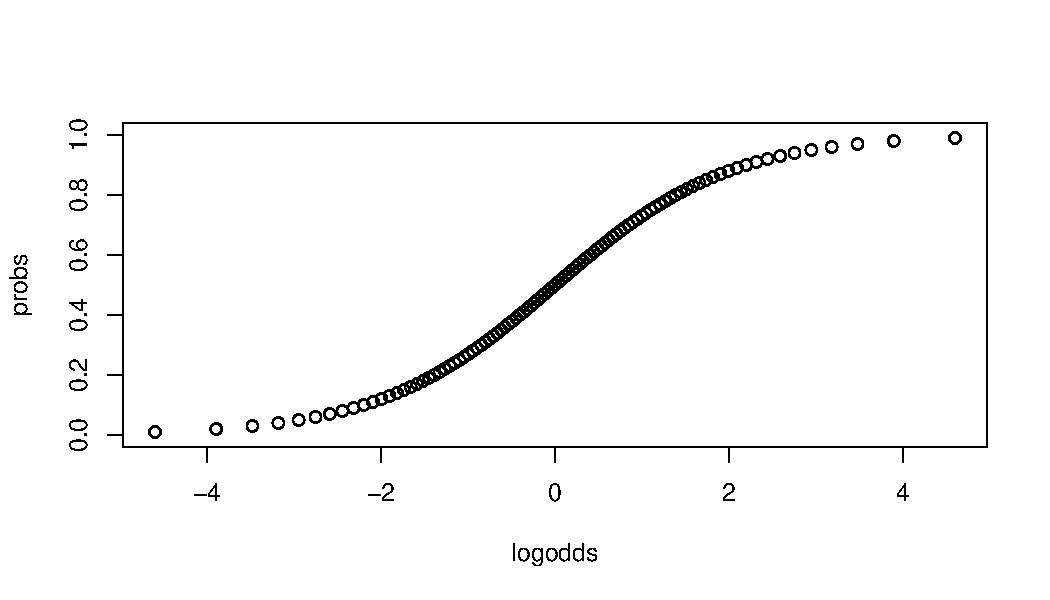
\includegraphics[width=\maxwidth]{figure/unnamed-chunk-86-1} 

\end{knitrout}
\caption{Plot of Probit Transformation}
\label{Fig:probit}
\rule{4in}{1pt}
\end{figure}

We can use the same \texttt{glm()} command to run a probit model. We need to specify $link$ as $probit$ to ensure that the model is run on a probit transformed outcome variable.
\begin{knitrout}
\definecolor{shadecolor}{rgb}{0.969, 0.969, 0.969}\color{fgcolor}\begin{kframe}
\begin{alltt}
\hlstd{probit.model} \hlkwb{<-} \hlkwd{glm}\hlstd{(admit} \hlopt{~} \hlstd{gre} \hlopt{+} \hlstd{gpa} \hlopt{+} \hlstd{rank,} \hlkwc{data} \hlstd{= admit.data,} \hlkwc{family} \hlstd{=} \hlkwd{binomial}\hlstd{(}\hlkwc{link} \hlstd{=} \hlstr{"probit"}\hlstd{))}
\hlkwd{summary}\hlstd{(probit.model)}
\end{alltt}
\begin{verbatim}
## 
## Call:
## glm(formula = admit ~ gre + gpa + rank, family = binomial(link = "probit"), 
##     data = admit.data)
## 
## Deviance Residuals: 
##     Min       1Q   Median       3Q      Max  
## -1.6163  -0.8710  -0.6389   1.1560   2.1035  
## 
## Coefficients:
##              Estimate Std. Error z value Pr(>|z|)    
## (Intercept) -2.386836   0.673946  -3.542 0.000398 ***
## gre          0.001376   0.000650   2.116 0.034329 *  
## gpa          0.477730   0.197197   2.423 0.015410 *  
## rank2       -0.415399   0.194977  -2.131 0.033130 *  
## rank3       -0.812138   0.208358  -3.898 9.71e-05 ***
## rank4       -0.935899   0.245272  -3.816 0.000136 ***
## ---
## Signif. codes:  0 '***' 0.001 '**' 0.01 '*' 0.05 '.' 0.1 ' ' 1
## 
## (Dispersion parameter for binomial family taken to be 1)
## 
##     Null deviance: 499.98  on 399  degrees of freedom
## Residual deviance: 458.41  on 394  degrees of freedom
## AIC: 470.41
## 
## Number of Fisher Scoring iterations: 4
\end{verbatim}
\end{kframe}
\end{knitrout}

Usually, logit and probit models are pretty much interchangeable. We can demonstrate the fact by calculating predicted probability for the same values as for logit before. As we can see from the output below, the predicted probabilities are nearly identical.
\begin{knitrout}
\definecolor{shadecolor}{rgb}{0.969, 0.969, 0.969}\color{fgcolor}\begin{kframe}
\begin{alltt}
\hlkwd{predict}\hlstd{(probit.model,} \hlkwc{newdata} \hlstd{= admitnew,} \hlkwc{type} \hlstd{=} \hlstr{"response"}\hlstd{)}
\end{alltt}
\begin{verbatim}
##         1 
## 0.6697505
\end{verbatim}
\end{kframe}
\end{knitrout}

Much of our discussion of logistic regression is also applicable to probit models as well. The actual logit and probit transformations show some difference only very close to the edges (near probability either 0 or 1). This leads to minor, non-significant differences in model fit.  However, logit models have the advantage of an easily interpretable result - log of odds ratio is easier to understand and interpret than the inverse of cumulative normal distribution. As a result, logistic regression is much more popular than probit regression.  

\section{Survival Analysis}

In last section we looked at modeling a binary response varioable. In this section, we extend out understanding to include the time taken for the event to happen. Essentially, we want to model the time duration for an event to occur. Examples of such models may include - time taken for a loan to default, time for a machine to fail, time until a stock market crash or time taken for seeds to getminate. Traditionally, survival models have been used to model time to death (hence the name survival). Survival analysis is often called Duration Analysis or Failure Time Analysis as well.

We did not go into much theoretical details for Linear Regression and Logistic Regression as it was assumed that students have had prior exposure to those models (in the course pre-req TO301). As survival analysis is likely to be a new concept for most students, this writeup provides a deeper theoretical exploration than we did for previous topics.

\subsection{Survival Data}

Our main focus in survival analysis is survival time or "time to event". While time to event is a continuous variable, it is difficult to model it using linear regression because of non-normality and censoring. Non-normality occurs from the fact that time to event typically follows exponential distribution. The non-normality aspect of the data violates the normality assumption of OLS linear regression.  Time to event data is also typically right-censored - meaning that the information may be incomplete as the some observations do not get enough time to fail during the period under study. The most common context of survival analysis includes following subjects over time and observe at which point in time they experience the event of interest. It is typical that the study is not long enough to allow the event to occur for all the subjects in the study; resulting in a right censored data. Subjects also drop out of studies for various reasons leading to further right censoring. We use the name right censored because in this case the missing observations are further to the right end of the x-axis (if we plot time on x-axis).

Our main purpose in doing survival analysis is to examine relationships between survival time and one or more predictors (usually called covariates in survival models). The most widely used modeling technique for the purpose is the Cox Proportional Hazard Regression Model. This will the focus of our discussion. 

\subsection{Hazard Rate}

We are primarily interested in the Survival Functiion $S(t) = Prob(T > t) = 1 - P(t)$ where $T$ is the survival time and $P(t)$ is the Cumulative Probability Density Function of $T$. We typically assume that $S(0) = 1$, $S(t) = 0$ as $t \rightarrow \infty $ and ${d S(t)}/{dt} <= 0$. 

Key to survival analysis is the concept of hazard rate - also called hazard function. Hazard rate can be defined as the probability that an event will occur at time \texttt{t} assuming that the event has not already happened by then. Another way to think about it is to suppose that a subject has survived until time $t$ and then calculate the probability that it will not survive for an additional time $dt$ with $dt \rightarrow \infty$. Essentially, hazard rate at time $t$, often denoted as $h(t)$ is the rate at which events occur at time $t$. Hazard rate (most commonly log of hazard rate) is typically used as the response variable in survival analysis. 

Mathematically, we can calculate that $h(t) = f(t) / S(t)$ where $f(t)$ is the probability density function of $T$ and $S(t)$, as we saw above, is the survival function. A constant hazard rate, $h(t) = k$ implies an exponential distribution of survival times with probability density function $p(t) = k e^{-kt}$. 

Other common hazard function specifications include: $log(h(t)) = k + \rho t $ leading to Gompertz distribution of survival time, and $log(h(t)) = k + \rho log(t)$ leading to Weibull distribution of survival time. While several parametric regresison models exist for estimating specific functional form of hazard rate, we will focus on the \texttt{Cox Model}\index{Key Concepts!Cox Model} that leaves the baseline hazard function unspecified as the general form $log(h_0(t)) = \alpha(t)$. Including covariates $x_1$ through $x_n$, our model to be estimated becomes:

$$log(h(t)) = \alpha(t) + \beta_1 x_1 + \beta_2 x_2 + ... + \beta_n x_n$$ or equivalently,

$$h(t) = e^{\alpha(t)} e^{(\beta_1 x_1 + \beta_2 x_2 + ... + \beta_n x_n)}$$ which reduces to $$h(t) = e^{\alpha(t)} e^{\eta}$$ where $$\eta = (\beta_1 x_1 + \beta_2 x_2 + ... + \beta_n x_n)$$ is the linear predictor. We can see that if we have two observations $i$ and $j$ then the hazard ratio for these two observations $$\frac{h_i(t)}{h_j(t)} = \frac{e ^ {\eta_{i}}}{e ^ {\eta_{j}}}$$ is independent of time $t$. As the hazard rate is proportional to the the linear predictor, this model is also known as the \textbf{Cox Proportional Hazards Model}.  

\subsection{Survival Analysis in R}

We will use the \texttt{OIsurv}\index{Packages!OIsurv}\index{Packages!survival}\index{Packages!KMsurv} packages which loads the other two required packages \texttt{survival} (which has the required functions) and \texttt{KMsurv} (which has some useful datasets for survival analysis)


\begin{knitrout}
\definecolor{shadecolor}{rgb}{0.969, 0.969, 0.969}\color{fgcolor}\begin{kframe}
\begin{alltt}
\hlcom{# install.packages\{'OIsurv\} #Output suppressed for brevity}
\hlkwd{library}\hlstd{(OIsurv)}
\hlkwd{library}\hlstd{(survival)}
\end{alltt}
\end{kframe}
\end{knitrout}

Most functions in the $survival$ package need survival objects created by the \texttt{Surv()}\index{R Commands!Surv} function. For right censored data, survival objects can be created using two arguments to the $Surv$ function - the event time or the censoring time and a dummy variable coded 1 if the event occured or 0 of the observation is censored.  

We will use a dataset on Recidivism to illustrate the process of survival analysis in R. The dataset contains observations for a year of make prisoners after being released from prison. The dataset has the following variables:
\begin{itemize}
\item \texttt{week}: Number of weeks to get arrested again, or censoring time in case the subject does not get arrested during study period
\item \texttt{arrest}: dummy variable to indicate whether the subject was arrested during the study period; 1: Yes, 0: No.
\item \texttt{fin}: Whether the subject received financial assistance; 1: Yes, 0: No.
\item \texttt{age}: in years at the time of release from prison.
\item \texttt{race}: 1 for African American, 0 for all others
\item \texttt{wexp}: Full time work experience before incarneation; 1: Yes, 0: No
\item \texttt{mar}: Whether the subject was married at the time of release; 1: Yes, 0: No.
\item \texttt{paro}: Whether the subject was released on parole;  1: Yes, 0: No.
\item \texttt{prio}: Number of prior convictions.
\item \texttt{educ}: Education level; 2: grade 6 or less, 3: grades 6 through 9, 4: grades 10 and 11, 5: grade 12, or 6: some post-secondary.
\item \texttt{emp1 - emp52}: Dummy variables; 1 if the subject was employed in the corresponding week of the study; 0 otherwise.
\end{itemize}

We will start by importing the data and taking a quick look inside.
\begin{knitrout}
\definecolor{shadecolor}{rgb}{0.969, 0.969, 0.969}\color{fgcolor}\begin{kframe}
\begin{alltt}
\hlstd{rossi} \hlkwb{<-} \hlkwd{read.table}\hlstd{(}\hlstr{"Rossi.txt"}\hlstd{,} \hlkwc{header} \hlstd{=} \hlnum{TRUE}\hlstd{)}
\hlstd{rossi[}\hlnum{1}\hlopt{:}\hlnum{5}\hlstd{,} \hlnum{1}\hlopt{:}\hlnum{15}\hlstd{]}  \hlcom{#First five rows, first 15 columns}
\end{alltt}
\begin{verbatim}
##   week arrest fin age race wexp mar paro prio educ emp1 emp2 emp3 emp4
## 1   20      1   0  27    1    0   0    1    3    3    0    0    0    0
## 2   17      1   0  18    1    0   0    1    8    4    0    0    0    0
## 3   25      1   0  19    0    1   0    1   13    3    0    0    0    0
## 4   52      0   1  23    1    1   1    1    1    5    0    0    0    0
## 5   52      0   0  19    0    1   0    1    3    3    0    0    0    0
##   emp5
## 1    0
## 2    0
## 3    0
## 4    1
## 5    0
\end{verbatim}
\end{kframe}
\end{knitrout}

First two columns are most important here. First column is the time stamp of observation in number of weeks; second column is whether the subject was rearrested (\texttt{arrest} = 1) or not (\texttt{arrest} = 0) at that time. So the first subject was rearrested in week 20th. A \texttt{week} = 52 and \texttt{arrest} = 0 (like the fourth row) means that the subject was never arrested until the study ended with the censoring time of 52.

Lets take a look at the structure of the data and make needed changes.
\begin{knitrout}
\definecolor{shadecolor}{rgb}{0.969, 0.969, 0.969}\color{fgcolor}\begin{kframe}
\begin{alltt}
\hlkwd{str}\hlstd{(rossi[,} \hlnum{1}\hlopt{:}\hlnum{10}\hlstd{])}
\end{alltt}
\begin{verbatim}
## 'data.frame':	432 obs. of  10 variables:
##  $ week  : int  20 17 25 52 52 52 23 52 52 52 ...
##  $ arrest: int  1 1 1 0 0 0 1 0 0 0 ...
##  $ fin   : int  0 0 0 1 0 0 0 1 0 0 ...
##  $ age   : int  27 18 19 23 19 24 25 21 22 20 ...
##  $ race  : int  1 1 0 1 0 1 1 1 1 1 ...
##  $ wexp  : int  0 0 1 1 1 1 1 1 0 1 ...
##  $ mar   : int  0 0 0 1 0 0 1 0 0 0 ...
##  $ paro  : int  1 1 1 1 1 0 1 1 0 0 ...
##  $ prio  : int  3 8 13 1 3 2 0 4 6 0 ...
##  $ educ  : int  3 4 3 5 3 4 4 3 3 5 ...
\end{verbatim}
\end{kframe}
\end{knitrout}

Seems like several factors are coded as numbers. In contrast to how we approached them before, we will leave them as numbers (its a good exercise to change them to factors and see what breaks in following pages). We first build the survival object.
\begin{knitrout}
\definecolor{shadecolor}{rgb}{0.969, 0.969, 0.969}\color{fgcolor}\begin{kframe}
\begin{alltt}
\hlstd{rossi.surv} \hlkwb{<-} \hlkwd{Surv}\hlstd{(rossi}\hlopt{$}\hlstd{week, rossi}\hlopt{$}\hlstd{arrest)}
\end{alltt}
\end{kframe}
\end{knitrout}

We can now use this survival object as the response variable in a Cox model. Cox models can be run using the \texttt{coxph()}\index{R Commands!coxph} in the $survival$ package. We will start by using all the variables except $emp1 - emp52$ dummy variables. The syntax of $coxph()$ is quite similar to the $lm()$ and $glm()$ syntax we have already seen.
\begin{knitrout}
\definecolor{shadecolor}{rgb}{0.969, 0.969, 0.969}\color{fgcolor}\begin{kframe}
\begin{alltt}
\hlstd{mod.first} \hlkwb{<-} \hlkwd{coxph}\hlstd{(rossi.surv} \hlopt{~} \hlstd{fin} \hlopt{+} \hlstd{age} \hlopt{+} \hlstd{race} \hlopt{+} \hlstd{wexp} \hlopt{+} \hlstd{mar} \hlopt{+} \hlstd{paro} \hlopt{+} \hlstd{prio} \hlopt{+}
    \hlstd{educ,} \hlkwc{data} \hlstd{= rossi)}
\hlkwd{summary}\hlstd{(mod.first)}
\end{alltt}
\begin{verbatim}
## Call:
## coxph(formula = rossi.surv ~ fin + age + race + wexp + mar + 
##     paro + prio + educ, data = rossi)
## 
##   n= 432, number of events= 114 
## 
##          coef exp(coef) se(coef)      z Pr(>|z|)   
## fin  -0.35963   0.69794  0.19180 -1.875  0.06079 . 
## age  -0.05768   0.94395  0.02187 -2.638  0.00835 **
## race  0.34554   1.41276  0.30907  1.118  0.26356   
## wexp -0.11439   0.89191  0.21311 -0.537  0.59145   
## mar  -0.42496   0.65380  0.38209 -1.112  0.26605   
## paro -0.08991   0.91401  0.19568 -0.459  0.64589   
## prio  0.08469   1.08838  0.02919  2.902  0.00371 **
## educ -0.18578   0.83046  0.13153 -1.412  0.15782   
## ---
## Signif. codes:  0 '***' 0.001 '**' 0.01 '*' 0.05 '.' 0.1 ' ' 1
## 
##      exp(coef) exp(-coef) lower .95 upper .95
## fin     0.6979     1.4328    0.4792    1.0164
## age     0.9440     1.0594    0.9044    0.9853
## race    1.4128     0.7078    0.7709    2.5891
## wexp    0.8919     1.1212    0.5874    1.3543
## mar     0.6538     1.5295    0.3092    1.3825
## paro    0.9140     1.0941    0.6229    1.3413
## prio    1.0884     0.9188    1.0279    1.1525
## educ    0.8305     1.2042    0.6417    1.0747
## 
## Concordance= 0.656  (se = 0.027 )
## Rsquare= 0.079   (max possible= 0.956 )
## Likelihood ratio test= 35.35  on 8 df,   p=2.31e-05
## Wald test            = 33.74  on 8 df,   p=4.529e-05
## Score (logrank) test = 35.1  on 8 df,   p=2.568e-05
\end{verbatim}
\end{kframe}
\end{knitrout}

Interpretation of the results is very similar to interpretation of linear regression output. The coefficients show the impact of unit change in predictor variable on the response variable (in this case log hazard ratio). Statistical significance can be checked with the p-value in the last column. So, we can say that the log hazard rate for subjects who were provided financial aid $(fin = 1)$ is 0.40 less than log hazard rate for subjects who were not provided financial aid $(fin = 0)$; and the effect is statistically significant. Predictors $age$ and $prio$ (prior convictions) were also found to be statistically significant. 

As interpreting log hazard rates can be cumbersome, the output also provides exponentiated coefficients - which can be interpreted as multiplicative effects on the hazard rate. For example, $age$ has a coefficient $\beta = -0.05$ and exponentiated coefficient $e^\beta = 0.95$. That means that with increase of 1 in $age$, the hazard rate is 0.95 times the original value - a reduction of 5\%. Similarly, we can see that an increase of one in prior convictions leads to an increase in log hazard rate of 0.079 and the hazard rate is multiplied by a factor of 1.08 (i.e. an increase of 8\% in hazard rate).

Model significance is shown by the Likelihood Ratio Test, Wald Test and Score Test which tests the null hypothesis that all the coefficients are zero. As the results show, the null hypothesis is rejected and the model is found significant. The R-Square value can be interpreted in a similar manner as in linear regression.

Now that we have a suitable model, we can now examine the estimated distribution of survival times using the \texttt{survfit()}\index{R Commands!survfit} function that estimates the survival function $S(t)$ at the mean values of all predictors. Figure \ref{Fig:survfit} shows the survival function for our analysis including the 95\% confidence band.
\begin{figure}
\centering
\rule{4in}{1pt}
\begin{knitrout}
\definecolor{shadecolor}{rgb}{0.969, 0.969, 0.969}\color{fgcolor}\begin{kframe}
\begin{alltt}
\hlkwd{plot}\hlstd{(}\hlkwd{survfit}\hlstd{(mod.first),} \hlkwc{ylim} \hlstd{=} \hlkwd{c}\hlstd{(}\hlnum{0.75}\hlstd{,} \hlnum{1}\hlstd{),} \hlkwc{xlab} \hlstd{=} \hlstr{"Weeks of Observation"}\hlstd{,} \hlkwc{ylab} \hlstd{=} \hlstr{"Proportion of Subject Not Rearrested"}\hlstd{)}
\end{alltt}
\end{kframe}
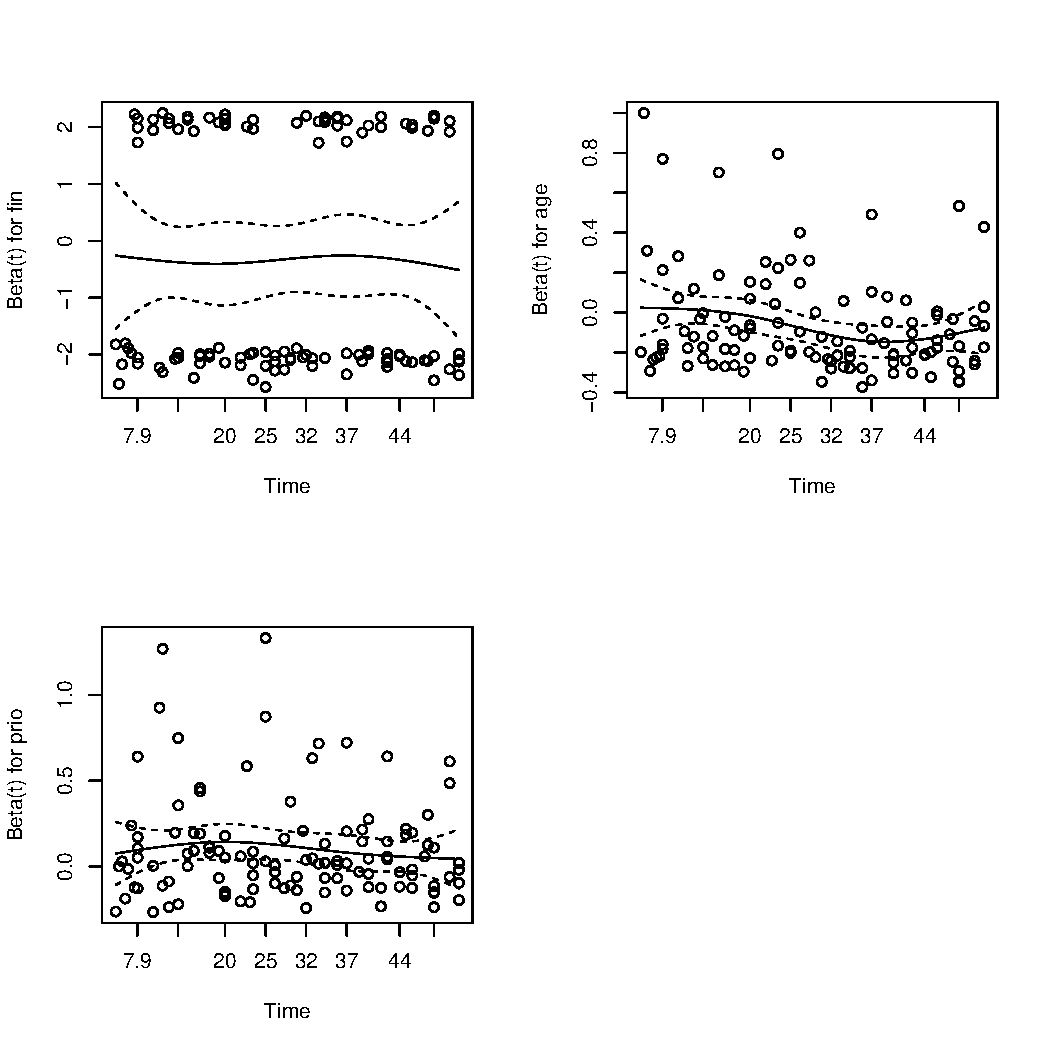
\includegraphics[width=\maxwidth]{figure/unnamed-chunk-95-1} 

\end{knitrout}
\caption{Plot of Survival Function}
\label{Fig:survfit}
\rule{4in}{1pt}
\end{figure}

\subsection{Time Dependent Covariates}

The previous model assumed that the effect of covariates on the survival object was independent of the the time parameter. The $coxph$ function allows for time dependent covariates as well. However, in such cases it requires that data for each time period for a subject appear as a separate record (or row) in the data set. For example - we have 52 weeks of employment data in our dataset - but each week is coded as a column. To include employment data (which is time dependent) we will need to first reshape the data in what is commonly known as the "long form".

\begin{knitrout}
\definecolor{shadecolor}{rgb}{0.969, 0.969, 0.969}\color{fgcolor}\begin{kframe}
\begin{alltt}
\hlcom{## Change to the long format}
\hlstd{rossi.long} \hlkwb{<-} \hlkwd{reshape}\hlstd{(}\hlkwc{data} \hlstd{= rossi,} \hlkwc{varying} \hlstd{=} \hlkwd{paste0}\hlstd{(}\hlstr{"emp"}\hlstd{,} \hlnum{1}\hlopt{:}\hlnum{52}\hlstd{),} \hlkwc{v.names} \hlstd{=} \hlstr{"employed"}\hlstd{,}
    \hlkwc{timevar} \hlstd{=} \hlstr{"time"}\hlstd{,} \hlkwc{idvar} \hlstd{=} \hlstr{"id"}\hlstd{,} \hlkwc{direction} \hlstd{=} \hlstr{"long"}\hlstd{,} \hlkwc{sep} \hlstd{=} \hlstr{""}\hlstd{)}

\hlcom{## Sort by id and time}
\hlkwd{library}\hlstd{(doBy)}
\hlstd{rossi.long} \hlkwb{<-} \hlkwd{orderBy}\hlstd{(}\hlopt{~+}\hlstd{id} \hlopt{+} \hlstd{time,} \hlkwc{data} \hlstd{= rossi.long)}

\hlcom{## Drop rows where emp is NA (time after event/censoring)}
\hlstd{rossi.long} \hlkwb{<-} \hlstd{rossi.long[}\hlopt{!}\hlkwd{is.na}\hlstd{(rossi.long}\hlopt{$}\hlstd{emp), ]}
\hlkwd{head}\hlstd{(rossi.long)}
\end{alltt}
\begin{verbatim}
##     week arrest fin age race wexp mar paro prio educ time employed id
## 1.1   20      1   0  27    1    0   0    1    3    3    1        0  1
## 1.2   20      1   0  27    1    0   0    1    3    3    2        0  1
## 1.3   20      1   0  27    1    0   0    1    3    3    3        0  1
## 1.4   20      1   0  27    1    0   0    1    3    3    4        0  1
## 1.5   20      1   0  27    1    0   0    1    3    3    5        0  1
## 1.6   20      1   0  27    1    0   0    1    3    3    6        0  1
\end{verbatim}
\end{kframe}
\end{knitrout}

For time varing covariates, we will need start and stop time for each time interval and the corresponding value of the time varying covariates for that time interval. We want to check for two such covariates: whether employed during current time period or whether employed during last (lagged by 1) time period. The following code calculated the values in the long form.
\begin{knitrout}
\definecolor{shadecolor}{rgb}{0.969, 0.969, 0.969}\color{fgcolor}\begin{kframe}
\begin{alltt}
\hlkwd{library}\hlstd{(plyr)}  \hlcom{# Load plyr package}

\hlcom{# Create time variables and various forms of exposure variables}
\hlstd{rossi.long} \hlkwb{<-} \hlkwd{ddply}\hlstd{(}\hlkwc{.data} \hlstd{= rossi.long,} \hlkwc{.variables} \hlstd{=} \hlkwd{c}\hlstd{(}\hlstr{"id"}\hlstd{),} \hlkwc{.drop} \hlstd{=} \hlnum{TRUE}\hlstd{,}
    \hlkwc{.fun} \hlstd{=} \hlkwa{function}\hlstd{(}\hlkwc{DF}\hlstd{) \{}
        \hlstd{DF}\hlopt{$}\hlstd{start} \hlkwb{<-} \hlkwd{c}\hlstd{(}\hlnum{0}\hlstd{,} \hlkwd{head}\hlstd{(DF}\hlopt{$}\hlstd{time,} \hlopt{-}\hlnum{1}\hlstd{))}  \hlcom{# Start of each interval}
        \hlstd{DF}\hlopt{$}\hlstd{stop} \hlkwb{<-} \hlstd{DF}\hlopt{$}\hlstd{time}  \hlcom{# End of each interval}
        \hlstd{DF}\hlopt{$}\hlstd{event} \hlkwb{<-} \hlnum{0}  \hlcom{# Event indicator for each interval}
        \hlstd{DF[}\hlkwd{nrow}\hlstd{(DF),} \hlstr{"event"}\hlstd{]} \hlkwb{<-} \hlstd{DF[}\hlkwd{nrow}\hlstd{(DF),} \hlstr{"arrest"}\hlstd{]}  \hlcom{# Arrest value }
        \hlstd{DF}\hlopt{$}\hlstd{employed.lag1} \hlkwb{<-} \hlkwd{c}\hlstd{(}\hlkwd{rep}\hlstd{(}\hlnum{NA}\hlstd{,} \hlnum{1}\hlstd{),} \hlkwd{head}\hlstd{(DF}\hlopt{$}\hlstd{employed,} \hlopt{-}\hlnum{1}\hlstd{))}
        \hlstd{DF}  \hlcom{# Return DF }
    \hlstd{\})}
\hlstd{rossi.long[rossi.long}\hlopt{$}\hlstd{id} \hlopt{==} \hlnum{2}\hlstd{,} \hlkwd{c}\hlstd{(}\hlstr{"id"}\hlstd{,} \hlstr{"start"}\hlstd{,} \hlstr{"stop"}\hlstd{,} \hlstr{"event"}\hlstd{,} \hlstr{"employed"}\hlstd{,}
    \hlstr{"employed.lag1"}\hlstd{)]}
\end{alltt}
\begin{verbatim}
##    id start stop event employed employed.lag1
## 21  2     0    1     0        0            NA
## 22  2     1    2     0        0             0
## 23  2     2    3     0        0             0
## 24  2     3    4     0        0             0
## 25  2     4    5     0        0             0
## 26  2     5    6     0        0             0
## 27  2     6    7     0        0             0
## 28  2     7    8     0        0             0
## 29  2     8    9     0        0             0
## 30  2     9   10     0        1             0
## 31  2    10   11     0        1             1
## 32  2    11   12     0        1             1
## 33  2    12   13     0        1             1
## 34  2    13   14     0        1             1
## 35  2    14   15     0        0             1
## 36  2    15   16     0        0             0
## 37  2    16   17     1        0             0
\end{verbatim}
\end{kframe}
\end{knitrout}

\index{Packages!plyr}The data for subject id = 2 shows the time dependent covariates in the long form. We can see that the subject was rearrested in the 17th week. We can also see that the subject was employed from 10th to 14th week. 

We are now ready to run a cox model with time dependent covariates. We start by checking whether being employed in a week affects the chances of a subject getting arrested in that week.

\begin{knitrout}
\definecolor{shadecolor}{rgb}{0.969, 0.969, 0.969}\color{fgcolor}\begin{kframe}
\begin{alltt}
\hlstd{mod.timed} \hlkwb{<-} \hlkwd{coxph}\hlstd{(}\hlkwd{Surv}\hlstd{(start, stop, event)} \hlopt{~} \hlstd{fin} \hlopt{+} \hlstd{age} \hlopt{+} \hlstd{race} \hlopt{+} \hlstd{wexp} \hlopt{+} \hlstd{mar} \hlopt{+}
    \hlstd{paro} \hlopt{+} \hlstd{prio} \hlopt{+} \hlstd{employed,} \hlkwc{data} \hlstd{= rossi.long)}
\hlkwd{summary}\hlstd{(mod.timed)}
\end{alltt}
\begin{verbatim}
## Call:
## coxph(formula = Surv(start, stop, event) ~ fin + age + race + 
##     wexp + mar + paro + prio + employed, data = rossi.long)
## 
##   n= 19809, number of events= 114 
## 
##              coef exp(coef) se(coef)      z Pr(>|z|)    
## fin      -0.35672   0.69997  0.19113 -1.866  0.06198 .  
## age      -0.04634   0.95472  0.02174 -2.132  0.03301 *  
## race      0.33866   1.40306  0.30960  1.094  0.27402    
## wexp     -0.02555   0.97477  0.21142 -0.121  0.90380    
## mar      -0.29375   0.74546  0.38303 -0.767  0.44314    
## paro     -0.06421   0.93781  0.19468 -0.330  0.74156    
## prio      0.08514   1.08887  0.02896  2.940  0.00328 ** 
## employed -1.32832   0.26492  0.25072 -5.298 1.17e-07 ***
## ---
## Signif. codes:  0 '***' 0.001 '**' 0.01 '*' 0.05 '.' 0.1 ' ' 1
## 
##          exp(coef) exp(-coef) lower .95 upper .95
## fin         0.7000     1.4286    0.4813    1.0180
## age         0.9547     1.0474    0.9149    0.9963
## race        1.4031     0.7127    0.7648    2.5740
## wexp        0.9748     1.0259    0.6441    1.4753
## mar         0.7455     1.3414    0.3519    1.5793
## paro        0.9378     1.0663    0.6403    1.3735
## prio        1.0889     0.9184    1.0288    1.1525
## employed    0.2649     3.7747    0.1621    0.4330
## 
## Concordance= 0.708  (se = 0.027 )
## Rsquare= 0.003   (max possible= 0.066 )
## Likelihood ratio test= 68.65  on 8 df,   p=9.114e-12
## Wald test            = 56.15  on 8 df,   p=2.632e-09
## Score (logrank) test = 64.48  on 8 df,   p=6.102e-11
\end{verbatim}
\end{kframe}
\end{knitrout}

The result show that the time dependent covariate - $employed$ has a large effect on the hazaes of rearrest. The hazard rate for a time period is smaller by a factor of 0.2649 (i.e. 73.5\% less) when the subject is employed during the  said time period. This large effect is a bit misleading though as it may be a result of reverse causality - the subject can't work if he has been arrested. So a better model would be to check whether being employed in the previous time period has an impact on the hazard rate of getting rearrested in the next time period.

\begin{knitrout}
\definecolor{shadecolor}{rgb}{0.969, 0.969, 0.969}\color{fgcolor}\begin{kframe}
\begin{alltt}
\hlstd{mod.lagtimed} \hlkwb{<-} \hlkwd{coxph}\hlstd{(}\hlkwd{Surv}\hlstd{(start, stop, event)} \hlopt{~} \hlstd{fin} \hlopt{+} \hlstd{age} \hlopt{+} \hlstd{race} \hlopt{+} \hlstd{wexp} \hlopt{+} \hlstd{mar} \hlopt{+}
    \hlstd{paro} \hlopt{+} \hlstd{prio} \hlopt{+} \hlstd{employed.lag1,} \hlkwc{data} \hlstd{= rossi.long)}
\hlkwd{summary}\hlstd{(mod.lagtimed)}
\end{alltt}
\begin{verbatim}
## Call:
## coxph(formula = Surv(start, stop, event) ~ fin + age + race + 
##     wexp + mar + paro + prio + employed.lag1, data = rossi.long)
## 
##   n= 19377, number of events= 113 
##    (432 observations deleted due to missingness)
## 
##                   coef exp(coef) se(coef)      z Pr(>|z|)    
## fin           -0.35130   0.70377  0.19181 -1.831 0.067035 .  
## age           -0.04977   0.95144  0.02189 -2.274 0.022969 *  
## race           0.32147   1.37915  0.30912  1.040 0.298369    
## wexp          -0.04764   0.95348  0.21323 -0.223 0.823207    
## mar           -0.34476   0.70839  0.38322 -0.900 0.368310    
## paro          -0.04710   0.95399  0.19630 -0.240 0.810375    
## prio           0.09199   1.09635  0.02880  3.194 0.001402 ** 
## employed.lag1 -0.78689   0.45526  0.21808 -3.608 0.000308 ***
## ---
## Signif. codes:  0 '***' 0.001 '**' 0.01 '*' 0.05 '.' 0.1 ' ' 1
## 
##               exp(coef) exp(-coef) lower .95 upper .95
## fin              0.7038     1.4209    0.4832    1.0250
## age              0.9514     1.0510    0.9115    0.9932
## race             1.3792     0.7251    0.7525    2.5278
## wexp             0.9535     1.0488    0.6278    1.4481
## mar              0.7084     1.4116    0.3343    1.5013
## paro             0.9540     1.0482    0.6493    1.4016
## prio             1.0964     0.9121    1.0362    1.1600
## employed.lag1    0.4553     2.1966    0.2969    0.6981
## 
## Concordance= 0.67  (se = 0.027 )
## Rsquare= 0.002   (max possible= 0.067 )
## Likelihood ratio test= 47.16  on 8 df,   p=1.43e-07
## Wald test            = 43.37  on 8 df,   p=7.483e-07
## Score (logrank) test = 46.4  on 8 df,   p=1.993e-07
\end{verbatim}
\end{kframe}
\end{knitrout}

As the results above show, being employed in the previous week reduces the hazard rate of being rearrested by a factor of 0.455 (i.e. a reduction of 54.5\%). A large and statistically significant result (p-value < 0.05).

\subsection{Model Diagnostics for Cox Regression}

Just like for linear regression, it is essential that we check that the data fits the basic assumptions inherent in running a Cox regression model. We will do model disgnostics on a smaller model with only the significant coefficients.
\begin{knitrout}
\definecolor{shadecolor}{rgb}{0.969, 0.969, 0.969}\color{fgcolor}\begin{kframe}
\begin{alltt}
\hlstd{mod.small} \hlkwb{<-} \hlkwd{coxph}\hlstd{(}\hlkwd{Surv}\hlstd{(week, arrest)} \hlopt{~} \hlstd{fin} \hlopt{+} \hlstd{age} \hlopt{+} \hlstd{prio,} \hlkwc{data} \hlstd{= rossi)}
\hlstd{mod.small}
\end{alltt}
\begin{verbatim}
## Call:
## coxph(formula = Surv(week, arrest) ~ fin + age + prio, data = rossi)
## 
##         coef exp(coef) se(coef)     z       p
## fin  -0.3470    0.7068   0.1902 -1.82 0.06820
## age  -0.0671    0.9351   0.0209 -3.22 0.00129
## prio  0.0969    1.1017   0.0273  3.56 0.00038
## 
## Likelihood ratio test=29.1  on 3 df, p=2.19e-06
## n= 432, number of events= 114
\end{verbatim}
\end{kframe}
\end{knitrout}


\subsubsection{Assumption of Proportional Hazards}

Tests for proportional hazards are based on residuals of the model (specifically Scaled Schoenfeld Residuals). The function \texttt{cox.zph()}\index{R Commands!cox.zph} function calculates tests of the proportional-hazards assumption for each covariate, by correlating
the corresponding set of scaled Schoenfeld residuals with time.
\begin{knitrout}
\definecolor{shadecolor}{rgb}{0.969, 0.969, 0.969}\color{fgcolor}\begin{kframe}
\begin{alltt}
\hlkwd{cox.zph}\hlstd{(mod.small)}
\end{alltt}
\begin{verbatim}
##             rho   chisq      p
## fin    -0.00657 0.00507 0.9433
## age    -0.20976 6.54147 0.0105
## prio   -0.08004 0.77288 0.3793
## GLOBAL       NA 7.13046 0.0679
\end{verbatim}
\end{kframe}
\end{knitrout}

Results show a strong evidence of non-proportional hazards for age, while the global test is not fully statistically significant. These tests are exploring whether there is a linear trends in the hazard rate. We can get further clarity by plotting the scaled Schoenfeld residuals as shown in Figure: \ref{Fig:hazard}.
\begin{figure}
\centering
\rule{4in}{1pt}
\begin{knitrout}
\definecolor{shadecolor}{rgb}{0.969, 0.969, 0.969}\color{fgcolor}\begin{kframe}
\begin{alltt}
\hlkwd{par}\hlstd{(}\hlkwc{mfrow} \hlstd{=} \hlkwd{c}\hlstd{(}\hlnum{2}\hlstd{,} \hlnum{2}\hlstd{))}
\hlkwd{plot}\hlstd{(}\hlkwd{cox.zph}\hlstd{(mod.small))}
\end{alltt}
\end{kframe}
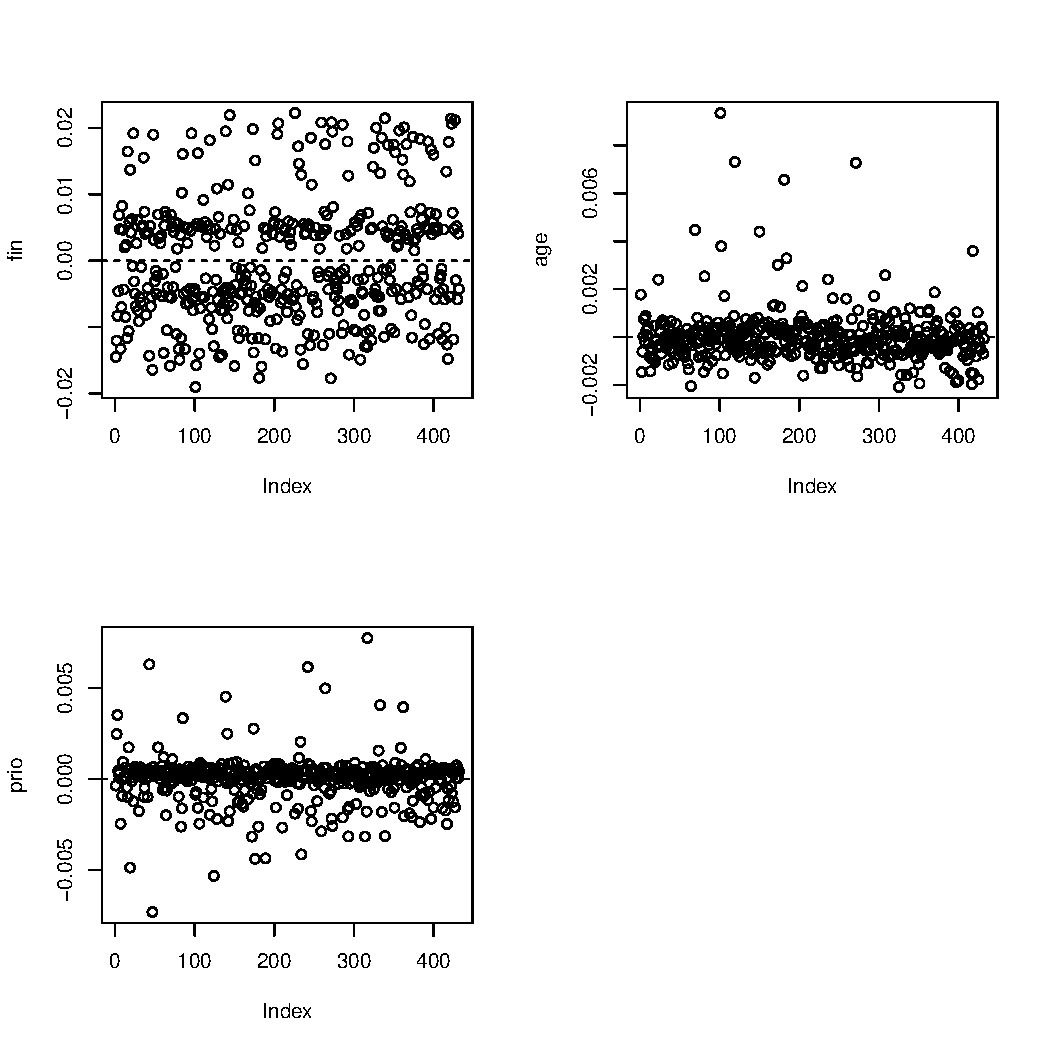
\includegraphics[width=\maxwidth]{figure/unnamed-chunk-102-1} 

\end{knitrout}
\caption{Diagnostic Plots for Proportional Hazard Assumption}
\label{Fig:hazard}
\rule{4in}{1pt}
\end{figure}

We are looking for systematic departures from the expected horizontal line. The plots confirm the result of the $cox.zph()$ function - we see string evidence of time dependent hazard for $age$ while the impact of $fin$ and $prio$ on the hazard rate seens more or less constant against time.

One way to accommodate non-proportional hazards is to build explicitely include interaction terms between covariates and time into the Cox regression model. For example, based on the diagnostics test and the plot, we can include a linear interaction of time and age in the model. As these interactions need to be treated as time-dependent covariates, we will need to include them in the long form data.
\begin{knitrout}
\definecolor{shadecolor}{rgb}{0.969, 0.969, 0.969}\color{fgcolor}\begin{kframe}
\begin{alltt}
\hlstd{mod.int} \hlkwb{<-} \hlkwd{coxph}\hlstd{(}\hlkwd{Surv}\hlstd{(start, stop, event)} \hlopt{~} \hlstd{fin} \hlopt{+} \hlstd{age} \hlopt{+} \hlstd{prio} \hlopt{+} \hlstd{age}\hlopt{:}\hlstd{stop,} \hlkwc{data} \hlstd{= rossi.long)}
\hlstd{mod.int}
\end{alltt}
\begin{verbatim}
## Call:
## coxph(formula = Surv(start, stop, event) ~ fin + age + prio + 
##     age:stop, data = rossi.long)
## 
##              coef exp(coef) se(coef)     z       p
## fin      -0.34856   0.70570  0.19023 -1.83 0.06690
## age       0.03228   1.03280  0.03943  0.82 0.41301
## prio      0.09818   1.10316  0.02726  3.60 0.00032
## age:stop -0.00383   0.99617  0.00147 -2.61 0.00899
## 
## Likelihood ratio test=36  on 4 df, p=2.85e-07
## n= 19809, number of events= 114
\end{verbatim}
\end{kframe}
\end{knitrout}

As the results show, the interaction between $age$ and $time$ is highly statistically significant with a negative coefficient. This means that the impact of $age$ on hazard rate reduces with passage of time. We can now check again whether including the interaction effect helped the model meet the assumption of proportional hazards. 

\begin{knitrout}
\definecolor{shadecolor}{rgb}{0.969, 0.969, 0.969}\color{fgcolor}\begin{kframe}
\begin{alltt}
\hlkwd{cox.zph}\hlstd{(mod.int)}
\end{alltt}
\begin{verbatim}
##              rho   chisq     p
## fin      -0.0068 0.00544 0.941
## age      -0.0471 0.36703 0.545
## prio     -0.0849 0.86449 0.352
## age:stop  0.0567 0.55701 0.455
## GLOBAL        NA 1.41901 0.841
\end{verbatim}
\end{kframe}
\end{knitrout}

All terms now show no statistically significant non-proportionality in hazards. Including the interaction term did help.

\subsection{Outliers}

Checking for outliers can be done using the \texttt{dfbeta} metric we have seen before in Linear Regression. Plot of $dfbeta$, as shown in Figure: \ref{Fig:outlier} can help us see any significant outliers. We can see that, compared to the coeficient values, corresponding dfbeta values are pretty small. We can, hence, conclude that the model does not suffer from significant outlier problem. 
\begin{figure}
\centering
\rule{4in}{1pt}
\begin{knitrout}
\definecolor{shadecolor}{rgb}{0.969, 0.969, 0.969}\color{fgcolor}\begin{kframe}
\begin{alltt}
\hlstd{dfbeta} \hlkwb{<-} \hlkwd{residuals}\hlstd{(mod.small,} \hlkwc{type} \hlstd{=} \hlstr{"dfbeta"}\hlstd{)}
\hlkwd{par}\hlstd{(}\hlkwc{mfrow} \hlstd{=} \hlkwd{c}\hlstd{(}\hlnum{2}\hlstd{,} \hlnum{2}\hlstd{))}
\hlkwa{for} \hlstd{(j} \hlkwa{in} \hlnum{1}\hlopt{:}\hlnum{3}\hlstd{) \{}
    \hlkwd{plot}\hlstd{(dfbeta[, j],} \hlkwc{ylab} \hlstd{=} \hlkwd{names}\hlstd{(}\hlkwd{coef}\hlstd{(mod.small))[j])}
    \hlkwd{abline}\hlstd{(}\hlkwc{h} \hlstd{=} \hlnum{0}\hlstd{,} \hlkwc{lty} \hlstd{=} \hlnum{2}\hlstd{)}
\hlstd{\}}
\end{alltt}
\end{kframe}
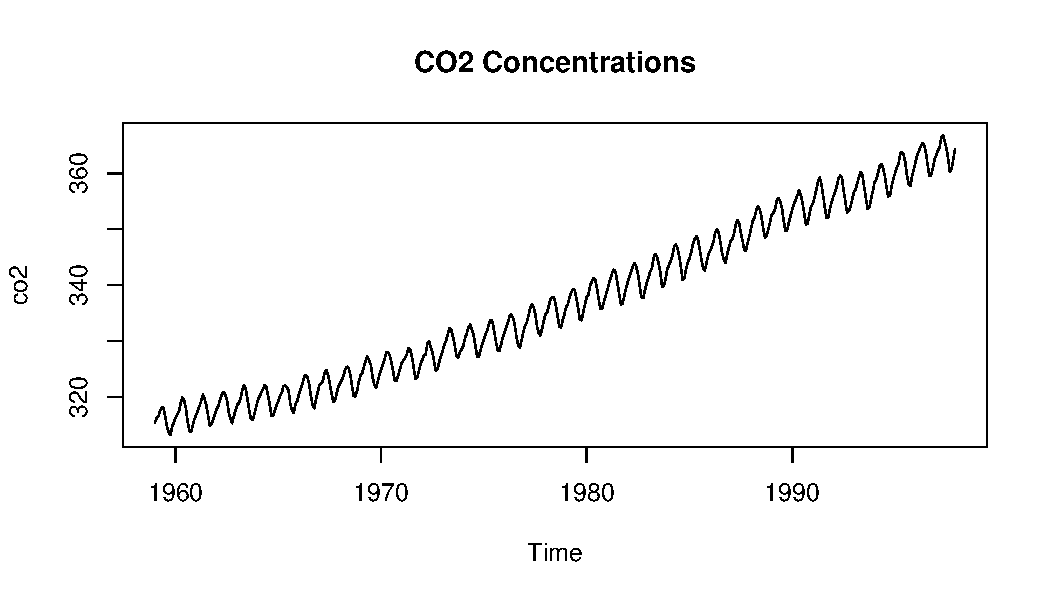
\includegraphics[width=\maxwidth]{figure/unnamed-chunk-105-1} 

\end{knitrout}
\caption{DFBeta Plots for Checking for Outliers}
\label{Fig:outlier}
\rule{4in}{1pt}
\end{figure}


\subsection{Acknowledgement}

Much of the material for this section has been taken from John Fox's excellent article "Cox Proportional-Hazards Regression for Survival Data" available at:\\ 
\small
\verb|https://socserv.socsci.mcmaster.ca/jfox/Books/Companion-1E/| 

\verb|appendix-cox-regression.pdf|. 
\normalsize
Code for converting data to long form has been taken from: \\ \verb|https://rpubs.com/kaz_yos/bio223-recidivism|. 

\chapterendsymbol


%\SweaveInput{TimeSeries.Rnw}

%\SweaveInput{PrinComp.Rnw}

\part{Machine Learning and Predictive Analytics}



% !Rnw root = AABase.Rnw

\chapter{Introduction to Machine Learning Algorithms}


\begin{flushright}

\textbf{\texttt{Big Data is like teenage sex: everyone talks about it, nobody really knows how to do it, everyone thinks everyone else is doing it, so everyone claims they are doing it.}}

\emph{-- Dan Ariely}

\end{flushright}

\vspace{12pt}

\chapterendsymbol




% !Rnw root = AABase.Rnw

\chapter{k-Nearest-Neighbors Classification}

\begin{flushright}

\textbf{\texttt{In God We Trust; All Others Must Bring Data}}

\emph{-- Willian Edwards Deming}

\end{flushright}

\vspace{12pt}


We will begin our exploration of machine learning algorithms today. We will begin with one of so called \emph{lazy learning} algorithms - Classification using Nearest Neighbors. It is essentially a process of discovery - classifying data by placing it in the category with the most similar or \emph{nearest} neighbors.

Despite the simple basic idea, nearest neighbor methods are extremely powerful and popular. Popular success examples like Netflix Challenge, Amazon Prediction Engine etc have used versions of this algorithm. This algorithm works best for classification tasks where relationships between features and target classes are complex and difficult to understand but the class types themselves are fairly homogeneous. If the groups are not well differentiated then nearest neighbor algorithm does not provide optimal results.

\section{kNN Algorithm}

kNN algorithm starts with a training dataset where records are already classified into target classes. We now attempt to classify a test dataset which is unclassified but otherwise has same features as the training dataset. For each record in the test dataset, kNN algorithm identifies \verb|k| records in the training data that are "nearest" or closest in features - here \verb|k| is an integer. The test record is assigned the class of the majority of the \verb|k| nearest neighbors.

kNN algorithm treats dataset features as coordinates in a multidimensional feature space. Two dimensional feature spaces can be easily visualized as a scatter plot. Higher dimensional features spaces are difficult to visualize but the essential idea remains the same. When trying to categorize a new record, we need to calculate its distance to records in the training dataset. Distances can be calculated as the Cartesian coordinate distance - also known as Euclidean Distance.

\section{Calculating Distance}

If we have two records $p$ and $q$; and $p_i$ and $q_i$ refer to the $i^th$ feature of $p$ and $q$ respectively; then the distance between $p$ and $q$ can be calculated as:

\[ dist(p, q) = \sqrt{(p_1 - q_1)^2 + (p_2 - q_2)^2 + ... + (p_n - q_n)^2} \]

Once we have distances with different records, we can sort them in increasing order. If we were to use $k = 1$ then we will just assign the record to the same category as the record with the smallest distance. If we use $k = 3$ then we look at the closest three neighbors and assign the record to the category that is most applicable within the three neighbors. 

\section{Choosing An Appropriate k}

Choosing an appropriate $k$ should balance between overfitting and underfitting the training data. This problem is commonly known as the \textbf{bias-variance tradeoff}. Choosing a large $k$ reduces the impact or variance caused by noisy data - but runs the risk of being biased against smaller but important patterns. Typically, smaller values allow for more complex decision boundaries that fit the training data better. In practice, choosing $k$ depends upon the difficulty of the classification task and the number of records in the training data. Typically, $k$ is set somewhere between 3 and 10. A common practice is to set $k$ equal to the square root of the number of records in training dataset.

\section{Rescaling Data for kNN}

As we depend on Euclidean Distance, the scale of variables matter a lot. Before we can apply kNN, we must transform variable to comparable scale. Following are the common methods of feature rescaling:

\begin{description}

\item [Min-Max Normalization] Convert all values on a 0 to 1 scale using the formula below to get normalized values.

\[X_{new} = \frac{X - min(X)}{max(X) - min(X)}   \]

\item [z-Score Standardization] Subtract mean value of the feature with the feature value and then divide by the standard deviation of the feature.

\[X_{new} = \frac{X - Mean(X)}{StdDev(X)} \]

z-Score essentially provides the number of standard deviations from the mean. Z-scores have a mean of 0 and distribution of 1. Unlike the normalized values above, z-score values are unbounded with a range of $-\infty$ to $\infty$.

\item [Dummy Coding] For nominal values, we use dummy coding of 1 or 0. If the feature has several levels then it will require several dummy variables (one less than the number of features). Dummy coding has the advantage of being on the same scale as normalized data.
\end{description}

\section{Illustrated Example: Breast Cancer Diagnosis}

We will illustrate kNN using "Breast Cancer Wisconsin Diagnostic" dataset from the UCI Machine Learning Repository. The dataset includes 569 examples of cancer biopsies each with 32 features. Of these 32, one is identification number and another is the cancer diagnosis (the target classification). Rest 30 are the features we need to use to figure out kNN classification.

\begin{knitrout}
\definecolor{shadecolor}{rgb}{0.969, 0.969, 0.969}\color{fgcolor}\begin{kframe}
\begin{alltt}
\hlcom{# Import Data}
\hlstd{wbcd} \hlkwb{<-} \hlkwd{read.csv}\hlstd{(}\hlstr{"wisc_bc_data.csv"}\hlstd{,} \hlkwc{stringsAsFactors} \hlstd{=} \hlnum{FALSE}\hlstd{)}
\hlcom{# str(wbcd) # Lets check what we have in this dataset Str command commented}
\hlcom{# for brevity in output}
\end{alltt}
\end{kframe}
\end{knitrout}

As the first variable $id$ is only a unique identifier, it is not likely to add any value to our model, so we can safely drop it from the dataset.
\begin{knitrout}
\definecolor{shadecolor}{rgb}{0.969, 0.969, 0.969}\color{fgcolor}\begin{kframe}
\begin{alltt}
\hlstd{wbcd} \hlkwb{<-} \hlstd{wbcd[}\hlopt{-}\hlnum{1}\hlstd{]}
\end{alltt}
\end{kframe}
\end{knitrout}

The second variable, $diagnosis$ is of significant interest as this is the target classification - in this case a variable with two values $B$ for Benign and $M$ for Malignant. We can check details of this variable. We will also convert the variable as a factor to recognize its essential nature.
\begin{knitrout}
\definecolor{shadecolor}{rgb}{0.969, 0.969, 0.969}\color{fgcolor}\begin{kframe}
\begin{alltt}
\hlkwd{table}\hlstd{(wbcd}\hlopt{$}\hlstd{diagnosis)}
\end{alltt}
\begin{verbatim}
## 
##   B   M 
## 357 212
\end{verbatim}
\begin{alltt}
\hlstd{wbcd}\hlopt{$}\hlstd{diagnosis} \hlkwb{<-} \hlkwd{factor}\hlstd{(wbcd}\hlopt{$}\hlstd{diagnosis,} \hlkwc{levels} \hlstd{=} \hlkwd{c}\hlstd{(}\hlstr{"B"}\hlstd{,} \hlstr{"M"}\hlstd{),} \hlkwc{labels} \hlstd{=} \hlkwd{c}\hlstd{(}\hlstr{"Benign"}\hlstd{,}
    \hlstr{"Malignant"}\hlstd{))}
\hlkwd{round}\hlstd{(}\hlkwd{prop.table}\hlstd{(}\hlkwd{table}\hlstd{(wbcd}\hlopt{$}\hlstd{diagnosis))} \hlopt{*} \hlnum{100}\hlstd{,} \hlnum{1}\hlstd{)}
\end{alltt}
\begin{verbatim}
## 
##    Benign Malignant 
##      62.7      37.3
\end{verbatim}
\end{kframe}
\end{knitrout}

\subsection{Rescaling the Data}

We need to now figure whether our data has a problem of differing scales. Exploring three variables here:
\begin{knitrout}
\definecolor{shadecolor}{rgb}{0.969, 0.969, 0.969}\color{fgcolor}\begin{kframe}
\begin{alltt}
\hlkwd{summary}\hlstd{(wbcd[}\hlkwd{c}\hlstd{(}\hlstr{"radius_mean"}\hlstd{,} \hlstr{"area_mean"}\hlstd{,} \hlstr{"smoothness_mean"}\hlstd{)])}
\end{alltt}
\begin{verbatim}
##   radius_mean       area_mean      smoothness_mean  
##  Min.   : 6.981   Min.   : 143.5   Min.   :0.05263  
##  1st Qu.:11.700   1st Qu.: 420.3   1st Qu.:0.08637  
##  Median :13.370   Median : 551.1   Median :0.09587  
##  Mean   :14.127   Mean   : 654.9   Mean   :0.09636  
##  3rd Qu.:15.780   3rd Qu.: 782.7   3rd Qu.:0.10530  
##  Max.   :28.110   Max.   :2501.0   Max.   :0.16340
\end{verbatim}
\end{kframe}
\end{knitrout}

We can clearly see that different variables differ significantly in their scale. So we will need to normalize our data so that we rescale variables to a standard range of values. We can write our own function for normalizing and then use $lapply$ to normalize our dataset.

\begin{knitrout}
\definecolor{shadecolor}{rgb}{0.969, 0.969, 0.969}\color{fgcolor}\begin{kframe}
\begin{alltt}
\hlstd{normalize} \hlkwb{<-} \hlkwa{function}\hlstd{(}\hlkwc{x}\hlstd{) \{}
    \hlkwd{return}\hlstd{((x} \hlopt{-} \hlkwd{min}\hlstd{(x))}\hlopt{/}\hlstd{(}\hlkwd{max}\hlstd{(x)} \hlopt{-} \hlkwd{min}\hlstd{(x)))}
\hlstd{\}}
\hlstd{wbcd_n} \hlkwb{<-} \hlkwd{as.data.frame}\hlstd{(}\hlkwd{lapply}\hlstd{(wbcd[}\hlnum{2}\hlopt{:}\hlnum{31}\hlstd{], normalize))}
\hlkwd{summary}\hlstd{(wbcd_n[}\hlkwd{c}\hlstd{(}\hlstr{"radius_mean"}\hlstd{,} \hlstr{"area_mean"}\hlstd{,} \hlstr{"smoothness_mean"}\hlstd{)])}
\end{alltt}
\begin{verbatim}
##   radius_mean       area_mean      smoothness_mean 
##  Min.   :0.0000   Min.   :0.0000   Min.   :0.0000  
##  1st Qu.:0.2233   1st Qu.:0.1174   1st Qu.:0.3046  
##  Median :0.3024   Median :0.1729   Median :0.3904  
##  Mean   :0.3382   Mean   :0.2169   Mean   :0.3948  
##  3rd Qu.:0.4164   3rd Qu.:0.2711   3rd Qu.:0.4755  
##  Max.   :1.0000   Max.   :1.0000   Max.   :1.0000
\end{verbatim}
\end{kframe}
\end{knitrout}

As we can now see, our three variables in question are now distributed on a standard scale; and are comparable to each other as far as euclidean distance is concerned.

\subsection{Dividing Data Into Training and Testing Sets}

Alright - now we need to train our model. Of course, we shouldn't use the entire dataset to train as then we will have no way to test the model. Lets keep 100 observations as the test dataset and use the rest for training.
\begin{knitrout}
\definecolor{shadecolor}{rgb}{0.969, 0.969, 0.969}\color{fgcolor}\begin{kframe}
\begin{alltt}
\hlstd{wbcd_train} \hlkwb{<-} \hlstd{wbcd_n[}\hlnum{1}\hlopt{:}\hlnum{469}\hlstd{, ]}
\hlstd{wbcd_test} \hlkwb{<-} \hlstd{wbcd_n[}\hlnum{470}\hlopt{:}\hlnum{569}\hlstd{, ]}
\end{alltt}
\end{kframe}
\end{knitrout}

We would also want to extract the target variable in factors. These factors would be useful for us in a little bit when we train and test out model.
\begin{knitrout}
\definecolor{shadecolor}{rgb}{0.969, 0.969, 0.969}\color{fgcolor}\begin{kframe}
\begin{alltt}
\hlstd{wbcd_train_labels} \hlkwb{<-} \hlstd{wbcd[}\hlnum{1}\hlopt{:}\hlnum{469}\hlstd{,} \hlnum{1}\hlstd{]}
\hlstd{wbcd_test_labels} \hlkwb{<-} \hlstd{wbcd[}\hlnum{470}\hlopt{:}\hlnum{569}\hlstd{,} \hlnum{1}\hlstd{]}
\end{alltt}
\end{kframe}
\end{knitrout}

\subsection{Running the Model}

Now is the time to train our model on the training data. We will need a package named $class$. Class package includes several classification algorithms.
\begin{knitrout}
\definecolor{shadecolor}{rgb}{0.969, 0.969, 0.969}\color{fgcolor}\begin{kframe}
\begin{alltt}
\hlcom{# install.packages('class') #Commented}
\hlkwd{library}\hlstd{(class)}
\end{alltt}
\end{kframe}
\end{knitrout}

We will use the $knn()$ function. The function call is pretty simple. It needs a training dataset, a testing dataset, a factor vector with the classification for each row in training data and an integer value corresponding to the number of nearest neighbors $k$. Since we have 469 observations in the training data, we might want to start with $k = 21$ as it is closest odd number to square root of 469. The function returns a factor vector of predicted values for each record in the test dataset.

\begin{knitrout}
\definecolor{shadecolor}{rgb}{0.969, 0.969, 0.969}\color{fgcolor}\begin{kframe}
\begin{alltt}
\hlstd{wbcd_test_pred} \hlkwb{<-} \hlkwd{knn}\hlstd{(}\hlkwc{train} \hlstd{= wbcd_train,} \hlkwc{test} \hlstd{= wbcd_test,} \hlkwc{cl} \hlstd{= wbcd_train_labels,}
    \hlkwc{k} \hlstd{=} \hlnum{21}\hlstd{)}
\end{alltt}
\end{kframe}
\end{knitrout}

\subsection{Model Accuracy}

Alright - so we have run a model - is it any good? We should evaluate model performance. In this case it is easy since we already know what should have been the classification. The $CrossTable()$ function in the $gmodels$ package is a good choice to do this calculation.
\begin{knitrout}
\definecolor{shadecolor}{rgb}{0.969, 0.969, 0.969}\color{fgcolor}\begin{kframe}
\begin{alltt}
\hlcom{# install.packages('gmodels') #Comments}
\hlkwd{library}\hlstd{(gmodels)}
\hlkwd{CrossTable}\hlstd{(}\hlkwc{x} \hlstd{= wbcd_test_labels,} \hlkwc{y} \hlstd{= wbcd_test_pred,} \hlkwc{prop.chisq} \hlstd{=} \hlnum{FALSE}\hlstd{)}
\end{alltt}
\begin{verbatim}
## 
##  
##    Cell Contents
## |-------------------------|
## |                       N |
## |           N / Row Total |
## |           N / Col Total |
## |         N / Table Total |
## |-------------------------|
## 
##  
## Total Observations in Table:  100 
## 
##  
##                  | wbcd_test_pred 
## wbcd_test_labels |    Benign | Malignant | Row Total | 
## -----------------|-----------|-----------|-----------|
##           Benign |        61 |         0 |        61 | 
##                  |     1.000 |     0.000 |     0.610 | 
##                  |     0.968 |     0.000 |           | 
##                  |     0.610 |     0.000 |           | 
## -----------------|-----------|-----------|-----------|
##        Malignant |         2 |        37 |        39 | 
##                  |     0.051 |     0.949 |     0.390 | 
##                  |     0.032 |     1.000 |           | 
##                  |     0.020 |     0.370 |           | 
## -----------------|-----------|-----------|-----------|
##     Column Total |        63 |        37 |       100 | 
##                  |     0.630 |     0.370 |           | 
## -----------------|-----------|-----------|-----------|
## 
## 
\end{verbatim}
\end{kframe}
\end{knitrout}

As we can see, there were 69 true negative cases - the mass was benign - and the kNN algorithm correctly identified each of the cases. There were 37 true positive cases where the model and the test data agree on identification of malignant cases. The model presents 2 false negatives and 0 false positives. So we have a 98\% accuracy - only two cases were wrongly classified.

\subsection{Improving the Model with z-Scores}

We have two ways to see if we can improve this model - we can try different values of $k$ and try a different rescaling technique. Lets start by using the z-score as the rescaling method. We can use the $scale()$ function for this.
\begin{knitrout}
\definecolor{shadecolor}{rgb}{0.969, 0.969, 0.969}\color{fgcolor}\begin{kframe}
\begin{alltt}
\hlstd{wbcd_z} \hlkwb{<-} \hlkwd{as.data.frame}\hlstd{(}\hlkwd{scale}\hlstd{(wbcd[}\hlopt{-}\hlnum{1}\hlstd{]))}
\end{alltt}
\end{kframe}
\end{knitrout}

We follow the same process as before for creating training and testing data.
\begin{knitrout}
\definecolor{shadecolor}{rgb}{0.969, 0.969, 0.969}\color{fgcolor}\begin{kframe}
\begin{alltt}
\hlstd{wbcd_train} \hlkwb{<-} \hlstd{wbcd_z[}\hlnum{1}\hlopt{:}\hlnum{469}\hlstd{, ]}
\hlstd{wbcd_test} \hlkwb{<-} \hlstd{wbcd_z[}\hlnum{470}\hlopt{:}\hlnum{569}\hlstd{, ]}
\end{alltt}
\end{kframe}
\end{knitrout}

We are ready to run a new model now.
\begin{knitrout}
\definecolor{shadecolor}{rgb}{0.969, 0.969, 0.969}\color{fgcolor}\begin{kframe}
\begin{alltt}
\hlstd{wbcd_test_pred} \hlkwb{<-} \hlkwd{knn}\hlstd{(}\hlkwc{train} \hlstd{= wbcd_train,} \hlkwc{test} \hlstd{= wbcd_test,} \hlkwc{cl} \hlstd{= wbcd_train_labels,}
    \hlkwc{k} \hlstd{=} \hlnum{21}\hlstd{)}
\end{alltt}
\end{kframe}
\end{knitrout}

Let us see how we did this time.
\begin{knitrout}
\definecolor{shadecolor}{rgb}{0.969, 0.969, 0.969}\color{fgcolor}\begin{kframe}
\begin{alltt}
\hlkwd{CrossTable}\hlstd{(}\hlkwc{x} \hlstd{= wbcd_test_labels,} \hlkwc{y} \hlstd{= wbcd_test_pred,} \hlkwc{prop.chisq} \hlstd{=} \hlnum{FALSE}\hlstd{)}
\end{alltt}
\begin{verbatim}
## 
##  
##    Cell Contents
## |-------------------------|
## |                       N |
## |           N / Row Total |
## |           N / Col Total |
## |         N / Table Total |
## |-------------------------|
## 
##  
## Total Observations in Table:  100 
## 
##  
##                  | wbcd_test_pred 
## wbcd_test_labels |    Benign | Malignant | Row Total | 
## -----------------|-----------|-----------|-----------|
##           Benign |        61 |         0 |        61 | 
##                  |     1.000 |     0.000 |     0.610 | 
##                  |     0.924 |     0.000 |           | 
##                  |     0.610 |     0.000 |           | 
## -----------------|-----------|-----------|-----------|
##        Malignant |         5 |        34 |        39 | 
##                  |     0.128 |     0.872 |     0.390 | 
##                  |     0.076 |     1.000 |           | 
##                  |     0.050 |     0.340 |           | 
## -----------------|-----------|-----------|-----------|
##     Column Total |        66 |        34 |       100 | 
##                  |     0.660 |     0.340 |           | 
## -----------------|-----------|-----------|-----------|
## 
## 
\end{verbatim}
\end{kframe}
\end{knitrout}

Well - the new model is actually a little bit worse. We now have 95\% accuracy. False negatives actually increased - and that is actually a worse mistake to make than a false positive - so all in all - not a change that worked for us.

\subsection{Trying Different k Values}

Okay - we still have the option of trying different $k$ values. Following are the results for different $k$ values using normalized training data.

\begin{figure}[h]
\centering
\begin{tabular}{| c | c | c | c |}
\hline 
k value & False Positives & False Negatives & Accuracy Percentage \\
\hline
1 & 1 & 3 & 96\% \\
5 & 2 & 0 & 98\% \\
11 & 3 & 0 & 97\% \\
15 & 3 & 0 & 97\% \\
21 & 2 & 0 & 98\% \\
27 & 4 & 0 & 96\% \\
\hline \hline
\end{tabular}
\caption{Different k Values}
\label{Fig:knn}
\rule{4in}{1pt}
\end{figure}

What do you think is the best model. $k = 1$ is better for avoiding false negatives. Original $k = 21$ was better as far as overall accuracy is concerned.

\chapterendsymbol




% !Rnw root = AABase.Rnw

\chapter{k-Means Clustering}

\begin{flushright}

\textbf{\texttt{In God We Trust; All Others Must Bring Data}}

\emph{-- Willian Edwards Deming}

\end{flushright}

\vspace{12pt}

\chapterendsymbol




% !Rnw root = AABase.Rnw

\chapter{Finding Patterns using Association Rules}

\begin{flushright}

\textbf{\texttt{In God We Trust; All Others Must Bring Data}}

\emph{-- Willian Edwards Deming}

\end{flushright}

\vspace{12pt}

\chapterendsymbol




% !Rnw root = AABase.Rnw

\chapter{Classification using Support Vector Machines}

\begin{flushright}

\textbf{\texttt{In God We Trust; All Others Must Bring Data}}

\emph{-- Willian Edwards Deming}

\end{flushright}

\vspace{12pt}

\chapterendsymbol




% !Rnw root = AABase.Rnw

\chapter{Deep Learning using Neural Networks}

\begin{flushright}

\textbf{\texttt{In God We Trust; All Others Must Bring Data}}

\emph{-- Willian Edwards Deming}

\end{flushright}

\vspace{12pt}

\chapterendsymbol




% !Rnw root = AABase.Rnw

\chapter{Decision Trees and Random Forests}

\begin{flushright}

\textbf{\texttt{In God We Trust; All Others Must Bring Data}}

\emph{-- Willian Edwards Deming}

\end{flushright}

\vspace{12pt}

\chapterendsymbol



\part{Putting It All Together}



% !Rnw root = AABase.Rnw

\chapter{Improving and Combining Models}

\begin{flushright}

\textbf{\texttt{In God We Trust; All Others Must Bring Data}}

\emph{-- Willian Edwards Deming}

\end{flushright}

\vspace{12pt}

\chapterendsymbol




% !Rnw root = AABase.Rnw

\chapter{Some Last Words}

\begin{flushright}

\textbf{\texttt{Torture the data, and it will confess to anything.}}

\emph{-- Ronald Coase, Economics Nobel Laureate}

\end{flushright}

\vspace{12pt}


\chapterendsymbol



\part{Appendices, Bibliography and Index}

\appendix



% !Rnw root = AABase.Rnw

\chapter{Key References}

\begin{flushright}
\texttt{In God We Trust; All Others Must Bring Data}

\emph{-- Willian Edwards Deming}
\end{flushright}

\vspace{12pt}


If you are new to R and data anaytics (or if it has been a while and you wish to refresh your mind), these are the key references you should start with:

\section{Beginner Level Resources}


\section{Intermediate Level Resources}


\section{Advanced Resources}

\chapterendsymbol




% !Rnw root = AABase.Rnw

\chapter{Data Analysis Example}

First, lets make sure that we have R/RStudio set up to work in the right directory. You can type the command \rcommand{getwd} to see which directory is R/RStudio working in right now:

\begin{knitrout}
\definecolor{shadecolor}{rgb}{0.969, 0.969, 0.969}\color{fgcolor}\begin{kframe}
\begin{alltt}
\hlkwd{getwd}\hlstd{()}
\end{alltt}
\begin{verbatim}
## [1] "/Users/sankum/Documents/5AABook"
\end{verbatim}
\end{kframe}
\end{knitrout}

If you wish to change the directory you want to work in (remember this is the directory where R/RStudio will save all outputs), then you can do so using the command \rcommand{setwd} and specifying the directory address. For example, the command below will make \verb|"c:\users\sankum"| the working directory. 

\begin{knitrout}
\definecolor{shadecolor}{rgb}{0.969, 0.969, 0.969}\color{fgcolor}\begin{kframe}
\begin{alltt}
\hlcom{# setwd('c:/users/sankum') #Command disabled}
\end{alltt}
\end{kframe}
\end{knitrout}

Download the data file (available at: \href{https://umich.box.com/s/xtpp98qygojc0fh14vhlvdr6nzsa47a2}{Link to Data File}) and save it in the working directory for R/RStudio using the filename \texttt{nycflightsjan13.csv}. Now, we need to get the data that we want to analyze into the R environment. We will do so by importing the data file into R using the following command \index{R Commands!read.csv}:

\begin{knitrout}
\definecolor{shadecolor}{rgb}{0.969, 0.969, 0.969}\color{fgcolor}\begin{kframe}
\begin{alltt}
\hlstd{nycdata} \hlkwb{<-} \hlkwd{read.csv}\hlstd{(}\hlstr{"nycflightsjan13.csv"}\hlstd{)}
\end{alltt}
\end{kframe}
\end{knitrout}

There are a lot of things going on in the command above. Here are the key elements: \texttt{"<-"} is called the \textbf{Assignment Operator}\index{Key Concepts!Assignment Operator} - it takes the value on its left and assigns that value to the object on its right. On the right of the assignment operator, we have the R function \texttt{read.csv()} which reads a CSV or Comma Separated Values files. On the left we have a \textbf{Data Frame} that we are calling \texttt{nycdata}. 

We have used several technical terms that we should define before going forward:\\
\textbf{Operators} are part of R language and perform certain \textit{operations}. For example, as we saw, the assignment operators assigns the value from its left side to the object on its right side.\\
\textbf{Objects} are basic building blocks of the R language that may contain both data and logic. R is an \textbf{Object Oriented Language} which means that it is organized around objects and their interactions.\\
\textbf{Data Frame} is one of various types of objects in R that is used to store data. Data frames store data in neat rows and columns (like an Excel table) which makes them easy to use. Typically, columns contain different data fields and rows contain different observations of those data fields.\\
\textbf{Functions} Function are pieces of code that perform a task and then return (or give back) a value. Functions (or their counterpart Subs - which also perform a task but do not return a value) can be identified by the \texttt{()} characters. When the function needs some information to perform the task, then that information is provided to the function by placing them inside \texttt{()} characters (as in the example above of \texttt{read.csv()} function.\\ 
\textbf{read.csv()} is one various types of functions that perform the task of importing data into an R object. This function reads a CSV file and outputs the contents of the file in the data frame format.

So, we have used the \texttt{read.csv()} function to import data contained in the \texttt{nycflightsjan13.csv} file into the data frame named \texttt{nycdata}. Let's first peek inside this data frame using the \texttt{head()} \index{R Commands!head} function that shows first few lines of data.

\begin{knitrout}
\definecolor{shadecolor}{rgb}{0.969, 0.969, 0.969}\color{fgcolor}\begin{kframe}
\begin{alltt}
\hlkwd{head}\hlstd{(nycdata)}
\end{alltt}
\begin{verbatim}
##   X year month day dep_time dep_delay arr_time arr_delay carrier tailnum
## 1 1 2013     1   1      517         2      830        11      UA  N14228
## 2 2 2013     1   1      533         4      850        20      UA  N24211
## 3 3 2013     1   1      542         2      923        33      AA  N619AA
## 4 4 2013     1   1      544        -1     1004       -18      B6  N804JB
## 5 5 2013     1   1      554        -6      812       -25      DL  N668DN
## 6 6 2013     1   1      554        -4      740        12      UA  N39463
##   flight origin dest air_time distance hour minute
## 1   1545    EWR  IAH      227     1400    5     17
## 2   1714    LGA  IAH      227     1416    5     33
## 3   1141    JFK  MIA      160     1089    5     42
## 4    725    JFK  BQN      183     1576    5     44
## 5    461    LGA  ATL      116      762    5     54
## 6   1696    EWR  ORD      150      719    5     54
\end{verbatim}
\end{kframe}
\end{knitrout}

The data shows various information about all the flights departing from one of NYC airports in Jan 2013. Different data fields labels (first row of the data frame) are self explanatory. 

If we want to know how many rows and columns there are in our data frame, then we can use the \texttt{nrow()} and \texttt{ncol()} \index{R Commands!nrow} \index{R Commands!ncol} function. Note that as shown below, you can run multiple R command on the same line by separating them using the end-of-command character \texttt{";"}.

\begin{knitrout}
\definecolor{shadecolor}{rgb}{0.969, 0.969, 0.969}\color{fgcolor}\begin{kframe}
\begin{alltt}
\hlkwd{nrow}\hlstd{(nycdata)}
\end{alltt}
\begin{verbatim}
## [1] 27004
\end{verbatim}
\begin{alltt}
\hlkwd{ncol}\hlstd{(nycdata)}
\end{alltt}
\begin{verbatim}
## [1] 17
\end{verbatim}
\end{kframe}
\end{knitrout}

We can calculate average arrival delay using the \texttt{mean()} \index{R Commands!mean} function:

\begin{knitrout}
\definecolor{shadecolor}{rgb}{0.969, 0.969, 0.969}\color{fgcolor}\begin{kframe}
\begin{alltt}
\hlkwd{mean}\hlstd{(nycdata}\hlopt{$}\hlstd{arr_delay,} \hlkwc{na.rm} \hlstd{=} \hlnum{TRUE}\hlstd{)}
\end{alltt}
\begin{verbatim}
## [1] 6.129972
\end{verbatim}
\end{kframe}
\end{knitrout}

We did two new things - we used the \verb|"$"| character to access an column inside the data frame. Essentially, \verb|X$Y| refers to the \texttt{Y} column in the data frame \texttt{X}. We asked the \texttt{mean()} function to calculate the average of the \verb|arr_delay| column in \texttt{nycdata} data frame. However, there are many values in the \verb|arr_delay| column that are missing (think of an empty cell in Excel). These missing values are coded as \texttt{NA} in R and the \texttt{mean()} function has an optional input \texttt{na.rm} which allows you to specify how you would want to consider these \texttt{NA} values. \texttt{na.rm=TRUE} tells R that it should remove (hence the term \texttt{rm}) any \texttt{na} values from the calculations.

Similar to the example above, we can calculate other descriptive statistics such as Median, Minimum, Maximum, Standard Deviation, Inter-Quartile Range etc.\index{R Commands!median}\index{R Commands!IQR}

\begin{knitrout}
\definecolor{shadecolor}{rgb}{0.969, 0.969, 0.969}\color{fgcolor}\begin{kframe}
\begin{alltt}
\hlkwd{median}\hlstd{(nycdata}\hlopt{$}\hlstd{arr_delay,} \hlkwc{na.rm} \hlstd{=} \hlnum{TRUE}\hlstd{)}
\end{alltt}
\begin{verbatim}
## [1] -3
\end{verbatim}
\begin{alltt}
\hlkwd{IQR}\hlstd{(nycdata}\hlopt{$}\hlstd{arr_delay,} \hlkwc{na.rm} \hlstd{=} \hlnum{TRUE}\hlstd{)}
\end{alltt}
\begin{verbatim}
## [1] 28
\end{verbatim}
\end{kframe}
\end{knitrout}

\begin{figure}
\rule{4in}{1pt}
\centering
\begin{knitrout}
\definecolor{shadecolor}{rgb}{0.969, 0.969, 0.969}\color{fgcolor}\begin{kframe}
\begin{alltt}
\hlkwd{hist}\hlstd{(nycdata}\hlopt{$}\hlstd{arr_delay[nycdata}\hlopt{$}\hlstd{arr_delay} \hlopt{<} \hlnum{300}\hlstd{])}
\end{alltt}
\end{kframe}
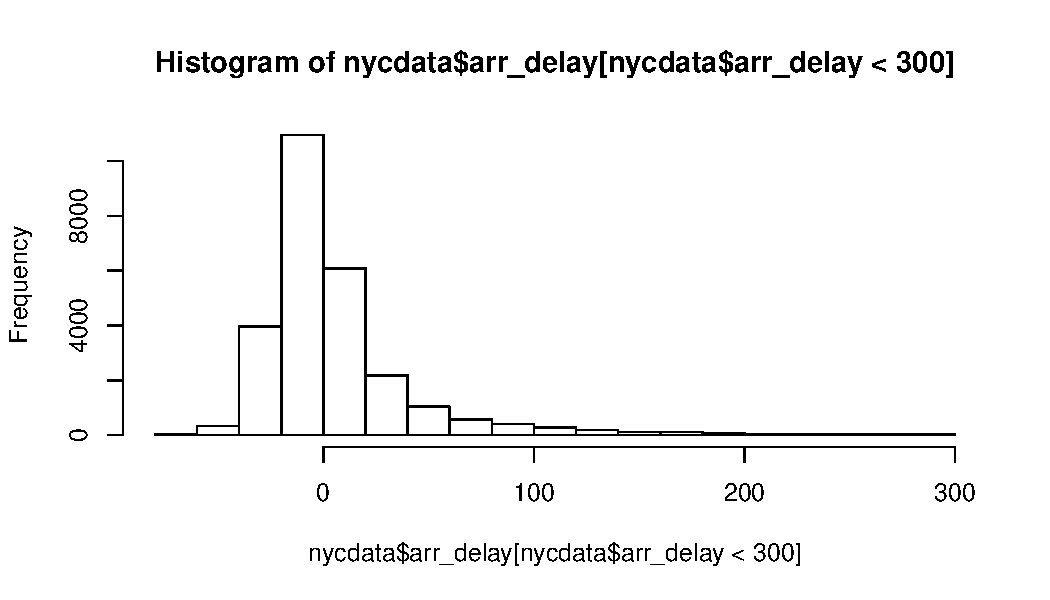
\includegraphics[width=\maxwidth]{figure/unnamed-chunk-127-1} 

\end{knitrout}
\caption{Example of a Histogram}
\label{fig:hist}
\rule{4in}{1pt}
\end{figure}

We can easily plot our data in R. The code for Figure \ref{fig:hist} creates a histogram using the \texttt{hist()} \index{R Commands!hist} function. We gave this function the \verb|arr_delay| column from the data frame but to make the plot more readable, we \textbf{filtered} the data to only show values that are less than 300. As shown above, the filtering condition is presented inside \verb|[]| characters.

The plot shows that most of the flights that departed from NYC in Jan 2013 reached their destination without any significant delay. However, there might be differences between airlines - we would want to see average arrival delays calculated for each different airlines.

\begin{knitrout}
\definecolor{shadecolor}{rgb}{0.969, 0.969, 0.969}\color{fgcolor}\begin{kframe}
\begin{alltt}
\hlstd{delaybycarrier} \hlkwb{<-} \hlkwd{tapply}\hlstd{(nycdata}\hlopt{$}\hlstd{arr_delay, nycdata}\hlopt{$}\hlstd{carrier, mean,} \hlkwc{na.rm} \hlstd{=} \hlnum{TRUE}\hlstd{)}
\hlstd{delaybycarrier}
\end{alltt}
\begin{verbatim}
##          9E          AA          AS          B6          DL          EV 
##  10.2074324   0.9823789   8.9677419   4.7171992  -4.4046512  25.1601917 
##          F9          FL          HA          MQ          OO          UA 
##  21.8305085   3.3179012  27.4838710   7.8837948 107.0000000   3.1755991 
##          US          VX          WN          YV 
##   1.4311454 -15.2802548   5.8862944  13.7692308
\end{verbatim}
\end{kframe}
\end{knitrout}

Again we did some interesting things here. We calculated the average of \verb|arr_delay| column for each \texttt{carrier} using the \texttt{tapply()} \index{R Commands!tapply} function. We saved the output in an object named \texttt{delaybycarrier}. When we type just the object name by itself then R essentially prints out the contents of the object - which in this case consists of carrier names and corresponding average arrival delay. We can see that the carrier \texttt{VX} had the lowest arrival delay in Jan 2013 while the carrier \texttt{OO} had the highest.

To illustrate the point further, we can make a barplot using the \texttt{barplot()} \index{R Commands!barplot} function (Figure \ref{fig:bar}) - not much different than the $hist()$ function before. 

\begin{figure}
\centering
\rule{6in}{1pt}
\begin{knitrout}
\definecolor{shadecolor}{rgb}{0.969, 0.969, 0.969}\color{fgcolor}\begin{kframe}
\begin{alltt}
\hlkwd{barplot}\hlstd{(delaybycarrier)}
\end{alltt}
\end{kframe}
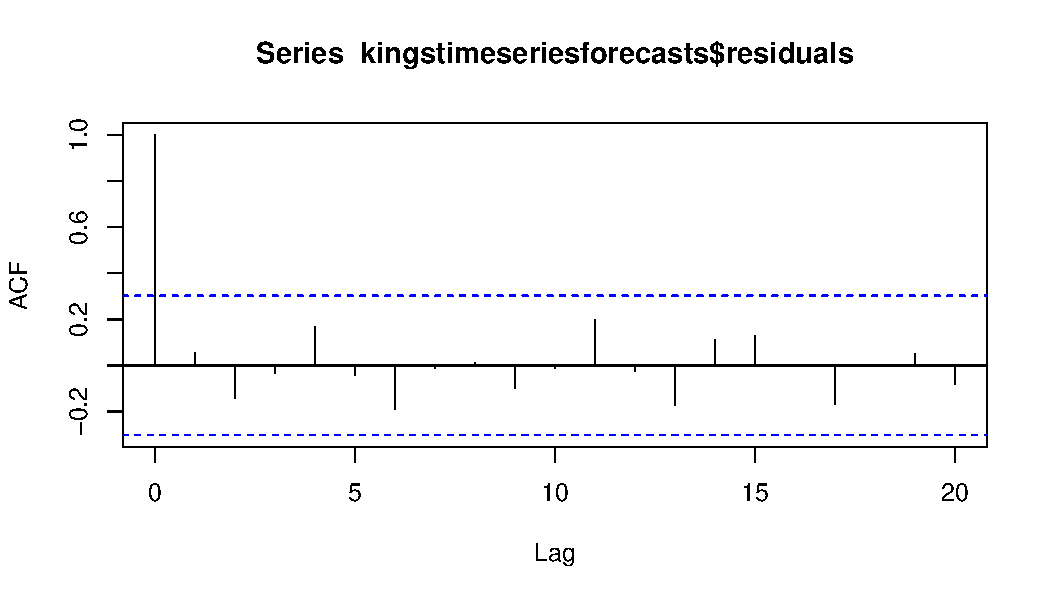
\includegraphics[width=\maxwidth]{figure/unnamed-chunk-129-1} 

\end{knitrout}
\caption{Barplot of NYC Flights Data}
\label{fig:bar}
\rule{6in}{1pt}
\end{figure}

We will end our data analysis example with an example of loading a new package and using that to create a new column in the dataset. R's power and versatility comes from various extensions (called $packages$) created by volunteers. These packages need to be installed and then loaded into memory for them to be used. We will install the $dplyr$ \index{Packages!dplyr} \index{R Commands!install.packages} \index{R Commands!library} package and load it using the following commands.

\begin{knitrout}
\definecolor{shadecolor}{rgb}{0.969, 0.969, 0.969}\color{fgcolor}\begin{kframe}
\begin{alltt}
\hlcom{# install.packages('dplyr', repos='https://cran.rstudio.com/')}
\hlkwd{library}\hlstd{(plyr)}
\hlkwd{library}\hlstd{(dplyr)}
\end{alltt}
\end{kframe}
\end{knitrout}

Let's say we want to calculate the speed of all the flights in the NYC Flights dataset we looked at earlier. We can use the \texttt{mutate} \index{R Commands!mutate} command in the \texttt{dplyr} package to do so.

\begin{knitrout}
\definecolor{shadecolor}{rgb}{0.969, 0.969, 0.969}\color{fgcolor}\begin{kframe}
\begin{alltt}
\hlstd{nycdata} \hlkwb{<-} \hlkwd{mutate}\hlstd{(nycdata,} \hlkwc{avgspeed} \hlstd{= distance}\hlopt{/}\hlstd{air_time)}
\end{alltt}
\end{kframe}
\end{knitrout}

You can use the \texttt{head()} function we used earlier to check whether the new column has in fact been created. Note that we could have done the above task without going to \texttt{dplyr} at all.

\begin{knitrout}
\definecolor{shadecolor}{rgb}{0.969, 0.969, 0.969}\color{fgcolor}\begin{kframe}
\begin{alltt}
\hlstd{nycdata}\hlopt{$}\hlstd{newspeed} \hlkwb{=} \hlstd{nycdata}\hlopt{$}\hlstd{distance}\hlopt{/}\hlstd{nycdata}\hlopt{$}\hlstd{air_time}
\end{alltt}
\end{kframe}
\end{knitrout}

You can use either of the above two approach - all depends upon your preference. This brings us to our concluding thought of this demo. There are several (sometimes hundreds) of different ways to doing a task in R. Some are more suitable to the given context than others. However, it is up to you choose which to become expert on, which to know peripherally and which to ignore. Each person's interaction and experience with R is unique to that person and his/her choices. I hope this demo has given you an idea of the power, depth and versatility of R and has made you interested in the deep dives into different aspects of R that are about to come in following chapter.  





% !Rnw root = AABase.Rnw

\chapter{Syllabus for TO414 Fall 2016}

\begin{flushright}

\textbf{\texttt{In God We Trust; All Others Must Bring Data}}

\emph{-- Willian Edwards Deming}

\end{flushright}

\vspace{12pt}


\section{Course Description}

We live in a world awash in data. Companies are increasingly turning to data analytics to extract a competitive edge from data, especially large, complex datasets often called "Big Data". However, companies are increasingly facing the challenge posed by the scarcity of analytical talent - people who can turn data into better decisions, people who can extract insights and information from data. There is growing demand for professionals with strong quantitative skills combined with an understanding of how data analytic techniques can be applied to business contexts and managerial decision making. To help students succeed in this growing field, this course teaches advanced analytical, statistical and data mining tools with an applied focus. 

The main focus of this course is to prepare students to model and manage business decisions with data analytics and decision models using real life case contexts and datasets.  By the end of this course students will have a better understanding of processes, methodologies and tools used to transform the large amount of business data available into useful information and support business decision making. The course will focus on extracting actionable business intelligence by analyzing traditional business data as well as more recently available datasets such as social media, crowdsourcing and recommendation engines. The course focuses on the powerful, open source (and hence free) data analysis environment R – prior experience with R is NOT required. As this is an applied course, the focus is on application of various statistical and analytical tools and the student is assumed to be familiar with basic statistics at TO 301 level. A working knowledge of spreadsheet applications like MS-Excel is assumed.


\section{Class Details}
\begin{itemize}
\item Class Schedule: Tue/Thu 10AM-11:30AM, R1240
\item Instructor Information: Dr. Sanjeev Kumar, R3443, sankum@umich.edu, @theSanjeev, 734-615-7064
\item Office Hours: TBD, by appointment, my office is always open for my students - come by \emph{anytime}.
\item Class Materials: Distributed through the Canvas site for the course, through clarifyR GitHub page and through http://clarifyR.com.
\item Teaching Assistants: Class has two dedicated teaching assistants with extensive experience with R. TAs will attend all classes and help students with class exercises. TAs will also hold office hours (times TBD) to help students with individual and group assignments.
\end{itemize}

\section{Course Materials}

All course materials will be distributed through the Canvas site for the course. Each class will usually have a reading assigned to it and a dataset for students to work on. There is no assigned textbook for the course - the instructor has developed a custom textbook for the class. All datasets, reading materials, assignments and exercises will be distributed through the \emph{clarifyR} packages available on GitHub as an R package.

The class will require students to bring their own laptops to class - any Windows, Mac or Linux machines are fine. However, Chromebooks are not suitable for the class as it is not usually possible to run R/RStudio on Chromebooks effectively on them. In case some students do not have access to suitable laptops or in case of students facing temporary technical problems, about 10 laptops will be provided during each class session for students to use.

Apart from the Canvas site for the course, course material will also be available through http://clarifyR.com, the website for the custom textbook and custom R package for the course available through GitHub.

\section{Course Grading}
\begin{itemize}
\item In-Class Quizzes, Exercises, Assignments and Class Participation: 20\%

\item Individual Homework Assignments: 10 x 4\% each = 40\%
\begin{enumerate}
    \item Basic tasks in R, creating RMarkdown documents and RShiny apps
    \item Data manipulation, data cleaning
    \item Descriptive statistics, basic R graphics
    \item Linear regression
    \item Logistic regression
    \item Principal Component / Factor analysis
    \item Classification using kNN
    \item Clustering using k-Means-Clustering
    \item Classification using black box models
    \item Decision Trees, Random Forests
\end{enumerate}
\item Group Projects: 20\%. Group project deliverable include a data analysis report (RMD file and html/pdf output, RShiny dashboard) and a 10 min class presentation for Group Project 2.  
\begin{itemize}
    \item Group Project 1: 7\% for Project Report on Data exploration, cleaning, visualization and descriptive statistics
    \item Group Project 2: 7\% for Project Report + 6\% for Project Presentation on Integrated Models for Predictive Analytics - building the best predictive machine learning model
\end{itemize}    
\item Individual Final Assessment: 20\%
\end{itemize}    

Course grading will follow the usual Ross grading curve for elective courses. Typical grade curve allows for less than 60\% of students in A range, less than 90\% of students in B and above range and at least 10\% of students in B-Minus and below. All efforts will be made to assign students as high a grade as possible within the Ross elective grade curve.

\section{Class Schedule}

All individual assignments are typically due before class in one weeks time. Group projects are typically due before class in two weeks time. The class schedule below provides specific details for submission due dates. Further details will be posted on the Canvas site for the course.

\subsection{Module 1: Setting the Foundation}
\begin{description}
\item [Session 1: 09/06 Tue]: Course introduction, Big Data and Advanced Analytics, What? Why? How? Our plan for next 14 weeks.

\item [Session 2: 09/08 Thu]: Introducing the tools - R, RStudio, RMarkdown, RShiny, clarifyR
    - Assignment 1 released

\item [Session 3: 09/13 Tue]: Managing large datasets, Data manipulation in R

\item [Session 4: 09/15 Thu]: R language elements for data manipulation - apply functions, plyr, dplyr, if statements, loops
    - Assignment 2 released, Assignment 1 due

\item [Session 5: 09/20 Tue]: Exploring your data - descriptive statistics
    
\item [Session 6: 09/22 Thu]: Graphics in R
    - Assignment 3 released, Assignment 2 due
    
\item [Session 7: 09/27 Tue]: Data visualization, ggplot2 graphics
    
\item [Session 8: 09/29 Thu]: Data dashboards, RShiny
    - Group Assignment 1 released, Assignment 3 due

\item [Session 9: 10/04 Tue]: Interactive graphics in RShiny

\item [Session 10: 10/06 Thu]: Putting it all together - data exploration, data manipulation, creating graphics, interactive graphics, data dashboards
\end{description}

\subsection{Module 2: Advanced Data Analytics - Traditional Statistical Methods}
\begin{description}
\item [Session 11: 10/11 Tue]: Linear Regression, Ordinary Least Squares

\item [Session 12: 10/13 Thu]: Regression Diagnostics, Interaction effects, Dummy variables 
    - \emph{No class on Tue 10/18}
    - Assignment 4 released

\item [Session 13: 10/20 Thu]: Advanced topics in Linear Regression, Model selection
    
\item [Session 14: 10/25 Tue]: Generalized Linear Models, Logistics Regression
    - Assignment 5 released, Assignment 4 due
    

\item [Session 15: 10/27 Thu]: Principal Component Analysis, Factor Analysis
   
    
    
\item [Session 16: 11/01 Tue]: Review session for Module 2
    - Assignment 6 released, Assignment 5 due
\end{description}

\subsection{Module 3: Big Data Analytics - Machine Learning}
\begin{description}
\item [Session 17: 11/03 Thu]: Introduction to Machine Learning Algorithms


\item [Session 18: 11/08 Tue]: Classification algorithms - k-Nearest-Neighbors
    - Assignment 7 released, Assignment 6 due

\item [Session 19: 11/10 Thu]: Clustering algorithms - k-Means-Clustering
    

\item [Session 20: 11/15 Tue]: Classification algorithms - Naive Bayes
    - Assignment 8 released, Assignment 7 due

\item [Session 21: 11/17 Thu]: Finding patterns - Association Rules


\item [Session 22: 11/22 Tue]: Classification algorithms - Black box models - Support Vector Machines and Artificial Neural Networks
    - Assignment 9 released, Assignment 8 due
    - \emph{No class 11/24 Thu}
    
\item [Session 23: 11/29 Tue]: Decision Trees, Bagging, Boosting, Random Forests
    - Group Assignment 2 released

\item [Session 24: 12/01 Thu]: Combining models for best prediction, Ensemble methods 
    - Assignment 10 released, Assignment 9 due 

\item [Session 25: 12/06 Tue]: Advanced topics in Machine Learning
\end{description}

\subsection{Module 4: Review, Assessment and Presentation}
\begin{description}
\item [Session 26: 12/08 Thu]: Reserved class for guest speaker
    - Assignment 10 due

\item [Session 27: 12/13 Tue]: Group Assignment 2 Presentation (13 groups, 5 mins each). Group project reports due before class.

\item [Final Assessment]: During exam week at the assigned exam time.
\end{description}

\section{Class Policies}

\begin{description}
\item [Laptops] You may use your laptop (or tablet or smart phone) during class time, but only for taking notes or retrieving material from Canvas. This is a discussion-oriented class and you are expected to stay engaged with the class material. Anyone using their laptops or other devices to do email, check Facebook, or for any other non-class purpose will be appropriately disciplined, which will count against your participation grade. If you struggle with information overload or related issues, we are happy to discuss positive strategies in office hours.

\item [Attendance] Class participation is important. There will be a sign-in sheet, short quiz or class exercise for each class.

\item [Required Readings] You should read the material listed in the schedule before the class in which they will be discussed.

\item [Grading] Grade distributions will adhere to the Ross School of Business grading policies.

\item [Course LMS] We will use Canvas extensively. Whenever possible, class materials will be distributed electronically on Canvas rather than in paper form. Assignments will be submitted there, too. We will also use Canvas announcements to keep you informed of class plans or changes.

\item [Collaboration] The RSB Honor Policy is to be observed in all respects. Individual assignments are meant to be individual. For team assignments, there should be no collaboration or communication between teams.

\item [Services for Students with Disabilities] The University of Michigan is committed to providing equal opportunity for participation in all programs, services and activities. Students wishing to receive testing accommodations must register with the UM SSD (Services for Students with Disabilities) as soon as possible. It is the student's responsibility to submit their written request and Verified Individualized Services and Accommodations (VISA) form to the instructor as early as possible, but no later than two weeks prior to the test or quiz for which accommodations are requested. In rare cases, the need for an accommodation arises after the two week deadline has passed (for example, a broken wrist). In these cases the student should still contact SSD and the instructor - however, due
to logistical constraints we cannot guarantee that an accommodation can be made after the two week deadline has passed. Requests only need to be made once for each class. Requests may be made through the Testing Accommodations survey (posted in Canvas site) and must include a scanned or photographed copy of the VISA form.

\item [Religious Holidays] We are aware of the religious holidays scheduled to take place this semester. We are also aware of, and fully supportive of, the University's policies on religious holidays and academic conflict. Please get in touch with the instructor for your specific requests regarding religious holidays accommodation.

\item [Grading] Final grades will be determined by applying the Ross grading policy to class point totals. No points will be received for work not completed as scheduled, unless special circumstances apply. In-class exercises generally cannot be made up. If you must be absent, please notify instructor in advance. 

\end{description}

\section{Frequently Asked Questions (FAQs)}

\begin{enumerate}

\item \textbf{How do I get R, RStudio, clarifyR etc?}

R can be downloaded and installed on student's personal machines for free. Access to R is also available through Univ. of Michigan's Statistics \& Computation Service at http://www.itcs.umich.edu/scs. 

RStudio is also available for free for non-commercial usage. The instructor runs a custom RStudio server for students to need in case they temporarily do not have access to RStudio.

The clarifyR package that includes all course materials including datasets, reading material, assignments, class code files etc can be downloaded from Instructor's GitHub page for the package and also from the webpage for the package http://clarifyR.com. 


\item \textbf{My laptop is not very powerful - is that a problem?}

For the most part, R/RStudio applications will not demand much computing power from your laptop - any ordinary laptop will be sufficient. However, some assignments, especially the group assignments deall with complex algorithms on large amounts of data. These tasks will require machines with powerful CPUs and large RAM. It is not uncommon for group assignment tasks to run for several hours on normal laptops.

To help students run computing intensive tasks, the course provides the following options:

- Access to Univ. of Michigan's Statistics \& Computation Service at http://www.itcs.umich.edu/scs.

- Access to custom RStudio server run by the instructor.

- Access to cloud based R servers.

\item \textbf{Do I need to know how to program/code before I join the course?}

It is not essential but it surely is helpful. The course will teach basics of programming in R. This course includes significant amount of technically intensive material. You will find it easier to pick up and understand the content if you have some background in computer programming. 

Experience in any kind of computer programming - even something as elementary as MS-Excel VBA is quite helpful in getting a running start into the course.

\item \textbf{More questions will be added to this FAQ as the course proceeds.}
\end{enumerate}

\chapterendsymbol




% !Rnw root = AABase.Rnw

\chapter{Syllabus for TO628 Winter-B 2017}

\begin{flushright}
\texttt{In God We Trust; All Others Must Bring Data}

\emph{-- Willian Edwards Deming}
\end{flushright}

\vspace{12pt}

\section{Course Description}


\section{Course Details}


\section{Course Materials}


\section{Course Grading}


\section{Class Schedule}


\section{Class Policies}


\section{Frequently Asked Questions (FAQs)}


%\chapterendsymbol



\backmatter

\newgeometry{top=1in, bottom=1in, left=1in, right=1in}

\setlength{\bibsep}{5pt}
\bibliographystyle{plainnat}
\bibliography{AA}{}




\cleardoublepage
\printindex
\end{document}
